% Options for packages loaded elsewhere
\PassOptionsToPackage{unicode}{hyperref}
\PassOptionsToPackage{hyphens}{url}
%
\documentclass[
]{article}
\usepackage{lmodern}
\usepackage{amssymb,amsmath}
\usepackage{ifxetex,ifluatex}
\ifnum 0\ifxetex 1\fi\ifluatex 1\fi=0 % if pdftex
  \usepackage[T1]{fontenc}
  \usepackage[utf8]{inputenc}
  \usepackage{textcomp} % provide euro and other symbols
\else % if luatex or xetex
  \usepackage{unicode-math}
  \defaultfontfeatures{Scale=MatchLowercase}
  \defaultfontfeatures[\rmfamily]{Ligatures=TeX,Scale=1}
\fi
% Use upquote if available, for straight quotes in verbatim environments
\IfFileExists{upquote.sty}{\usepackage{upquote}}{}
\IfFileExists{microtype.sty}{% use microtype if available
  \usepackage[]{microtype}
  \UseMicrotypeSet[protrusion]{basicmath} % disable protrusion for tt fonts
}{}
\makeatletter
\@ifundefined{KOMAClassName}{% if non-KOMA class
  \IfFileExists{parskip.sty}{%
    \usepackage{parskip}
  }{% else
    \setlength{\parindent}{0pt}
    \setlength{\parskip}{6pt plus 2pt minus 1pt}}
}{% if KOMA class
  \KOMAoptions{parskip=half}}
\makeatother
\usepackage{xcolor}
\IfFileExists{xurl.sty}{\usepackage{xurl}}{} % add URL line breaks if available
\IfFileExists{bookmark.sty}{\usepackage{bookmark}}{\usepackage{hyperref}}
\hypersetup{
  pdftitle={Merger Arbitrage - Hedge Fund Strategy - Group 23},
  pdfauthor={Salman Abdullah, Leif Beckers, Andjela Bozinovic, Dung Tran, Xiwen Wang},
  hidelinks,
  pdfcreator={LaTeX via pandoc}}
\urlstyle{same} % disable monospaced font for URLs
\usepackage[margin=1in]{geometry}
\usepackage{color}
\usepackage{fancyvrb}
\newcommand{\VerbBar}{|}
\newcommand{\VERB}{\Verb[commandchars=\\\{\}]}
\DefineVerbatimEnvironment{Highlighting}{Verbatim}{commandchars=\\\{\}}
% Add ',fontsize=\small' for more characters per line
\usepackage{framed}
\definecolor{shadecolor}{RGB}{248,248,248}
\newenvironment{Shaded}{\begin{snugshade}}{\end{snugshade}}
\newcommand{\AlertTok}[1]{\textcolor[rgb]{0.94,0.16,0.16}{#1}}
\newcommand{\AnnotationTok}[1]{\textcolor[rgb]{0.56,0.35,0.01}{\textbf{\textit{#1}}}}
\newcommand{\AttributeTok}[1]{\textcolor[rgb]{0.77,0.63,0.00}{#1}}
\newcommand{\BaseNTok}[1]{\textcolor[rgb]{0.00,0.00,0.81}{#1}}
\newcommand{\BuiltInTok}[1]{#1}
\newcommand{\CharTok}[1]{\textcolor[rgb]{0.31,0.60,0.02}{#1}}
\newcommand{\CommentTok}[1]{\textcolor[rgb]{0.56,0.35,0.01}{\textit{#1}}}
\newcommand{\CommentVarTok}[1]{\textcolor[rgb]{0.56,0.35,0.01}{\textbf{\textit{#1}}}}
\newcommand{\ConstantTok}[1]{\textcolor[rgb]{0.00,0.00,0.00}{#1}}
\newcommand{\ControlFlowTok}[1]{\textcolor[rgb]{0.13,0.29,0.53}{\textbf{#1}}}
\newcommand{\DataTypeTok}[1]{\textcolor[rgb]{0.13,0.29,0.53}{#1}}
\newcommand{\DecValTok}[1]{\textcolor[rgb]{0.00,0.00,0.81}{#1}}
\newcommand{\DocumentationTok}[1]{\textcolor[rgb]{0.56,0.35,0.01}{\textbf{\textit{#1}}}}
\newcommand{\ErrorTok}[1]{\textcolor[rgb]{0.64,0.00,0.00}{\textbf{#1}}}
\newcommand{\ExtensionTok}[1]{#1}
\newcommand{\FloatTok}[1]{\textcolor[rgb]{0.00,0.00,0.81}{#1}}
\newcommand{\FunctionTok}[1]{\textcolor[rgb]{0.00,0.00,0.00}{#1}}
\newcommand{\ImportTok}[1]{#1}
\newcommand{\InformationTok}[1]{\textcolor[rgb]{0.56,0.35,0.01}{\textbf{\textit{#1}}}}
\newcommand{\KeywordTok}[1]{\textcolor[rgb]{0.13,0.29,0.53}{\textbf{#1}}}
\newcommand{\NormalTok}[1]{#1}
\newcommand{\OperatorTok}[1]{\textcolor[rgb]{0.81,0.36,0.00}{\textbf{#1}}}
\newcommand{\OtherTok}[1]{\textcolor[rgb]{0.56,0.35,0.01}{#1}}
\newcommand{\PreprocessorTok}[1]{\textcolor[rgb]{0.56,0.35,0.01}{\textit{#1}}}
\newcommand{\RegionMarkerTok}[1]{#1}
\newcommand{\SpecialCharTok}[1]{\textcolor[rgb]{0.00,0.00,0.00}{#1}}
\newcommand{\SpecialStringTok}[1]{\textcolor[rgb]{0.31,0.60,0.02}{#1}}
\newcommand{\StringTok}[1]{\textcolor[rgb]{0.31,0.60,0.02}{#1}}
\newcommand{\VariableTok}[1]{\textcolor[rgb]{0.00,0.00,0.00}{#1}}
\newcommand{\VerbatimStringTok}[1]{\textcolor[rgb]{0.31,0.60,0.02}{#1}}
\newcommand{\WarningTok}[1]{\textcolor[rgb]{0.56,0.35,0.01}{\textbf{\textit{#1}}}}
\usepackage{graphicx}
\makeatletter
\def\maxwidth{\ifdim\Gin@nat@width>\linewidth\linewidth\else\Gin@nat@width\fi}
\def\maxheight{\ifdim\Gin@nat@height>\textheight\textheight\else\Gin@nat@height\fi}
\makeatother
% Scale images if necessary, so that they will not overflow the page
% margins by default, and it is still possible to overwrite the defaults
% using explicit options in \includegraphics[width, height, ...]{}
\setkeys{Gin}{width=\maxwidth,height=\maxheight,keepaspectratio}
% Set default figure placement to htbp
\makeatletter
\def\fps@figure{htbp}
\makeatother
\setlength{\emergencystretch}{3em} % prevent overfull lines
\providecommand{\tightlist}{%
  \setlength{\itemsep}{0pt}\setlength{\parskip}{0pt}}
\setcounter{secnumdepth}{-\maxdimen} % remove section numbering
\usepackage{array}
\usepackage{caption}
\usepackage{graphicx}
\usepackage{siunitx}
\usepackage{ulem}
\usepackage{colortbl}
\usepackage{multirow}
\usepackage{hhline}
\usepackage{calc}
\usepackage{tabularx}
\usepackage{threeparttable}
\usepackage{wrapfig}
\usepackage{adjustbox}
\usepackage{hyperref}
\ifluatex
  \usepackage{selnolig}  % disable illegal ligatures
\fi

\title{Merger Arbitrage - Hedge Fund Strategy - Group 23}
\author{Salman Abdullah, Leif Beckers, Andjela Bozinovic, Dung Tran,
Xiwen Wang}
\date{2020-10-18}

\begin{document}
\maketitle

{
\setcounter{tocdepth}{2}
\tableofcontents
}
\begin{Shaded}
\begin{Highlighting}[]
\KeywordTok{options}\NormalTok{(}\DataTypeTok{tz=}\StringTok{"America/New\_York"}\NormalTok{)}
\KeywordTok{Sys.setenv}\NormalTok{(}\DataTypeTok{TZ=}\StringTok{"America/New\_York"}\NormalTok{)}
\end{Highlighting}
\end{Shaded}

\hypertarget{data-collection}{%
\section{Data Collection}\label{data-collection}}

\hypertarget{benchmark-data}{%
\subsection{Benchmark data}\label{benchmark-data}}

Risk-free Rates

\begin{Shaded}
\begin{Highlighting}[]
\NormalTok{tbill \textless{}{-}}\StringTok{ }\KeywordTok{vroom}\NormalTok{(}\StringTok{"https://fred.stlouisfed.org/graph/fredgraph.csv?bgcolor=\%23e1e9f0\&chart\_type=line\&drp=0\&fo=open\%20sans\&graph\_bgcolor=\%23ffffff\&height=450\&mode=fred\&recession\_bars=on\&txtcolor=\%23444444\&ts=12\&tts=12\&width=1168\&nt=0\&thu=0\&trc=0\&show\_legend=yes\&show\_axis\_titles=yes\&show\_tooltip=yes\&id=DTB3\&scale=left\&cosd=2009{-}08{-}01\&coed=2020{-}10{-}09\&line\_color=\%234572a7\&link\_values=false\&line\_style=solid\&mark\_type=none\&mw=3\&lw=2\&ost={-}99999\&oet=99999\&mma=0\&fml=a\&fq=Daily\&fam=avg\&fgst=lin\&fgsnd=2020{-}02{-}01\&line\_index=1\&transformation=lin\&vintage\_date=2020{-}10{-}14\&revision\_date=2020{-}10{-}14\&nd=1954{-}01{-}04"}\NormalTok{) }\OperatorTok{\%\textgreater{}\%}
\StringTok{  }\KeywordTok{mutate}\NormalTok{(}\DataTypeTok{DTB3 =}\NormalTok{ DTB3}\OperatorTok{/}\DecValTok{100}\NormalTok{) }\OperatorTok{\%\textgreater{}\%}
\StringTok{  }\KeywordTok{rename}\NormalTok{(}\StringTok{"date"}\NormalTok{ =}\StringTok{ "DATE"}\NormalTok{,}
         \StringTok{"T\_bill"}\NormalTok{ =}\StringTok{ "DTB3"}\NormalTok{) }\OperatorTok{\%\textgreater{}\%}\StringTok{ }
\StringTok{  }\KeywordTok{mutate}\NormalTok{(}\DataTypeTok{T\_bill\_d =}\NormalTok{ (}\DecValTok{1} \OperatorTok{+}\StringTok{ }\NormalTok{T\_bill)}\OperatorTok{\^{}}\NormalTok{(}\DecValTok{1}\OperatorTok{/}\DecValTok{252}\NormalTok{)}\OperatorTok{{-}}\DecValTok{1}\NormalTok{,}
         \DataTypeTok{date =} \KeywordTok{as.Date}\NormalTok{(date,}\StringTok{"\%Y{-}\%m{-}\%d"}\NormalTok{))}
\end{Highlighting}
\end{Shaded}

Indices

\begin{Shaded}
\begin{Highlighting}[]
\NormalTok{benchmark \textless{}{-}}\StringTok{ }
\StringTok{  }\KeywordTok{data.frame}\NormalTok{(}\DataTypeTok{index =} \KeywordTok{c}\NormalTok{(}\StringTok{"MNA"}\NormalTok{, }\StringTok{"\^{}RUA"}\NormalTok{, }\StringTok{"\^{}FTSE"}\NormalTok{,}\StringTok{"\^{}FTAS"}\NormalTok{, }\StringTok{"\^{}IXIC"}\NormalTok{,}\StringTok{"NYA"}\NormalTok{, }\StringTok{"\^{}DJI"}\NormalTok{, }\StringTok{"\^{}GSPC"}\NormalTok{),}
             \DataTypeTok{description =} \KeywordTok{c}\NormalTok{(}\StringTok{"IQ Merger Arbitrage ETF"}\NormalTok{, }\StringTok{"Russell\_3000"}\NormalTok{, }\StringTok{"FTSE 100"}\NormalTok{, }\StringTok{"FTSE All Share"}\NormalTok{,}\StringTok{"NASDAQ\_Composite"}\NormalTok{, }\StringTok{"NYSE Composite"}\NormalTok{, }\StringTok{"Dow Jones Industrial Average"}\NormalTok{, }\StringTok{"SP\_500"}\NormalTok{)) }\OperatorTok{\%\textgreater{}\%}\StringTok{ }
\StringTok{  }\KeywordTok{tq\_get}\NormalTok{(}\DataTypeTok{get  =} \StringTok{"stock.prices"}\NormalTok{,}
         \DataTypeTok{from =} \StringTok{"2009{-}01{-}01"}\NormalTok{,}
         \DataTypeTok{to   =} \StringTok{"2020{-}08{-}31"}\NormalTok{) }\OperatorTok{\%\textgreater{}\%}
\StringTok{  }\KeywordTok{select}\NormalTok{(index, description, date, close) }\OperatorTok{\%\textgreater{}\%}
\StringTok{  }\KeywordTok{group\_by}\NormalTok{(index) }\OperatorTok{\%\textgreater{}\%}
\StringTok{  }\KeywordTok{mutate}\NormalTok{(}\DataTypeTok{index\_return =}\NormalTok{ close}\OperatorTok{/}\KeywordTok{lag}\NormalTok{(close) }\OperatorTok{{-}}\StringTok{ }\DecValTok{1}\NormalTok{)}
\end{Highlighting}
\end{Shaded}

\hypertarget{merger-data}{%
\subsection{Merger Data}\label{merger-data}}

Merger Deals

\begin{Shaded}
\begin{Highlighting}[]
\NormalTok{stocks2 \textless{}{-}}\StringTok{ }\KeywordTok{read\_excel}\NormalTok{(}\StringTok{"MA\_vF.xlsx"}\NormalTok{, }\DataTypeTok{sheet =} \StringTok{"Sheet1"}\NormalTok{) }\OperatorTok{\%\textgreater{}\%}\StringTok{ }
\StringTok{  }\KeywordTok{select}\NormalTok{(acquirer, target, DealStatus, announce\_date, close\_date) }\OperatorTok{\%\textgreater{}\%}
\StringTok{  }\KeywordTok{mutate}\NormalTok{(}\DataTypeTok{DealStatus =} \KeywordTok{case\_when}\NormalTok{(}
\NormalTok{    DealStatus }\OperatorTok{==}\StringTok{ "Completed"} \OperatorTok{\textasciitilde{}}\StringTok{ }\NormalTok{DealStatus,}
    \OtherTok{TRUE} \OperatorTok{\textasciitilde{}}\StringTok{ "Failed"}\NormalTok{),}
    \DataTypeTok{DealID =} \KeywordTok{paste}\NormalTok{(acquirer,target))}
\end{Highlighting}
\end{Shaded}

\hypertarget{get-stock-data-and-build-dataframes}{%
\subsection{Get Stock Data and build
Dataframes}\label{get-stock-data-and-build-dataframes}}

\hypertarget{acquirer-data}{%
\subsubsection{Acquirer Data}\label{acquirer-data}}

\begin{Shaded}
\begin{Highlighting}[]
\NormalTok{acquirer\_raw \textless{}{-}}\StringTok{ }\NormalTok{stocks2 }\OperatorTok{\%\textgreater{}\%}
\StringTok{  }\KeywordTok{select}\NormalTok{(acquirer) }\OperatorTok{\%\textgreater{}\%}\StringTok{ }
\StringTok{  }\KeywordTok{tq\_get}\NormalTok{(}\DataTypeTok{get  =} \StringTok{"stock.prices"}\NormalTok{,}
         \DataTypeTok{from =} \StringTok{"2009{-}01{-}01"}\NormalTok{,}
         \DataTypeTok{to   =} \StringTok{"2020{-}08{-}31"}\NormalTok{) }\OperatorTok{\%\textgreater{}\%}
\StringTok{  }\KeywordTok{select}\NormalTok{(date, acquirer, open, close)}
\end{Highlighting}
\end{Shaded}

\hypertarget{target-data}{%
\subsubsection{Target Data}\label{target-data}}

\begin{Shaded}
\begin{Highlighting}[]
\NormalTok{target\_raw \textless{}{-}}\StringTok{ }\NormalTok{stocks2 }\OperatorTok{\%\textgreater{}\%}\StringTok{ }
\StringTok{  }\KeywordTok{select}\NormalTok{(target) }\OperatorTok{\%\textgreater{}\%}\StringTok{ }
\StringTok{  }\KeywordTok{tq\_get}\NormalTok{(}\DataTypeTok{get  =} \StringTok{"stock.prices"}\NormalTok{,}
         \DataTypeTok{from =} \StringTok{"2009{-}01{-}01"}\NormalTok{,}
         \DataTypeTok{to   =} \StringTok{"2020{-}08{-}31"}\NormalTok{) }\OperatorTok{\%\textgreater{}\%}
\StringTok{  }\KeywordTok{select}\NormalTok{(date, target, open, close)}
\end{Highlighting}
\end{Shaded}

\hypertarget{reformat}{%
\subsubsection{Reformat}\label{reformat}}

\begin{Shaded}
\begin{Highlighting}[]
\CommentTok{\# Reformat acquirer data}
\NormalTok{stock\_data\_acquirer \textless{}{-}}\StringTok{ }\NormalTok{acquirer\_raw }\OperatorTok{\%\textgreater{}\%}
\StringTok{  }\KeywordTok{group\_by}\NormalTok{(acquirer) }\OperatorTok{\%\textgreater{}\%}\StringTok{ }
\StringTok{  }\KeywordTok{mutate}\NormalTok{(}\DataTypeTok{close\_acquirer =} \KeywordTok{sprintf}\NormalTok{(}\StringTok{"\%.2f"}\NormalTok{, open, }\DataTypeTok{na.rm =} \OtherTok{TRUE}\NormalTok{)) }\OperatorTok{\%\textgreater{}\%}
\StringTok{  }\KeywordTok{select}\NormalTok{(acquirer, date, close\_acquirer)}
\end{Highlighting}
\end{Shaded}

\begin{Shaded}
\begin{Highlighting}[]
\CommentTok{\# Reformat target data}
\NormalTok{stock\_data\_target \textless{}{-}}\StringTok{ }\NormalTok{target\_raw }\OperatorTok{\%\textgreater{}\%}
\StringTok{  }\KeywordTok{group\_by}\NormalTok{(target) }\OperatorTok{\%\textgreater{}\%}\StringTok{ }
\StringTok{  }\KeywordTok{mutate}\NormalTok{(}\DataTypeTok{close\_target =} \KeywordTok{sprintf}\NormalTok{(}\StringTok{"\%.2f"}\NormalTok{, open, }\DataTypeTok{na.rm =} \OtherTok{TRUE}\NormalTok{)) }\OperatorTok{\%\textgreater{}\%}
\StringTok{  }\KeywordTok{select}\NormalTok{(target, date, close\_target)}
\end{Highlighting}
\end{Shaded}

\hypertarget{trade-from-1-day-past-announcement-date}{%
\section{Trade from 1 day past announcement
date}\label{trade-from-1-day-past-announcement-date}}

\begin{Shaded}
\begin{Highlighting}[]
\NormalTok{acq\_tar \textless{}{-}}\StringTok{ }\NormalTok{stocks2 }\OperatorTok{\%\textgreater{}\%}
\StringTok{  }
\StringTok{  }\CommentTok{\#Add acquirer data}
\StringTok{  }\KeywordTok{left\_join}\NormalTok{(stock\_data\_acquirer, }\DataTypeTok{by =} \KeywordTok{c}\NormalTok{(}\StringTok{"acquirer"}\NormalTok{)) }\OperatorTok{\%\textgreater{}\%}
\StringTok{  }\KeywordTok{distinct}\NormalTok{(DealID, date, }\DataTypeTok{.keep\_all =}\NormalTok{ T) }\OperatorTok{\%\textgreater{}\%}\StringTok{ }
\StringTok{  }\KeywordTok{mutate}\NormalTok{(}\DataTypeTok{announce\_date =} \KeywordTok{as.Date}\NormalTok{(announce\_date,}\StringTok{"\%Y{-}\%m{-}\%d"}\NormalTok{, }\DataTypeTok{tz =} \StringTok{"America/New\_York"}\NormalTok{),}
         \DataTypeTok{close\_date =} \KeywordTok{as.Date}\NormalTok{(close\_date,}\StringTok{"\%Y{-}\%m{-}\%d"}\NormalTok{, }\DataTypeTok{tz =} \StringTok{"America/New\_York"}\NormalTok{),}
         \DataTypeTok{standard\_date =}\NormalTok{ date }\OperatorTok{{-}}\StringTok{ }\NormalTok{announce\_date,}
         \DataTypeTok{standard\_date2 =} \KeywordTok{lead}\NormalTok{(standard\_date, }\DataTypeTok{n =}\NormalTok{ 2L)) }\OperatorTok{\%\textgreater{}\%}\StringTok{ }
\StringTok{  }\KeywordTok{group\_by}\NormalTok{(DealID) }\OperatorTok{\%\textgreater{}\%}\StringTok{ }
\StringTok{  }\KeywordTok{filter}\NormalTok{(standard\_date }\OperatorTok{\textgreater{}=}\StringTok{ }\DecValTok{{-}2}\NormalTok{,}
\NormalTok{         date }\OperatorTok{\textless{}=}\StringTok{ }\NormalTok{close\_date) }\OperatorTok{\%\textgreater{}\%}\StringTok{ }
\StringTok{  }\KeywordTok{mutate}\NormalTok{(}\DataTypeTok{period =} \KeywordTok{row\_number}\NormalTok{(),}
         \DataTypeTok{period =}\NormalTok{ period }\OperatorTok{+}\StringTok{ }\KeywordTok{as.numeric}\NormalTok{(}\KeywordTok{time\_length}\NormalTok{( }\KeywordTok{min}\NormalTok{(standard\_date), }\StringTok{"days"}\NormalTok{)) }\DecValTok{{-}2}\NormalTok{ ) }\OperatorTok{\%\textgreater{}\%}\StringTok{ }
\StringTok{ }
\StringTok{  }\CommentTok{\# Add target data}
\StringTok{  }\KeywordTok{left\_join}\NormalTok{(stock\_data\_target, }\DataTypeTok{by =} \KeywordTok{c}\NormalTok{(}\StringTok{"target"}\NormalTok{, }\StringTok{"date"}\NormalTok{)) }\OperatorTok{\%\textgreater{}\%}
\StringTok{  }\KeywordTok{drop\_na}\NormalTok{(close\_target) }\OperatorTok{\%\textgreater{}\%}
\StringTok{  }
\StringTok{  }\CommentTok{\# Add Acquirer Returns}
\StringTok{  }\KeywordTok{group\_by}\NormalTok{(DealID) }\OperatorTok{\%\textgreater{}\%}
\StringTok{  }\KeywordTok{mutate}\NormalTok{(}\DataTypeTok{close\_acquirer =} \KeywordTok{as.numeric}\NormalTok{(close\_acquirer, }\DataTypeTok{na.rm =} \OtherTok{TRUE}\NormalTok{),}
    \DataTypeTok{ret\_acq =} \KeywordTok{ifelse}\NormalTok{(period }\OperatorTok{\textless{}}\StringTok{ }\DecValTok{0}\NormalTok{, }\OtherTok{NA}\NormalTok{, }\KeywordTok{ifelse}\NormalTok{(period }\OperatorTok{\textgreater{}}\StringTok{ }\DecValTok{0}\NormalTok{, close\_acquirer}\OperatorTok{/}\KeywordTok{lag}\NormalTok{(close\_acquirer) }\OperatorTok{{-}}\StringTok{ }\DecValTok{1}\NormalTok{, }\DecValTok{0}\NormalTok{))) }\OperatorTok{\%\textgreater{}\%}
\StringTok{  }
\StringTok{  }\CommentTok{\# Add target Returns}
\StringTok{  }\KeywordTok{group\_by}\NormalTok{(DealID) }\OperatorTok{\%\textgreater{}\%}
\StringTok{  }\KeywordTok{mutate}\NormalTok{(}\DataTypeTok{close\_target =} \KeywordTok{as.numeric}\NormalTok{(close\_target, }\DataTypeTok{na.rm =} \OtherTok{TRUE}\NormalTok{),}
    \DataTypeTok{ret\_tar =} \KeywordTok{ifelse}\NormalTok{(period }\OperatorTok{\textless{}}\StringTok{ }\DecValTok{0}\NormalTok{, }\OtherTok{NA}\NormalTok{, }\KeywordTok{ifelse}\NormalTok{(period }\OperatorTok{\textgreater{}}\StringTok{ }\DecValTok{0}\NormalTok{, close\_target}\OperatorTok{/}\KeywordTok{lag}\NormalTok{(close\_target) }\OperatorTok{{-}}\StringTok{ }\DecValTok{1}\NormalTok{, }\DecValTok{0}\NormalTok{))) }\OperatorTok{\%\textgreater{}\%}
\StringTok{  }
\StringTok{  }\CommentTok{\# Add combined returns}
\StringTok{  }
\StringTok{  }\KeywordTok{mutate}\NormalTok{(}\DataTypeTok{ret\_combined =}  \KeywordTok{ifelse}\NormalTok{(}\KeywordTok{is.na}\NormalTok{(ret\_tar),}\OtherTok{NA}\NormalTok{, }\KeywordTok{ifelse}\NormalTok{(}\KeywordTok{is.na}\NormalTok{(ret\_acq),}\OtherTok{NA}\NormalTok{, ret\_tar }\OperatorTok{{-}}\StringTok{ }\NormalTok{ret\_acq))) }\OperatorTok{\%\textgreater{}\%}\StringTok{ }
\StringTok{  }\CommentTok{\# mutate(ret\_combined = ifelse(DealStatus == "Completed", ret\_tar {-} ret\_acq,  ret\_acq {-} ret\_tar)) \%\textgreater{}\% \# If predict deal succeeds vs predict deal fails, assuming 100\% predictive capabilities {-} CAN CHANGE}
\StringTok{  }\CommentTok{\# Get rid of non{-}sense returns}
\StringTok{  }\KeywordTok{filter}\NormalTok{(}\OperatorTok{!}\KeywordTok{is.infinite}\NormalTok{(ret\_combined))}
\end{Highlighting}
\end{Shaded}

\hypertarget{daily-return-and-acquirer---target-spread}{%
\subsection{Daily Return and Acquirer - Target
Spread}\label{daily-return-and-acquirer---target-spread}}

\begin{Shaded}
\begin{Highlighting}[]
\NormalTok{acq\_tar }\OperatorTok{\%\textgreater{}\%}
\StringTok{  }\KeywordTok{group\_by}\NormalTok{(period) }\OperatorTok{\%\textgreater{}\%}
\StringTok{  }\CommentTok{\# Summarise means per period whilst removing all NAs. Bad data quality forces us to do this}
\StringTok{  }\KeywordTok{summarise}\NormalTok{(}\DataTypeTok{mean\_acq =} \KeywordTok{mean}\NormalTok{(ret\_acq, }\DataTypeTok{na.rm =} \OtherTok{TRUE}\NormalTok{),}
            \DataTypeTok{mean\_tar =} \KeywordTok{mean}\NormalTok{(ret\_tar, }\DataTypeTok{na.rm =} \OtherTok{TRUE}\NormalTok{),}
            \DataTypeTok{mean\_strat =} \KeywordTok{mean}\NormalTok{(ret\_combined, }\DataTypeTok{na.rm =} \OtherTok{TRUE}\NormalTok{)) }\OperatorTok{\%\textgreater{}\%}
\StringTok{  }\KeywordTok{filter}\NormalTok{(period }\OperatorTok{\textless{}=}\StringTok{ }\DecValTok{50}\NormalTok{) }\OperatorTok{\%\textgreater{}\%}
\StringTok{  }\KeywordTok{ggplot}\NormalTok{() }\OperatorTok{+}
\StringTok{  }\KeywordTok{theme\_bw}\NormalTok{() }\OperatorTok{+}
\StringTok{  }\KeywordTok{geom\_line}\NormalTok{(}\KeywordTok{aes}\NormalTok{(}\DataTypeTok{x =}\NormalTok{ period, }\DataTypeTok{y =}\NormalTok{ (mean\_acq)), }\DataTypeTok{colour =} \StringTok{"red"}\NormalTok{) }\OperatorTok{+}\StringTok{ }\CommentTok{\# Acquirer return}
\StringTok{  }\KeywordTok{geom\_line}\NormalTok{(}\KeywordTok{aes}\NormalTok{(}\DataTypeTok{x =}\NormalTok{ period, }\DataTypeTok{y =}\NormalTok{ (mean\_tar)), }\DataTypeTok{colour =} \StringTok{"blue"}\NormalTok{) }\OperatorTok{+}\StringTok{ }\CommentTok{\# Target return}

\StringTok{  }\KeywordTok{labs}\NormalTok{(}\DataTypeTok{title =} \StringTok{"Return spread between Target and Acquirer narrows quickly"}\NormalTok{,}
       \DataTypeTok{subtitle =} \StringTok{"Mean Daily Returns of Targets and Acquirers per Day from Announcement"}\NormalTok{,}
       \DataTypeTok{y =} \StringTok{"Daily Returns"}\NormalTok{,}
       \DataTypeTok{x =} \StringTok{"Day from initial announcement"}\NormalTok{) }\OperatorTok{+}\StringTok{ }
\StringTok{  }\KeywordTok{theme\_economist\_white}\NormalTok{()}
\end{Highlighting}
\end{Shaded}

\begin{center}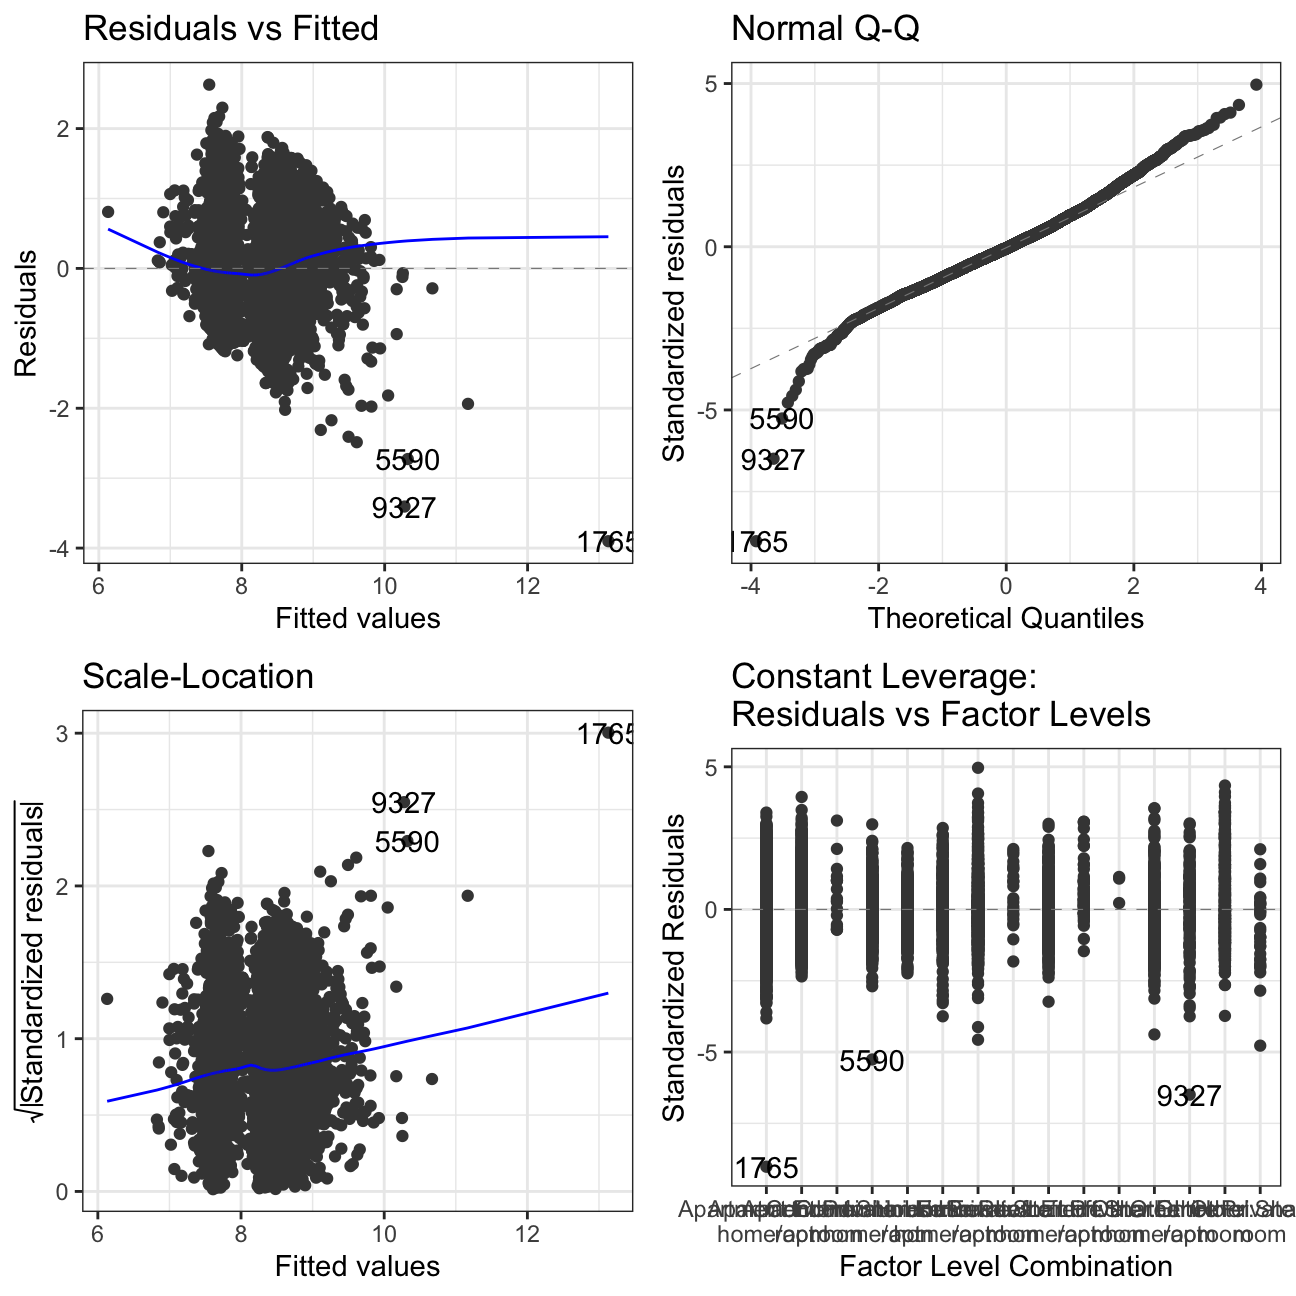
\includegraphics{DataAnalysisvF_files/figure-latex/unnamed-chunk-7-1} \end{center}

\begin{Shaded}
\begin{Highlighting}[]
\KeywordTok{ggsave}\NormalTok{(}\StringTok{"Return Spread Target an Acquirer.png"}\NormalTok{,}
       \DataTypeTok{plot =} \KeywordTok{last\_plot}\NormalTok{(),}
       \DataTypeTok{scale =} \DecValTok{1}\NormalTok{,}
       \DataTypeTok{width =} \DecValTok{20}\NormalTok{,}
       \DataTypeTok{height =} \DecValTok{15}\NormalTok{,}
       \DataTypeTok{units =} \StringTok{"cm"}\NormalTok{,}
       \DataTypeTok{dpi =} \DecValTok{300}\NormalTok{,}
       \DataTypeTok{limitsize =} \OtherTok{TRUE}\NormalTok{)}

\NormalTok{knitr}\OperatorTok{::}\KeywordTok{include\_graphics}\NormalTok{(here}\OperatorTok{::}\KeywordTok{here}\NormalTok{(}\StringTok{"Return Spread Target an Acquirer.png"}\NormalTok{), }\DataTypeTok{error =} \OtherTok{FALSE}\NormalTok{)}
\end{Highlighting}
\end{Shaded}

\begin{center}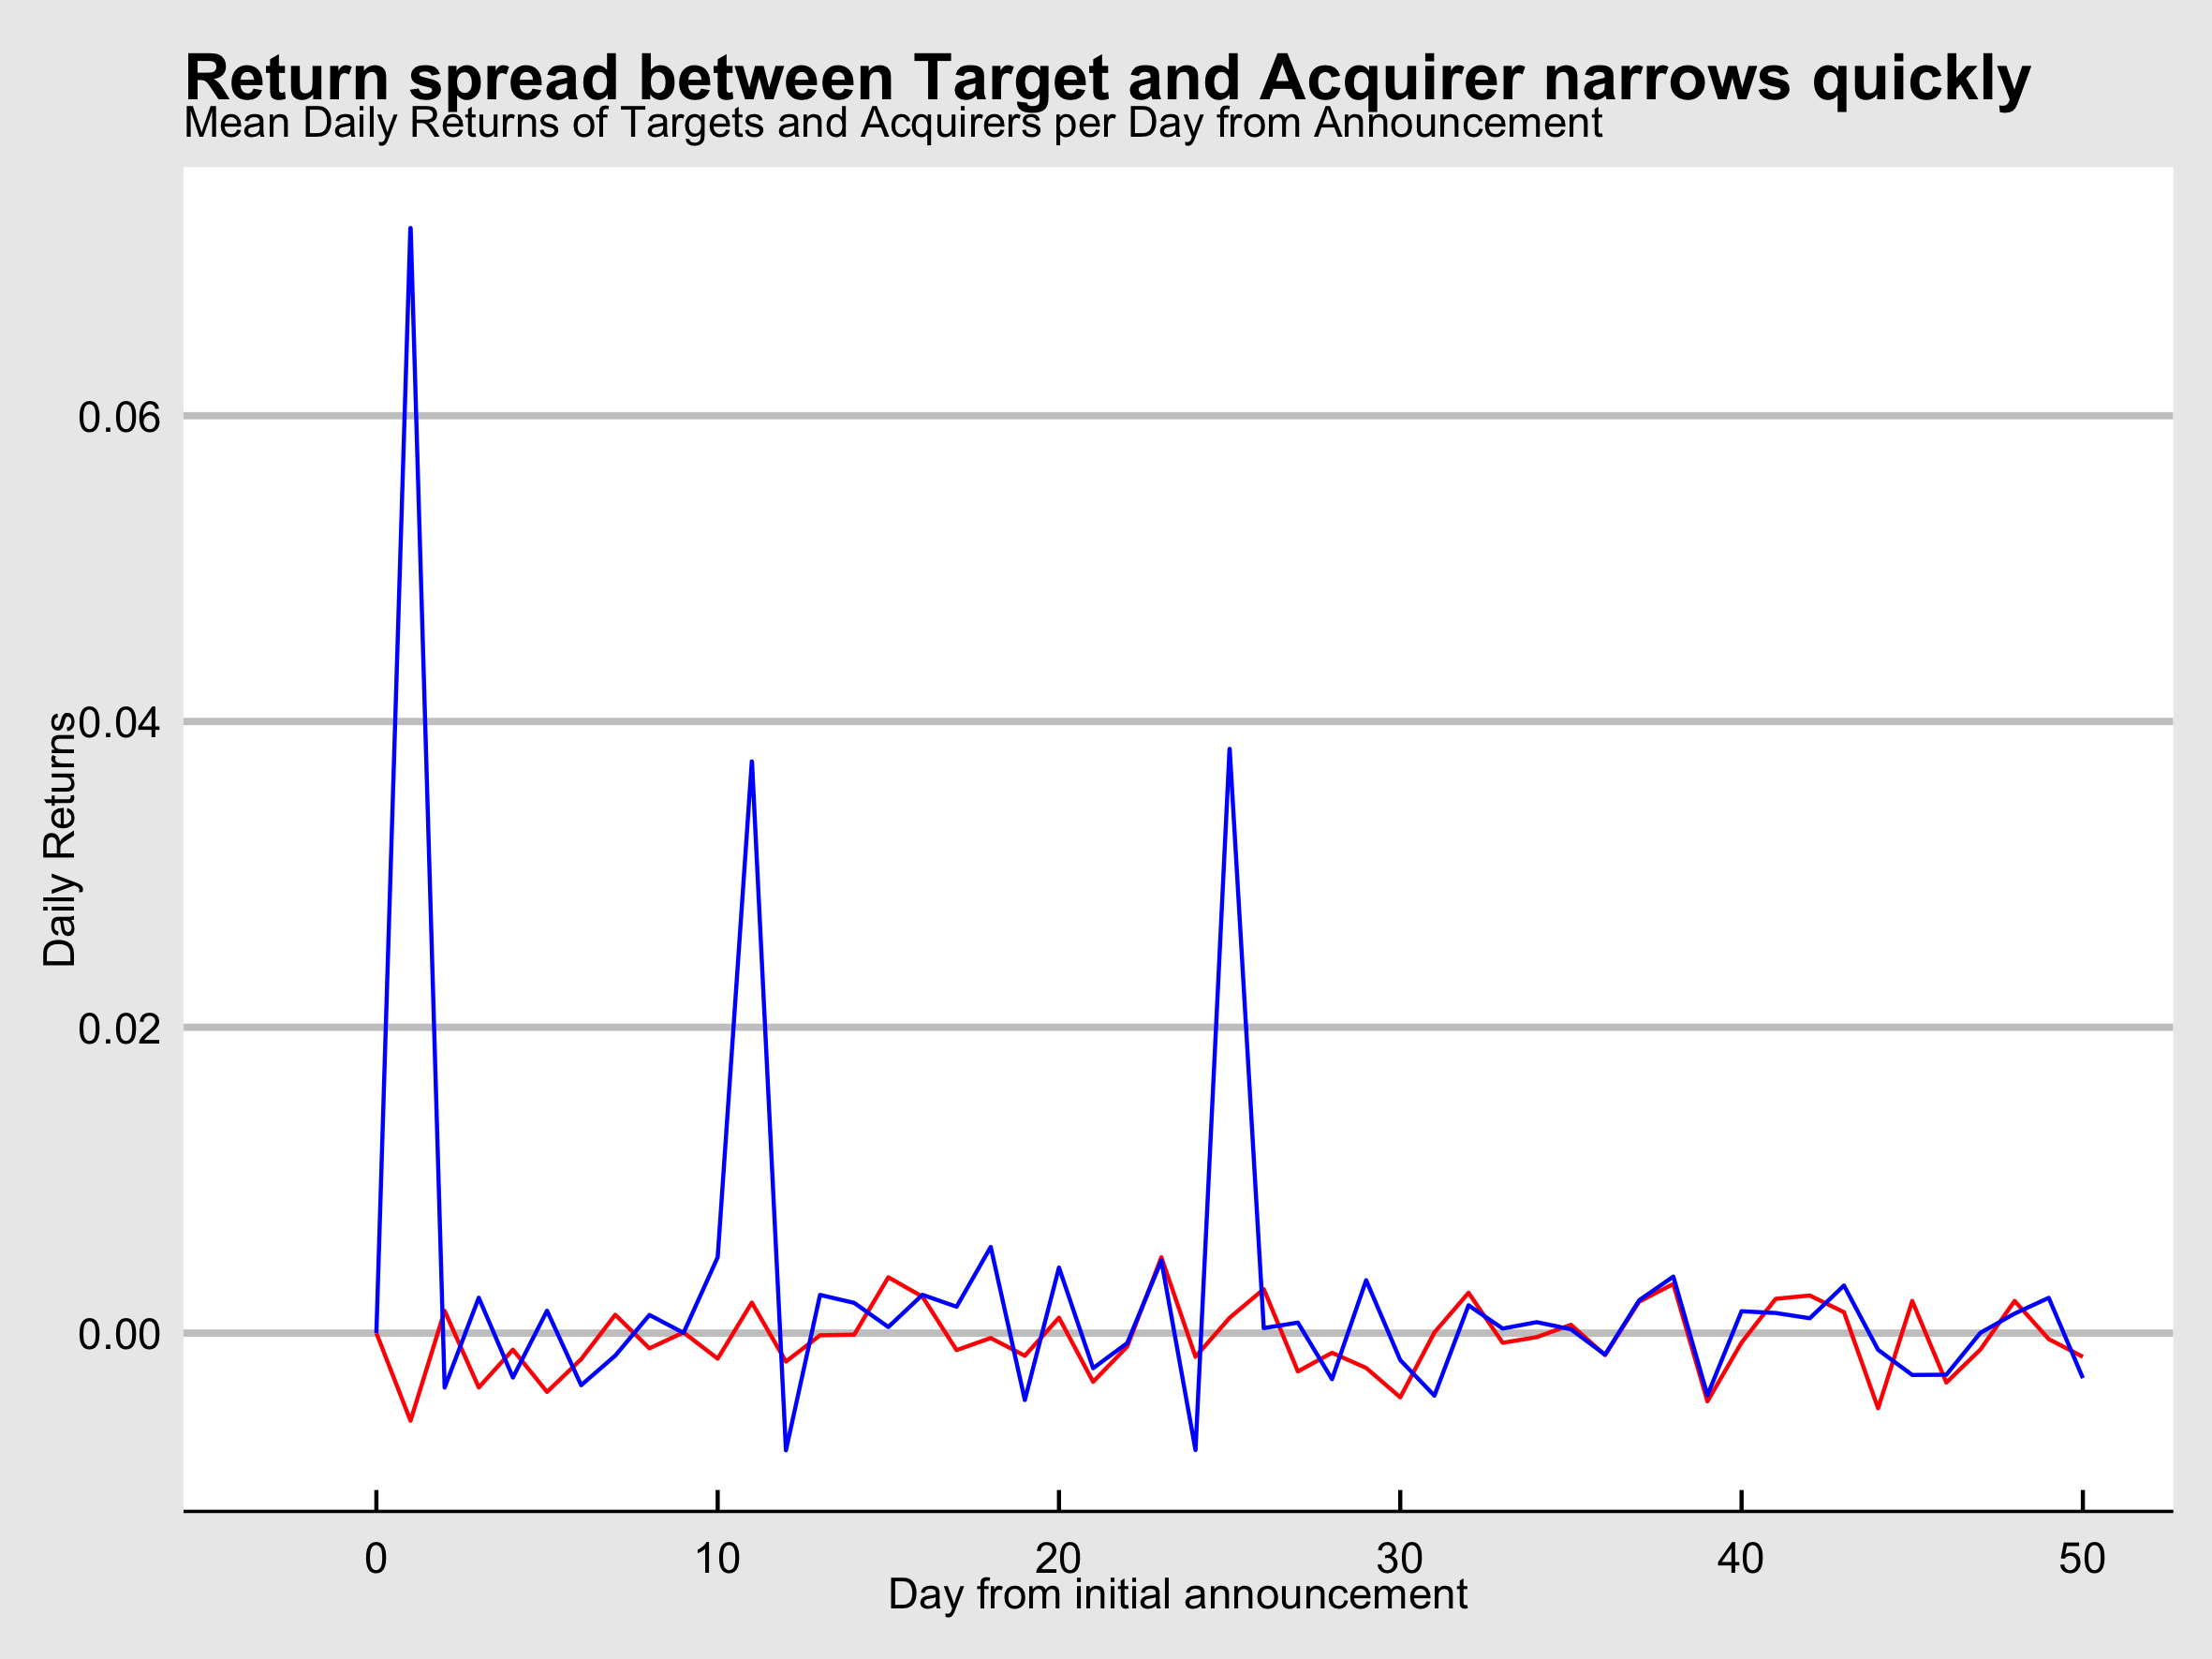
\includegraphics[width=32.81in]{/Users/leifbeckers/Desktop/LBS/Investment Fundamentals/Investment_Fundamentals/Return Spread Target an Acquirer} \end{center}

\begin{Shaded}
\begin{Highlighting}[]
\NormalTok{acq\_tar }\OperatorTok{\%\textgreater{}\%}
\StringTok{  }\KeywordTok{group\_by}\NormalTok{(period) }\OperatorTok{\%\textgreater{}\%}
\StringTok{  }\CommentTok{\# Summarise means per period whilst removing all NAs. Bad data quality forces us to do this}
\StringTok{  }\KeywordTok{summarise}\NormalTok{(}\DataTypeTok{mean\_acq =} \KeywordTok{mean}\NormalTok{(ret\_acq, }\DataTypeTok{na.rm =} \OtherTok{TRUE}\NormalTok{),}
            \DataTypeTok{mean\_tar =} \KeywordTok{mean}\NormalTok{(ret\_tar, }\DataTypeTok{na.rm =} \OtherTok{TRUE}\NormalTok{),}
            \DataTypeTok{mean\_strat =} \KeywordTok{mean}\NormalTok{(ret\_combined, }\DataTypeTok{na.rm =} \OtherTok{TRUE}\NormalTok{)) }\OperatorTok{\%\textgreater{}\%}
\StringTok{  }\KeywordTok{filter}\NormalTok{(period }\OperatorTok{\textless{}=}\StringTok{ }\DecValTok{50}\NormalTok{) }\OperatorTok{\%\textgreater{}\%}
\StringTok{  }\KeywordTok{ggplot}\NormalTok{() }\OperatorTok{+}
\StringTok{  }\KeywordTok{theme\_bw}\NormalTok{() }\OperatorTok{+}
\StringTok{  }\KeywordTok{geom\_line}\NormalTok{(}\KeywordTok{aes}\NormalTok{(}\DataTypeTok{x =}\NormalTok{ period, }\DataTypeTok{y =}\NormalTok{ (mean\_strat)), }\DataTypeTok{colour =} \StringTok{"green"}\NormalTok{) }\OperatorTok{+}\StringTok{ }\CommentTok{\# Portfolio }
\StringTok{  }\KeywordTok{labs}\NormalTok{(}\DataTypeTok{title =} \StringTok{"Target and Acquirer Spread drives Strategy Return"}\NormalTok{,}
       \DataTypeTok{subtitle =} \StringTok{"Mean Daily Returns of Strategy per Day from Announcement"}\NormalTok{,}
       \DataTypeTok{y =} \StringTok{"Daily Returns"}\NormalTok{,}
       \DataTypeTok{x =} \StringTok{"Day from initial announcement"}\NormalTok{) }\OperatorTok{+}\StringTok{ }
\StringTok{  }\KeywordTok{theme\_economist\_white}\NormalTok{()}
\end{Highlighting}
\end{Shaded}

\begin{center}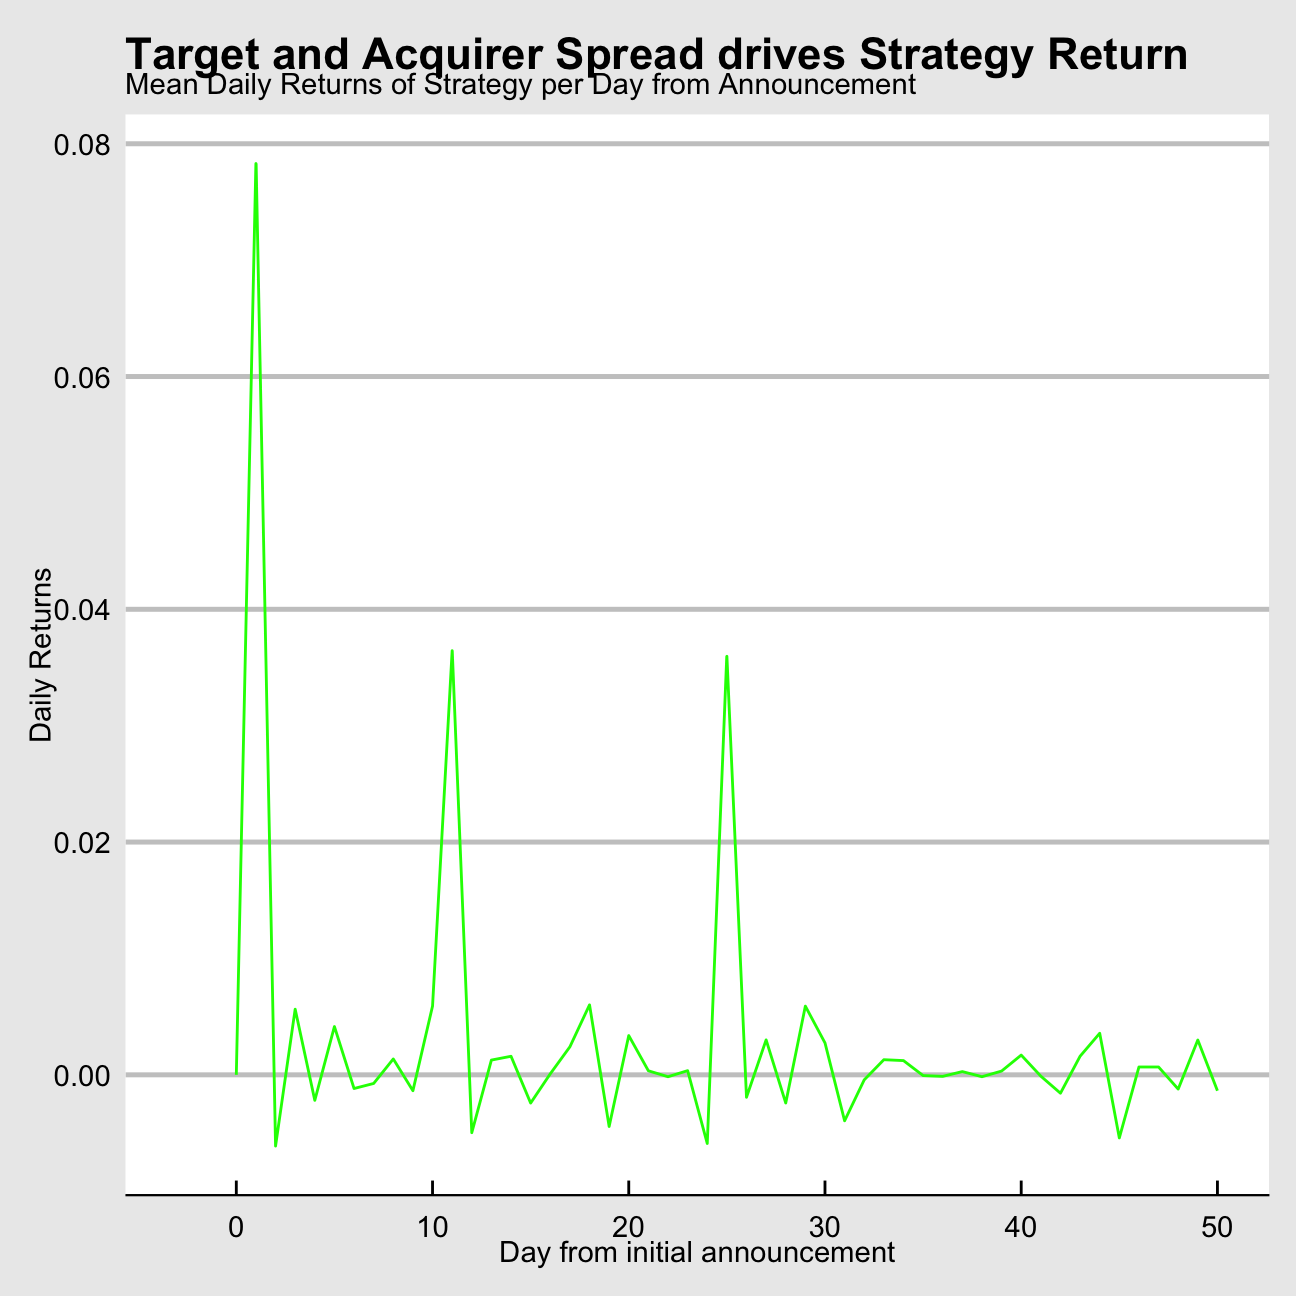
\includegraphics{DataAnalysisvF_files/figure-latex/unnamed-chunk-7-3} \end{center}

\begin{Shaded}
\begin{Highlighting}[]
\KeywordTok{ggsave}\NormalTok{(}\StringTok{"Strategy Return from Spread.png"}\NormalTok{,}
       \DataTypeTok{plot =} \KeywordTok{last\_plot}\NormalTok{(),}
       \DataTypeTok{scale =} \DecValTok{1}\NormalTok{,}
       \DataTypeTok{width =} \DecValTok{20}\NormalTok{,}
       \DataTypeTok{height =} \DecValTok{15}\NormalTok{,}
       \DataTypeTok{units =} \StringTok{"cm"}\NormalTok{,}
       \DataTypeTok{dpi =} \DecValTok{300}\NormalTok{,}
       \DataTypeTok{limitsize =} \OtherTok{TRUE}\NormalTok{)}

\NormalTok{knitr}\OperatorTok{::}\KeywordTok{include\_graphics}\NormalTok{(here}\OperatorTok{::}\KeywordTok{here}\NormalTok{(}\StringTok{"Strategy Return from Spread.png"}\NormalTok{), }\DataTypeTok{error =} \OtherTok{FALSE}\NormalTok{)}
\end{Highlighting}
\end{Shaded}

\begin{center}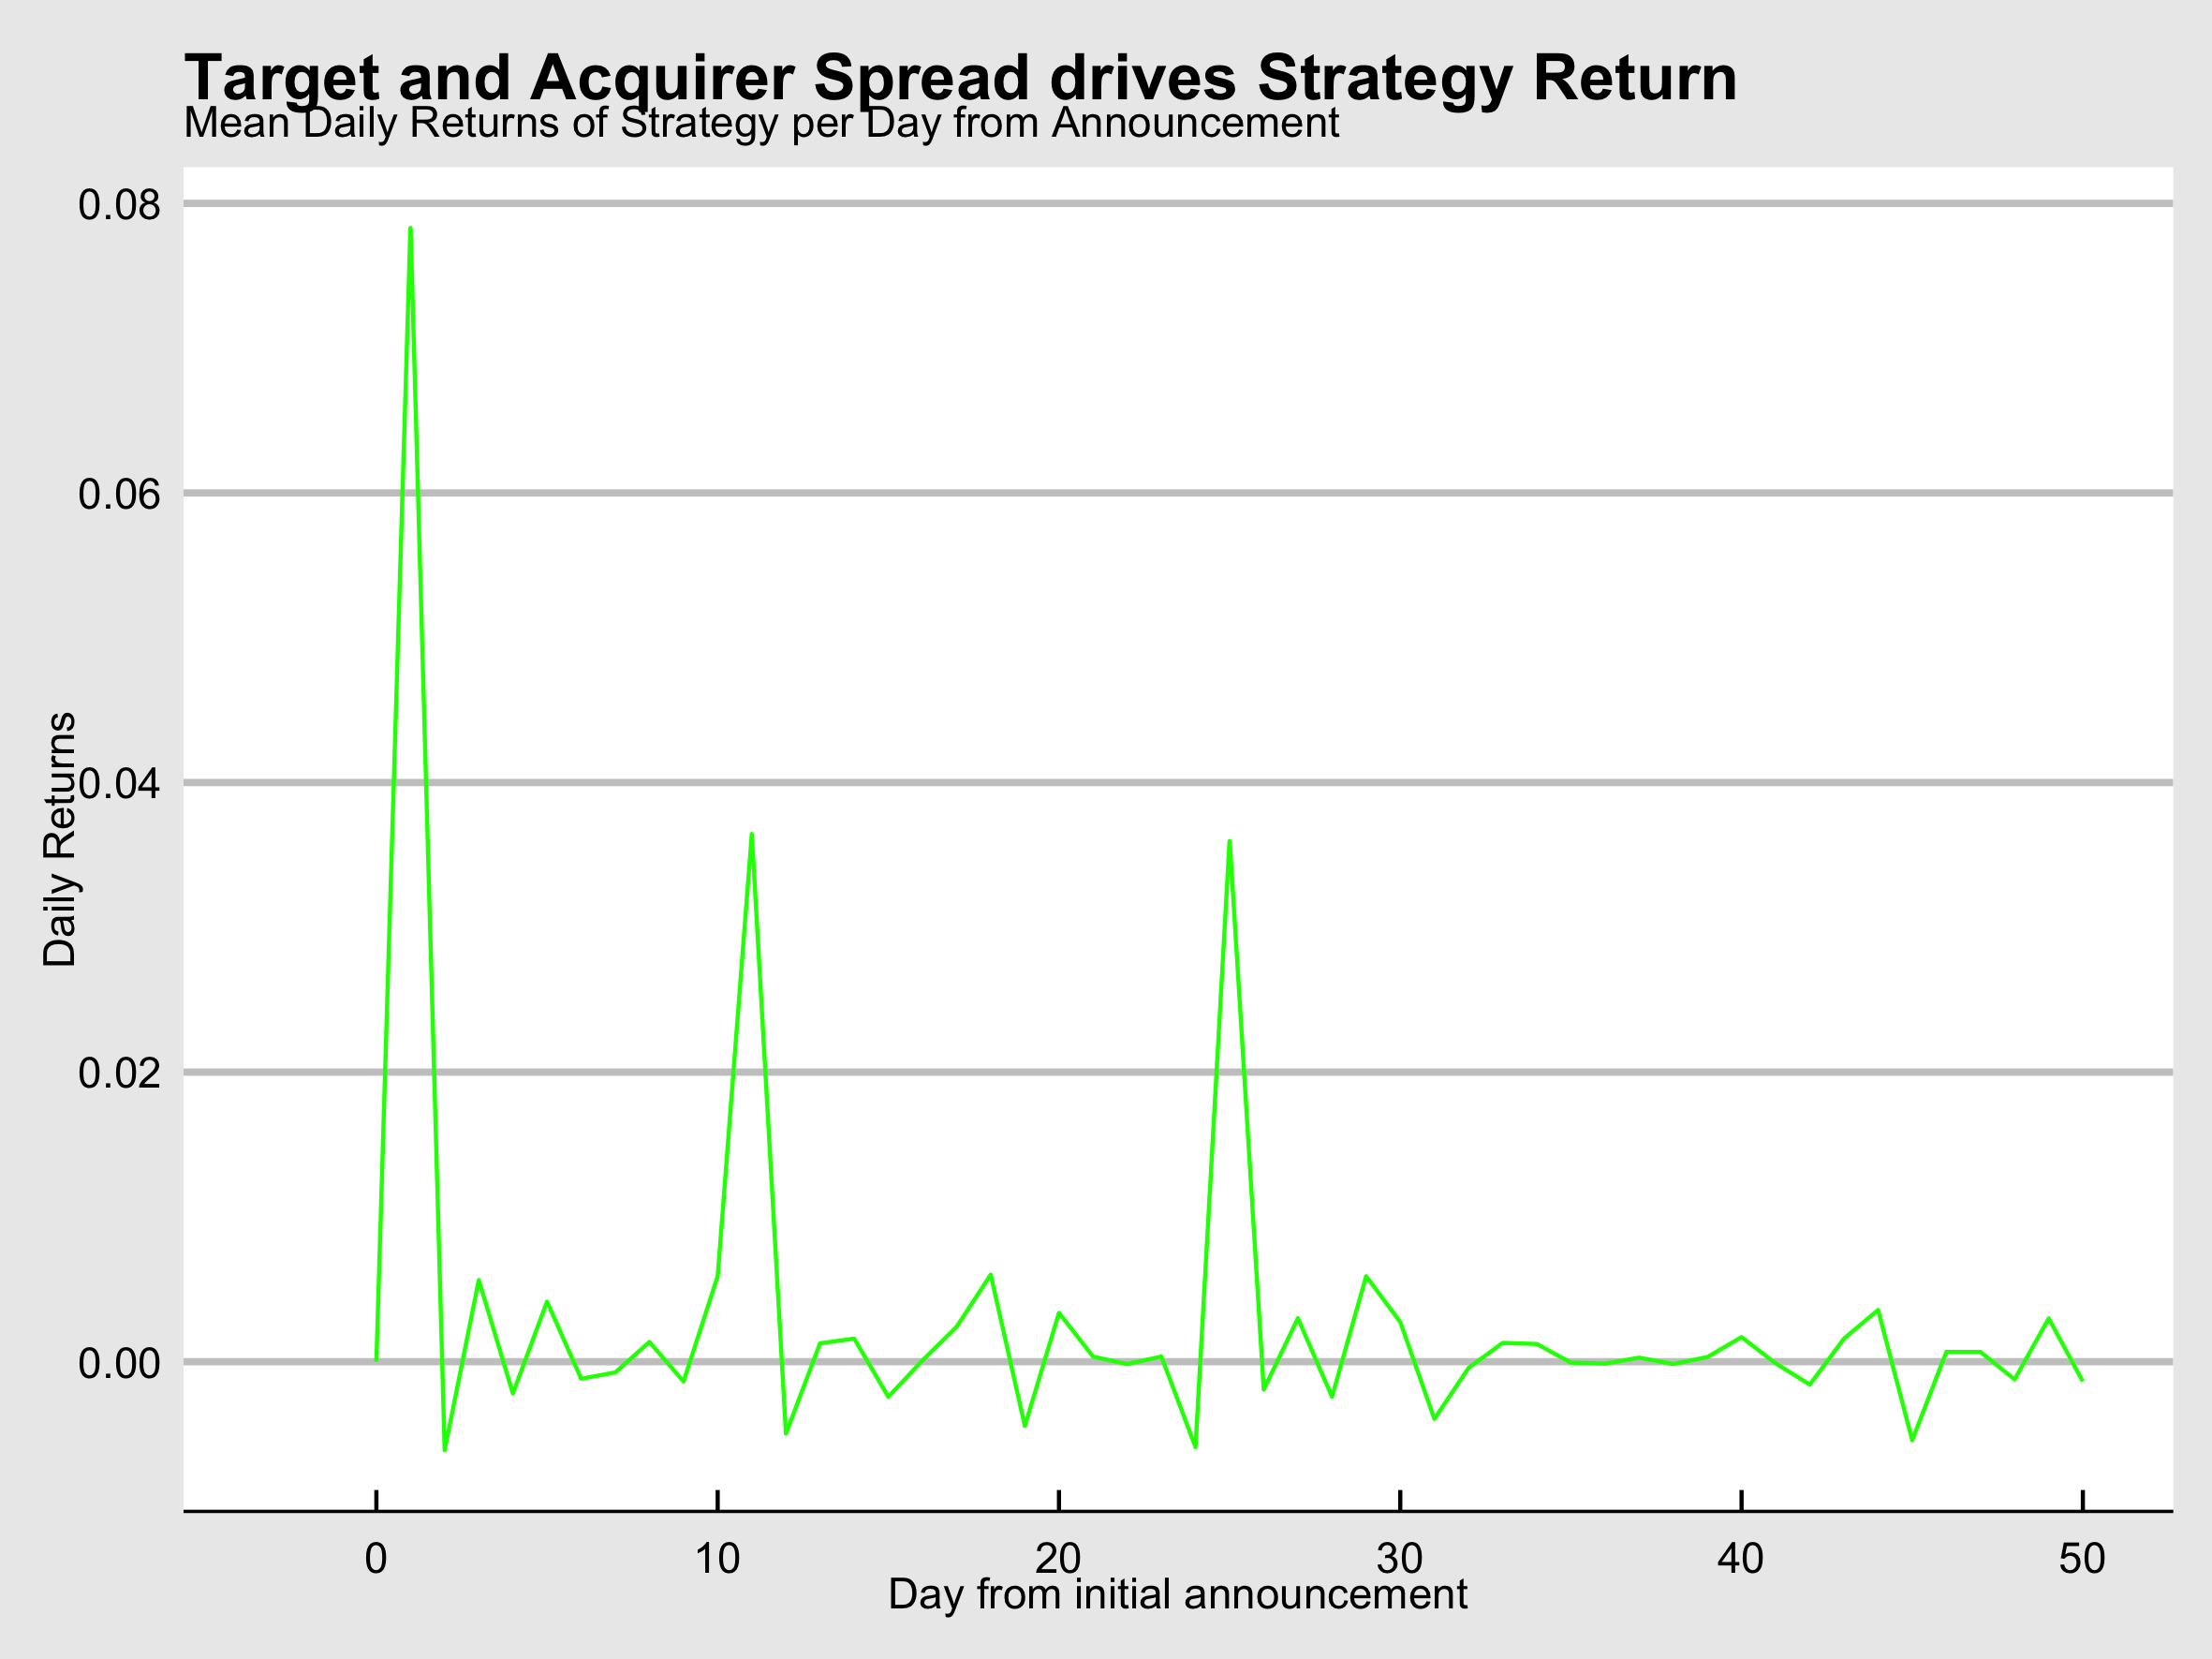
\includegraphics[width=32.81in]{/Users/leifbeckers/Desktop/LBS/Investment Fundamentals/Investment_Fundamentals/Strategy Return from Spread} \end{center}

\hypertarget{cumulative-return}{%
\subsection{Cumulative Return}\label{cumulative-return}}

\hypertarget{acquirer}{%
\subsubsection{Acquirer}\label{acquirer}}

\begin{Shaded}
\begin{Highlighting}[]
\CommentTok{\# Cumulative return for acquirer}
\NormalTok{initial\_acq \textless{}{-}}\StringTok{ }\NormalTok{acq\_tar }\OperatorTok{\%\textgreater{}\%}
\StringTok{  }\KeywordTok{filter}\NormalTok{(period }\OperatorTok{==}\StringTok{ }\DecValTok{0}\NormalTok{) }\OperatorTok{\%\textgreater{}\%}
\StringTok{  }\KeywordTok{rename}\NormalTok{(}\DataTypeTok{initial\_acq =}\NormalTok{ close\_acquirer) }\OperatorTok{\%\textgreater{}\%}
\StringTok{  }\KeywordTok{select}\NormalTok{(acquirer, target, initial\_acq) }\OperatorTok{\%\textgreater{}\%}
\StringTok{  }\KeywordTok{distinct}\NormalTok{()}

\NormalTok{cum\_acq \textless{}{-}}\StringTok{ }\KeywordTok{left\_join}\NormalTok{(acq\_tar, initial\_acq, }\DataTypeTok{by =} \KeywordTok{c}\NormalTok{(}\StringTok{"acquirer"}\NormalTok{, }\StringTok{"target"}\NormalTok{)) }\OperatorTok{\%\textgreater{}\%}
\StringTok{  }\KeywordTok{mutate}\NormalTok{(}\DataTypeTok{cum\_ret\_acq =} \KeywordTok{ifelse}\NormalTok{(period }\OperatorTok{\textgreater{}}\StringTok{ }\DecValTok{{-}1}\NormalTok{, close\_acquirer}\OperatorTok{/}\NormalTok{initial\_acq }\OperatorTok{{-}}\StringTok{ }\DecValTok{1}\NormalTok{, }\OtherTok{NA}\NormalTok{)) }\OperatorTok{\%\textgreater{}\%}
\StringTok{  }\KeywordTok{group\_by}\NormalTok{(period) }\OperatorTok{\%\textgreater{}\%}
\StringTok{  }\KeywordTok{summarise}\NormalTok{(}\DataTypeTok{mean\_cum\_ret\_acq =} \KeywordTok{mean}\NormalTok{(cum\_ret\_acq, }\DataTypeTok{na.rm =}\OtherTok{TRUE}\NormalTok{)) }\OperatorTok{\%\textgreater{}\%}
\StringTok{  }\KeywordTok{filter}\NormalTok{(period }\OperatorTok{\textless{}=}\StringTok{ }\DecValTok{50}\NormalTok{)}
\end{Highlighting}
\end{Shaded}

\hypertarget{target}{%
\subsubsection{Target}\label{target}}

\begin{Shaded}
\begin{Highlighting}[]
\CommentTok{\# Cumulative return for target}
\NormalTok{initial\_tar \textless{}{-}}\StringTok{ }\NormalTok{acq\_tar }\OperatorTok{\%\textgreater{}\%}
\StringTok{  }\KeywordTok{filter}\NormalTok{(period }\OperatorTok{==}\StringTok{ }\DecValTok{0}\NormalTok{) }\OperatorTok{\%\textgreater{}\%}
\StringTok{  }\KeywordTok{rename}\NormalTok{(}\DataTypeTok{initial\_tar =}\NormalTok{ close\_target) }\OperatorTok{\%\textgreater{}\%}
\StringTok{  }\KeywordTok{select}\NormalTok{(acquirer, target, initial\_tar) }\OperatorTok{\%\textgreater{}\%}\StringTok{ }
\StringTok{  }\KeywordTok{distinct}\NormalTok{()}

\NormalTok{cum\_tar \textless{}{-}}\StringTok{ }\KeywordTok{left\_join}\NormalTok{(acq\_tar, initial\_tar, }\DataTypeTok{by =} \KeywordTok{c}\NormalTok{(}\StringTok{"acquirer"}\NormalTok{, }\StringTok{"target"}\NormalTok{)) }\OperatorTok{\%\textgreater{}\%}
\StringTok{  }\KeywordTok{mutate}\NormalTok{(}\DataTypeTok{cum\_ret\_tar =} \KeywordTok{ifelse}\NormalTok{(period }\OperatorTok{\textgreater{}}\StringTok{ }\DecValTok{{-}1}\NormalTok{, close\_target}\OperatorTok{/}\NormalTok{initial\_tar }\OperatorTok{{-}}\StringTok{ }\DecValTok{1}\NormalTok{, }\OtherTok{NA}\NormalTok{)) }\OperatorTok{\%\textgreater{}\%}
\StringTok{  }\KeywordTok{group\_by}\NormalTok{(period) }\OperatorTok{\%\textgreater{}\%}
\StringTok{  }\KeywordTok{summarise}\NormalTok{(}\DataTypeTok{mean\_cum\_ret\_tar =} \KeywordTok{mean}\NormalTok{(cum\_ret\_tar, }\DataTypeTok{na.rm =}\OtherTok{TRUE}\NormalTok{)) }\OperatorTok{\%\textgreater{}\%}
\StringTok{  }\KeywordTok{filter}\NormalTok{(period }\OperatorTok{\textless{}=}\StringTok{ }\DecValTok{50}\NormalTok{)}
\end{Highlighting}
\end{Shaded}

\hypertarget{cumulative-return-spread}{%
\subsubsection{Cumulative Return
Spread}\label{cumulative-return-spread}}

\begin{Shaded}
\begin{Highlighting}[]
\CommentTok{\# Combine all}
\NormalTok{cum\_all \textless{}{-}}\StringTok{ }\KeywordTok{left\_join}\NormalTok{(cum\_acq, cum\_tar, }\DataTypeTok{by =} \StringTok{"period"}\NormalTok{) }\OperatorTok{\%\textgreater{}\%}
\StringTok{  }\KeywordTok{filter}\NormalTok{(period }\OperatorTok{\textless{}=}\StringTok{ }\DecValTok{50}\NormalTok{)}
  

\KeywordTok{ggplot}\NormalTok{(cum\_all) }\OperatorTok{+}
\StringTok{  }
\StringTok{  }\KeywordTok{geom\_line}\NormalTok{(}\KeywordTok{aes}\NormalTok{(}\DataTypeTok{x =}\NormalTok{ period, }\DataTypeTok{y =}\NormalTok{ mean\_cum\_ret\_tar), }\DataTypeTok{colour =} \StringTok{"blue"}\NormalTok{) }\OperatorTok{+}
\StringTok{  }\KeywordTok{geom\_line}\NormalTok{(}\KeywordTok{aes}\NormalTok{(}\DataTypeTok{x =}\NormalTok{ period, }\DataTypeTok{y =}\NormalTok{ mean\_cum\_ret\_acq), }\DataTypeTok{colour =} \StringTok{"red"}\NormalTok{) }\OperatorTok{+}
\StringTok{  }\KeywordTok{theme\_bw}\NormalTok{() }\OperatorTok{+}
\StringTok{  }\KeywordTok{labs}\NormalTok{(}\DataTypeTok{subtitle =} \StringTok{"Mean Cumulative Return {-} Investments start 1 day after announcement"}\NormalTok{,}
       \DataTypeTok{title =} \StringTok{"Target outperformance in cumulative return driven by early gains"}\NormalTok{,}
       \DataTypeTok{y =} \StringTok{"Cumulative Return"}\NormalTok{,}
       \DataTypeTok{x =} \StringTok{"Day from announcement"}\NormalTok{) }\OperatorTok{+}\StringTok{ }
\StringTok{  }\KeywordTok{theme\_economist\_white}\NormalTok{()}
\end{Highlighting}
\end{Shaded}

\begin{center}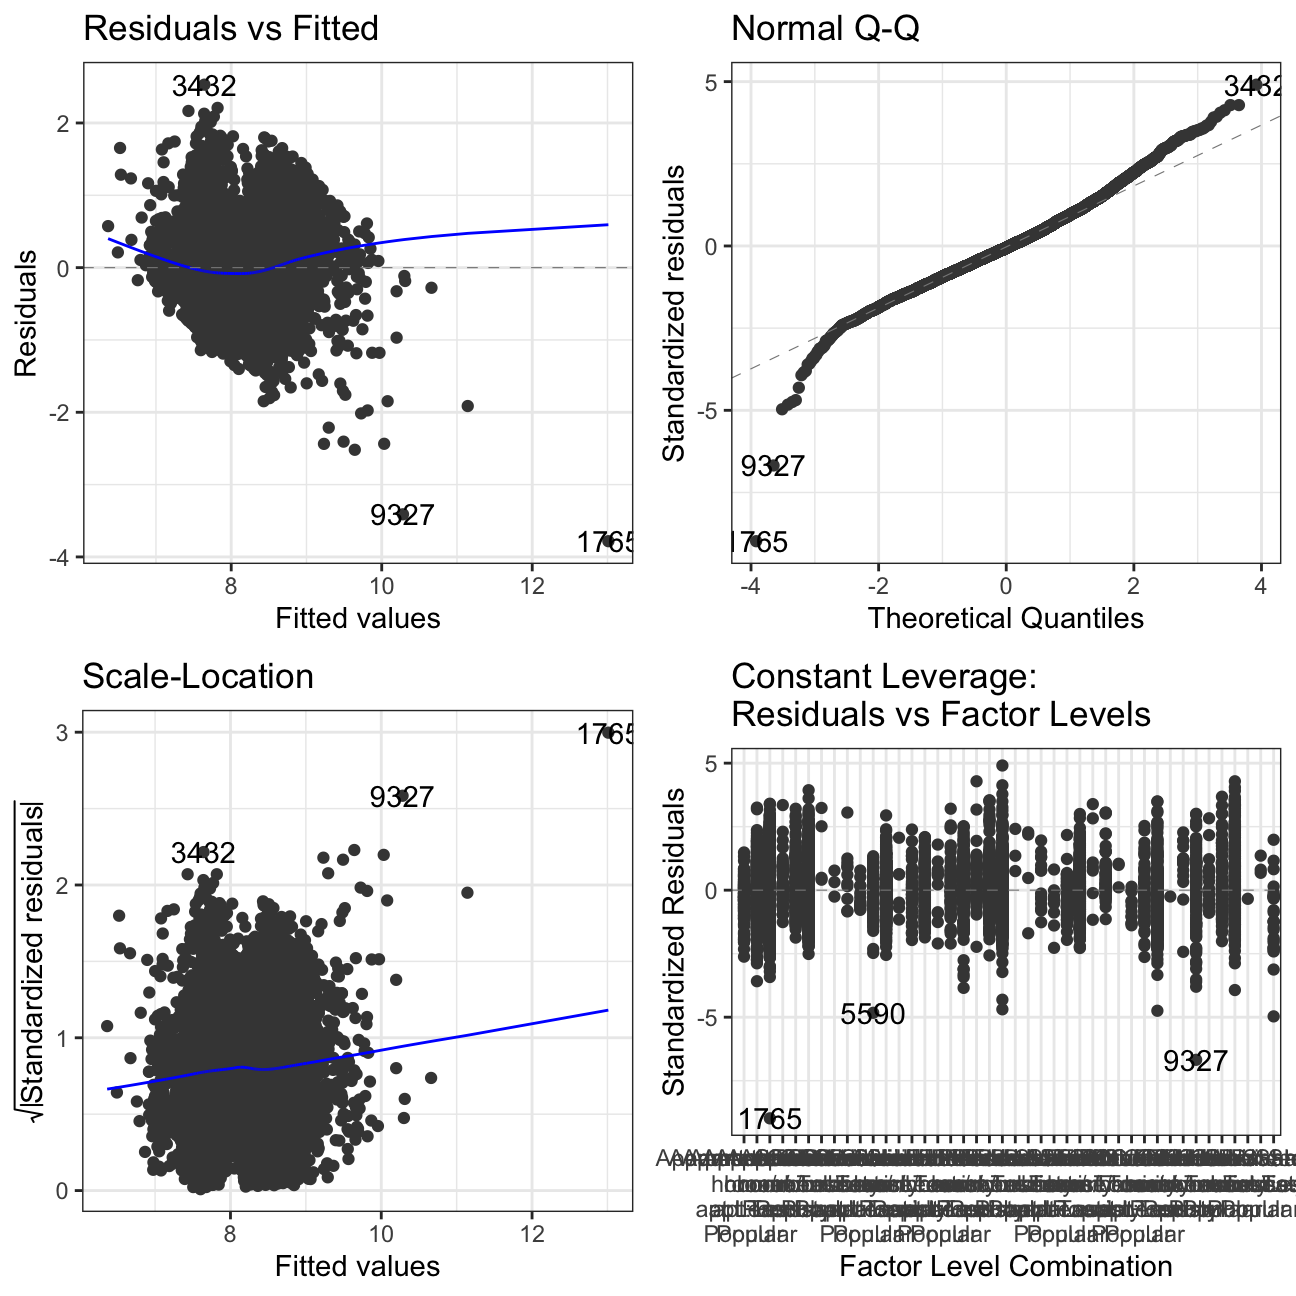
\includegraphics{DataAnalysisvF_files/figure-latex/unnamed-chunk-10-1} \end{center}

\begin{Shaded}
\begin{Highlighting}[]
\KeywordTok{ggsave}\NormalTok{(}\StringTok{"Cumulative Returns Target and Acquirer.png"}\NormalTok{,}
       \DataTypeTok{plot =} \KeywordTok{last\_plot}\NormalTok{(),}
       \DataTypeTok{scale =} \DecValTok{1}\NormalTok{,}
       \DataTypeTok{width =} \DecValTok{20}\NormalTok{,}
       \DataTypeTok{height =} \DecValTok{15}\NormalTok{,}
       \DataTypeTok{units =} \StringTok{"cm"}\NormalTok{,}
       \DataTypeTok{dpi =} \DecValTok{300}\NormalTok{,}
       \DataTypeTok{limitsize =} \OtherTok{TRUE}\NormalTok{)}

\NormalTok{knitr}\OperatorTok{::}\KeywordTok{include\_graphics}\NormalTok{(here}\OperatorTok{::}\KeywordTok{here}\NormalTok{(}\StringTok{"Cumulative Returns Target and Acquirer.png"}\NormalTok{), }\DataTypeTok{error =} \OtherTok{FALSE}\NormalTok{)}
\end{Highlighting}
\end{Shaded}

\begin{center}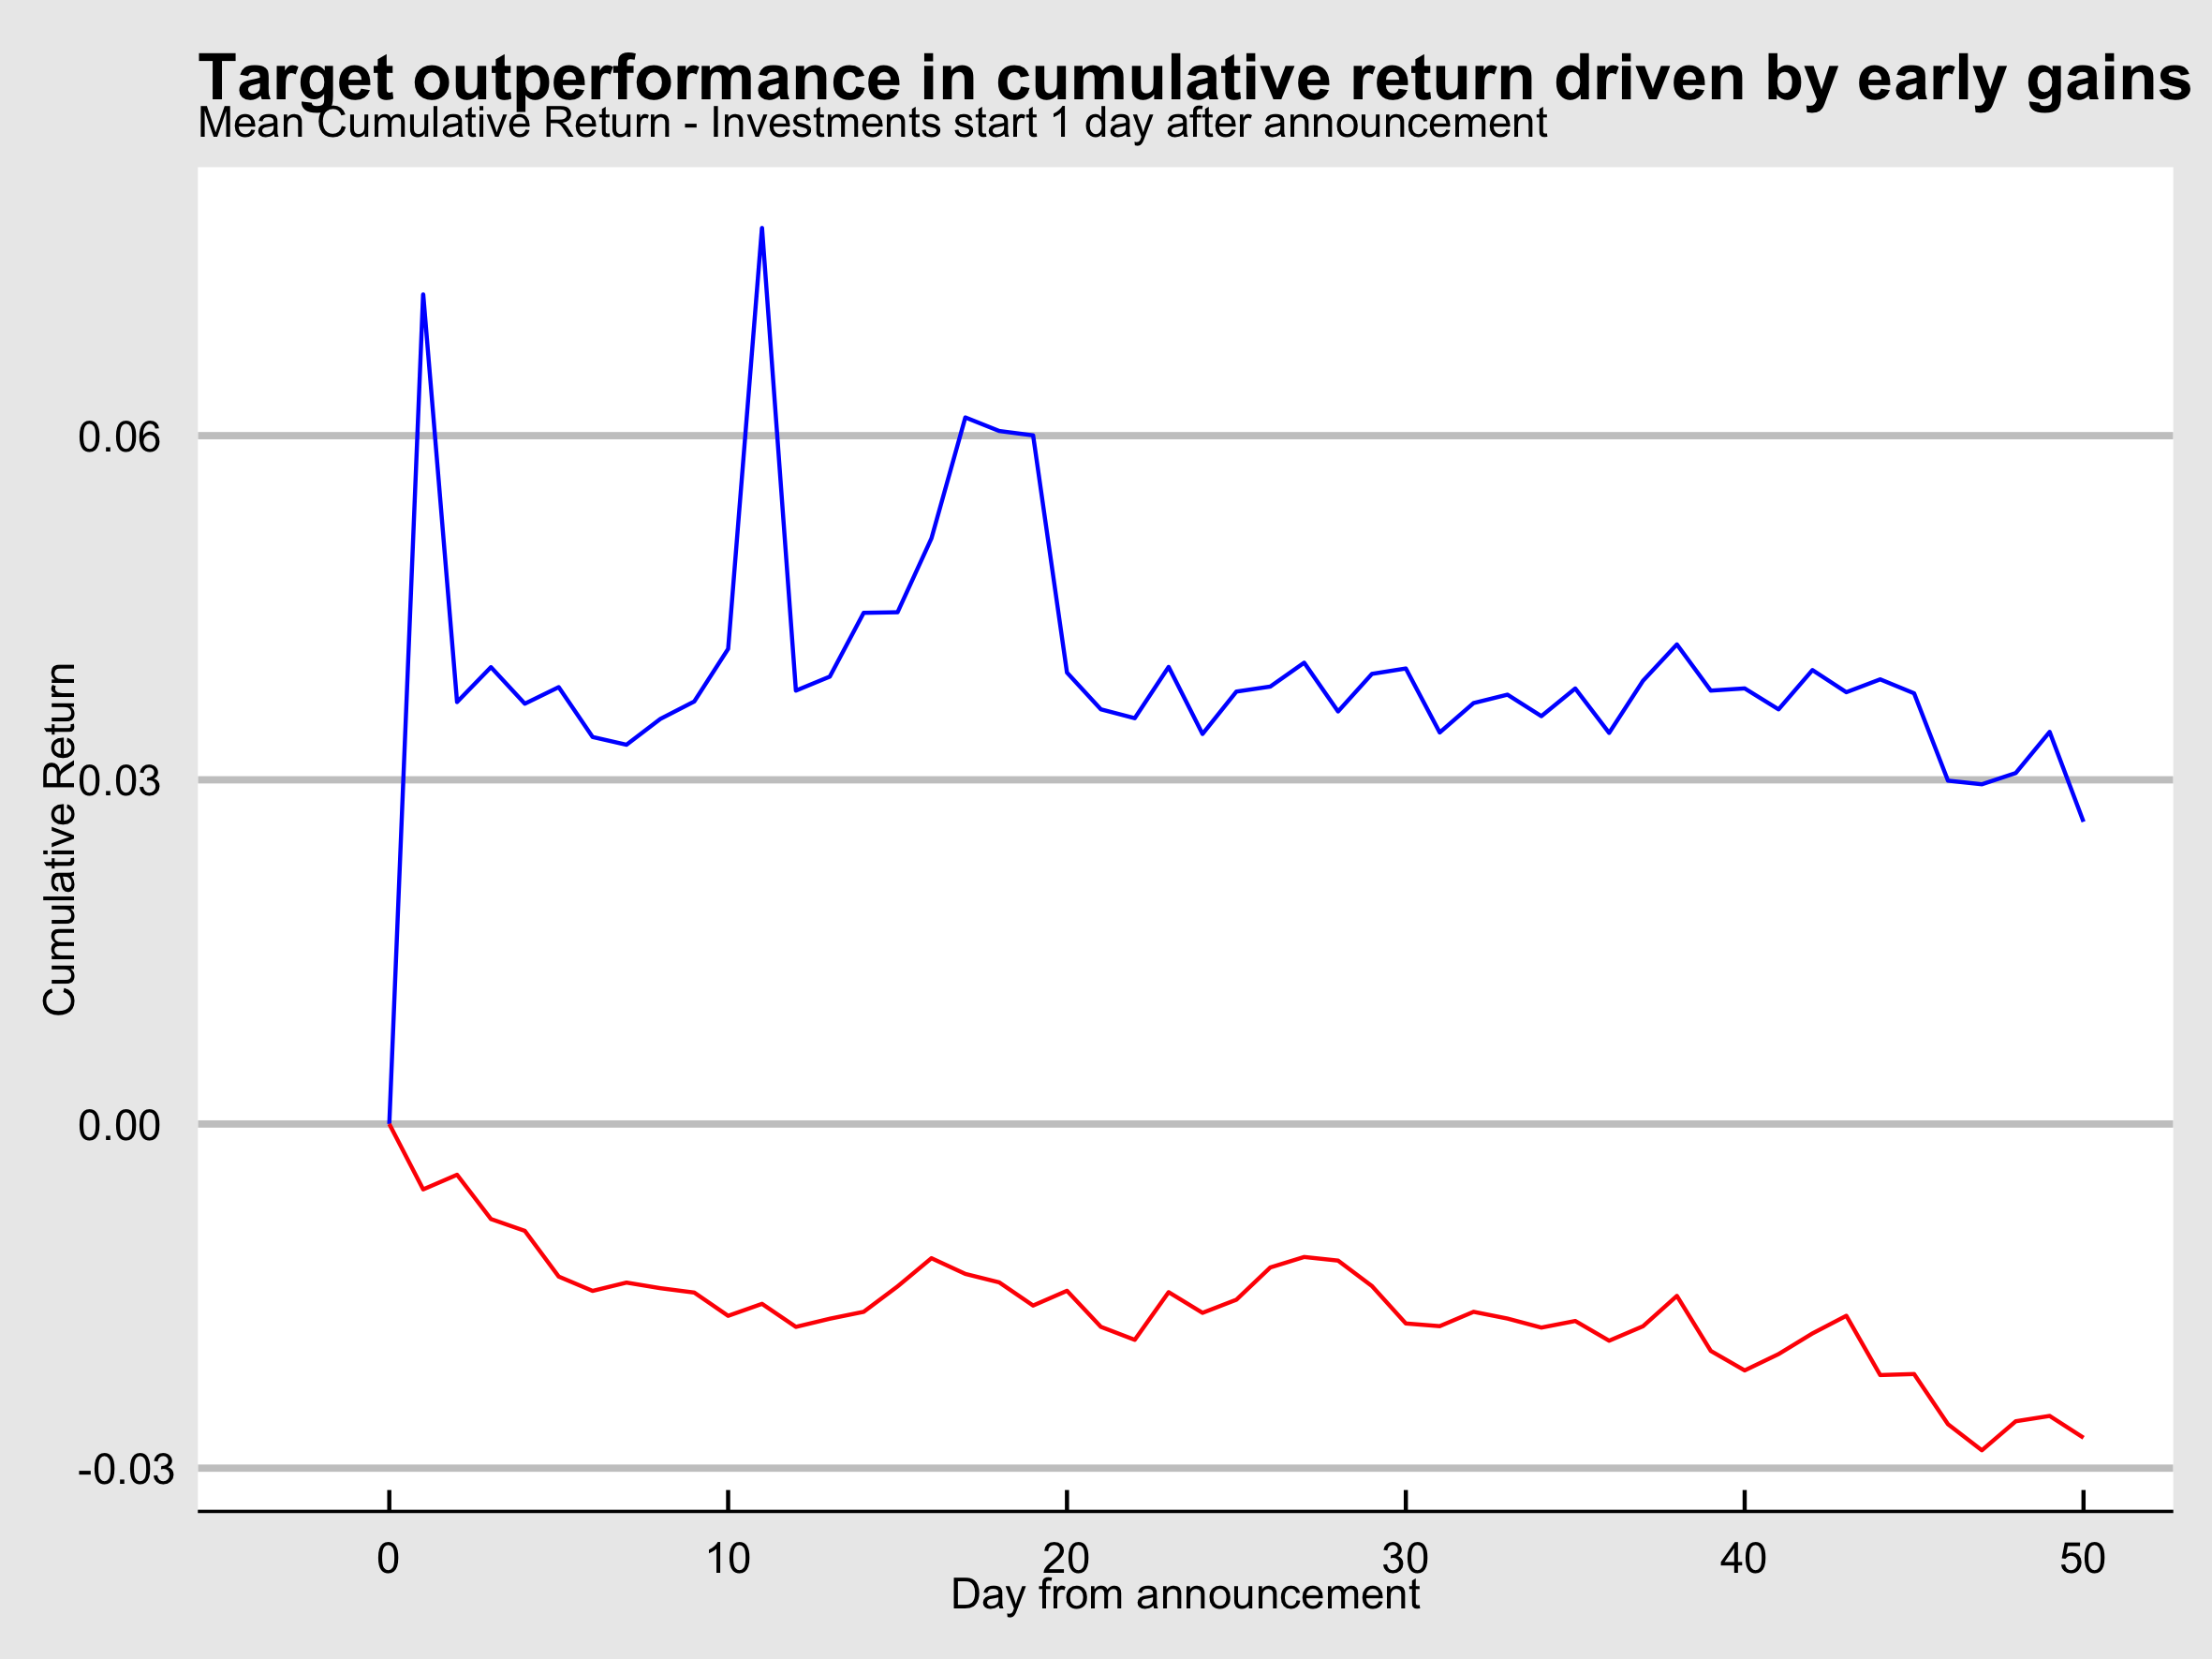
\includegraphics[width=32.81in]{/Users/leifbeckers/Desktop/LBS/Investment Fundamentals/Investment_Fundamentals/Cumulative Returns Target and Acquirer} \end{center}

\hypertarget{correlation-between-return-and-deal-completion}{%
\subsection{Correlation between return and deal
completion}\label{correlation-between-return-and-deal-completion}}

\hypertarget{acquirer-1}{%
\subsubsection{Acquirer}\label{acquirer-1}}

\begin{Shaded}
\begin{Highlighting}[]
\NormalTok{end\_acq \textless{}{-}}\StringTok{ }\NormalTok{acq\_tar }\OperatorTok{\%\textgreater{}\%}
\StringTok{  }\KeywordTok{mutate}\NormalTok{(}\DataTypeTok{diff =}\NormalTok{ close\_date }\OperatorTok{{-}}\StringTok{ }\NormalTok{date) }\OperatorTok{\%\textgreater{}\%}
\StringTok{  }\KeywordTok{filter}\NormalTok{(diff }\OperatorTok{==}\StringTok{ }\DecValTok{0}\NormalTok{) }\OperatorTok{\%\textgreater{}\%}
\StringTok{  }\KeywordTok{rename}\NormalTok{(}\DataTypeTok{end\_acq =}\NormalTok{ close\_acquirer) }\OperatorTok{\%\textgreater{}\%}
\StringTok{  }\KeywordTok{select}\NormalTok{(acquirer, period, target, end\_acq, DealStatus) }\OperatorTok{\%\textgreater{}\%}
\StringTok{  }\KeywordTok{distinct}\NormalTok{()}


\NormalTok{deal\_ret\_acq \textless{}{-}}\StringTok{ }\KeywordTok{left\_join}\NormalTok{(end\_acq, initial\_acq, }\DataTypeTok{by =} \KeywordTok{c}\NormalTok{(}\StringTok{"acquirer"}\NormalTok{, }\StringTok{"target"}\NormalTok{)) }\OperatorTok{\%\textgreater{}\%}\StringTok{ }
\StringTok{  }\KeywordTok{distinct}\NormalTok{() }\OperatorTok{\%\textgreater{}\%}
\StringTok{  }\KeywordTok{mutate}\NormalTok{(}\DataTypeTok{annualised\_ret =}\NormalTok{ (end\_acq}\OperatorTok{/}\NormalTok{initial\_acq)}\OperatorTok{\^{}}\NormalTok{(}\DecValTok{252}\OperatorTok{/}\NormalTok{period) }\OperatorTok{{-}}\StringTok{ }\DecValTok{1}\NormalTok{) }\OperatorTok{\%\textgreater{}\%}
\StringTok{  }\KeywordTok{group\_by}\NormalTok{(DealStatus) }\OperatorTok{\%\textgreater{}\%}
\StringTok{  }\KeywordTok{summarise}\NormalTok{(}\DataTypeTok{mean\_annualised\_acq\_ret =} \KeywordTok{median}\NormalTok{(annualised\_ret, }\DataTypeTok{na.rm =} \OtherTok{TRUE}\NormalTok{))}

\NormalTok{deal\_ret\_acq}
\end{Highlighting}
\end{Shaded}

 
  \providecommand{\huxb}[2]{\arrayrulecolor[RGB]{#1}\global\arrayrulewidth=#2pt}
  \providecommand{\huxvb}[2]{\color[RGB]{#1}\vrule width #2pt}
  \providecommand{\huxtpad}[1]{\rule{0pt}{#1}}
  \providecommand{\huxbpad}[1]{\rule[-#1]{0pt}{#1}}

\begin{table}[ht]
\begin{centerbox}
\begin{threeparttable}
 \label{tab:unnamed-chunk-11}
\setlength{\tabcolsep}{0pt}
\begin{tabular}{l l}


\hhline{>{\huxb{0, 0, 0}{0.4}}->{\huxb{0, 0, 0}{0.4}}-}
\arrayrulecolor{black}

\multicolumn{1}{!{\huxvb{0, 0, 0}{0.4}}l!{\huxvb{0, 0, 0}{0}}}{\huxtpad{6pt + 1em}\raggedright \hspace{6pt} \textbf{DealStatus} \hspace{6pt}\huxbpad{6pt}} &
\multicolumn{1}{r!{\huxvb{0, 0, 0}{0.4}}}{\huxtpad{6pt + 1em}\raggedleft \hspace{6pt} \textbf{mean\_annualised\_acq\_ret} \hspace{6pt}\huxbpad{6pt}} \tabularnewline[-0.5pt]


\hhline{>{\huxb{0, 0, 0}{0.4}}->{\huxb{0, 0, 0}{0.4}}-}
\arrayrulecolor{black}

\multicolumn{1}{!{\huxvb{0, 0, 0}{0.4}}l!{\huxvb{0, 0, 0}{0}}}{\cellcolor[RGB]{242, 242, 242}\huxtpad{6pt + 1em}\raggedright \hspace{6pt} Completed \hspace{6pt}\huxbpad{6pt}} &
\multicolumn{1}{r!{\huxvb{0, 0, 0}{0.4}}}{\cellcolor[RGB]{242, 242, 242}\huxtpad{6pt + 1em}\raggedleft \hspace{6pt} -0.0129 \hspace{6pt}\huxbpad{6pt}} \tabularnewline[-0.5pt]


\hhline{>{\huxb{0, 0, 0}{0.4}}|>{\huxb{0, 0, 0}{0.4}}|}
\arrayrulecolor{black}

\multicolumn{1}{!{\huxvb{0, 0, 0}{0.4}}l!{\huxvb{0, 0, 0}{0}}}{\huxtpad{6pt + 1em}\raggedright \hspace{6pt} Failed \hspace{6pt}\huxbpad{6pt}} &
\multicolumn{1}{r!{\huxvb{0, 0, 0}{0.4}}}{\huxtpad{6pt + 1em}\raggedleft \hspace{6pt} -0.46~~ \hspace{6pt}\huxbpad{6pt}} \tabularnewline[-0.5pt]


\hhline{>{\huxb{0, 0, 0}{0.4}}->{\huxb{0, 0, 0}{0.4}}-}
\arrayrulecolor{black}
\end{tabular}
\end{threeparttable}\par\end{centerbox}

\end{table}
 

\hypertarget{target-1}{%
\subsubsection{Target}\label{target-1}}

\begin{Shaded}
\begin{Highlighting}[]
\NormalTok{end\_tar \textless{}{-}}\StringTok{ }\NormalTok{acq\_tar }\OperatorTok{\%\textgreater{}\%}
\StringTok{  }\KeywordTok{mutate}\NormalTok{(}\DataTypeTok{diff =}\NormalTok{ close\_date }\OperatorTok{{-}}\StringTok{ }\NormalTok{date) }\OperatorTok{\%\textgreater{}\%}
\StringTok{  }\KeywordTok{filter}\NormalTok{(diff }\OperatorTok{==}\StringTok{ }\DecValTok{0}\NormalTok{) }\OperatorTok{\%\textgreater{}\%}
\StringTok{  }\KeywordTok{rename}\NormalTok{(}\DataTypeTok{end\_tar =}\NormalTok{ close\_target) }\OperatorTok{\%\textgreater{}\%}
\StringTok{  }\KeywordTok{select}\NormalTok{(acquirer, period, target, end\_tar, DealStatus) }\OperatorTok{\%\textgreater{}\%}
\StringTok{  }\KeywordTok{distinct}\NormalTok{()}


\NormalTok{deal\_ret\_tar \textless{}{-}}\StringTok{ }\KeywordTok{left\_join}\NormalTok{(end\_tar, initial\_tar, }\DataTypeTok{by =} \KeywordTok{c}\NormalTok{(}\StringTok{"acquirer"}\NormalTok{, }\StringTok{"target"}\NormalTok{)) }\OperatorTok{\%\textgreater{}\%}
\StringTok{  }\KeywordTok{filter}\NormalTok{(}\OperatorTok{!}\KeywordTok{is.na}\NormalTok{(end\_tar)) }\OperatorTok{\%\textgreater{}\%}
\StringTok{  }\KeywordTok{mutate}\NormalTok{(}\DataTypeTok{annualised\_ret =}\NormalTok{ (end\_tar}\OperatorTok{/}\NormalTok{initial\_tar)}\OperatorTok{\^{}}\NormalTok{(}\DecValTok{252}\OperatorTok{/}\NormalTok{period) }\OperatorTok{{-}}\StringTok{ }\DecValTok{1}\NormalTok{) }\OperatorTok{\%\textgreater{}\%}
\StringTok{  }\KeywordTok{group\_by}\NormalTok{(DealStatus) }\OperatorTok{\%\textgreater{}\%}
\StringTok{  }\KeywordTok{summarise}\NormalTok{(}\DataTypeTok{mean\_annualised\_tar\_ret =} \KeywordTok{sprintf}\NormalTok{(}\StringTok{"\%.2f"}\NormalTok{,}\KeywordTok{median}\NormalTok{(annualised\_ret, }\DataTypeTok{na.rm =} \OtherTok{TRUE}\NormalTok{)))}

\NormalTok{deal\_ret\_tar}
\end{Highlighting}
\end{Shaded}

 
  \providecommand{\huxb}[2]{\arrayrulecolor[RGB]{#1}\global\arrayrulewidth=#2pt}
  \providecommand{\huxvb}[2]{\color[RGB]{#1}\vrule width #2pt}
  \providecommand{\huxtpad}[1]{\rule{0pt}{#1}}
  \providecommand{\huxbpad}[1]{\rule[-#1]{0pt}{#1}}

\begin{table}[ht]
\begin{centerbox}
\begin{threeparttable}
 \label{tab:unnamed-chunk-12}
\setlength{\tabcolsep}{0pt}
\begin{tabular}{l l}


\hhline{>{\huxb{0, 0, 0}{0.4}}->{\huxb{0, 0, 0}{0.4}}-}
\arrayrulecolor{black}

\multicolumn{1}{!{\huxvb{0, 0, 0}{0.4}}l!{\huxvb{0, 0, 0}{0}}}{\huxtpad{6pt + 1em}\raggedright \hspace{6pt} \textbf{DealStatus} \hspace{6pt}\huxbpad{6pt}} &
\multicolumn{1}{l!{\huxvb{0, 0, 0}{0.4}}}{\huxtpad{6pt + 1em}\raggedright \hspace{6pt} \textbf{mean\_annualised\_tar\_ret} \hspace{6pt}\huxbpad{6pt}} \tabularnewline[-0.5pt]


\hhline{>{\huxb{0, 0, 0}{0.4}}->{\huxb{0, 0, 0}{0.4}}-}
\arrayrulecolor{black}

\multicolumn{1}{!{\huxvb{0, 0, 0}{0.4}}l!{\huxvb{0, 0, 0}{0}}}{\cellcolor[RGB]{242, 242, 242}\huxtpad{6pt + 1em}\raggedright \hspace{6pt} Completed \hspace{6pt}\huxbpad{6pt}} &
\multicolumn{1}{l!{\huxvb{0, 0, 0}{0.4}}}{\cellcolor[RGB]{242, 242, 242}\huxtpad{6pt + 1em}\raggedright \hspace{6pt} 0.09 \hspace{6pt}\huxbpad{6pt}} \tabularnewline[-0.5pt]


\hhline{>{\huxb{0, 0, 0}{0.4}}|>{\huxb{0, 0, 0}{0.4}}|}
\arrayrulecolor{black}

\multicolumn{1}{!{\huxvb{0, 0, 0}{0.4}}l!{\huxvb{0, 0, 0}{0}}}{\huxtpad{6pt + 1em}\raggedright \hspace{6pt} Failed \hspace{6pt}\huxbpad{6pt}} &
\multicolumn{1}{l!{\huxvb{0, 0, 0}{0.4}}}{\huxtpad{6pt + 1em}\raggedright \hspace{6pt} -0.17 \hspace{6pt}\huxbpad{6pt}} \tabularnewline[-0.5pt]


\hhline{>{\huxb{0, 0, 0}{0.4}}->{\huxb{0, 0, 0}{0.4}}-}
\arrayrulecolor{black}
\end{tabular}
\end{threeparttable}\par\end{centerbox}

\end{table}
 

\emph{Huge failed deal target return driven by T - STRP deal, where
STRP's stock increased by 150\% in 20 days.}

\hypertarget{returns-of-strategy-over-timeline}{%
\subsection{Returns of strategy over
timeline}\label{returns-of-strategy-over-timeline}}

\hypertarget{sp-500-is-no-deal}{%
\subsubsection{S\&P 500 is no deal}\label{sp-500-is-no-deal}}

\begin{Shaded}
\begin{Highlighting}[]
\NormalTok{acq\_tar2 \textless{}{-}}\StringTok{ }\NormalTok{acq\_tar }\OperatorTok{\%\textgreater{}\%}
\StringTok{  }\KeywordTok{filter}\NormalTok{(period }\OperatorTok{\textless{}=}\StringTok{ }\DecValTok{50}\NormalTok{) }\OperatorTok{\%\textgreater{}\%}\StringTok{ }
\StringTok{  }\KeywordTok{group\_by}\NormalTok{(date) }\OperatorTok{\%\textgreater{}\%}
\StringTok{  }\KeywordTok{summarise}\NormalTok{(}\DataTypeTok{ret\_strat =} \KeywordTok{mean}\NormalTok{(ret\_combined)) }\OperatorTok{\%\textgreater{}\%}\StringTok{ }
\StringTok{  }\KeywordTok{filter}\NormalTok{(}\OperatorTok{!}\KeywordTok{is.na}\NormalTok{(ret\_strat))}




\NormalTok{SP\_initial \textless{}{-}}\StringTok{ }\NormalTok{benchmark }\OperatorTok{\%\textgreater{}\%}
\StringTok{  }\KeywordTok{filter}\NormalTok{(description }\OperatorTok{==}\StringTok{ "SP\_500"}\NormalTok{) }\OperatorTok{\%\textgreater{}\%}
\StringTok{  }\KeywordTok{filter}\NormalTok{(date }\OperatorTok{\textgreater{}=}\StringTok{ "2015{-}01{-}01"}\NormalTok{) }\OperatorTok{\%\textgreater{}\%}
\StringTok{  }\KeywordTok{arrange}\NormalTok{(date) }\OperatorTok{\%\textgreater{}\%}
\StringTok{  }\KeywordTok{head}\NormalTok{(}\DataTypeTok{n =} \DecValTok{1}\NormalTok{) }\OperatorTok{\%\textgreater{}\%}
\StringTok{  }\KeywordTok{rename}\NormalTok{(}\DataTypeTok{initial\_index =}\NormalTok{ close) }\OperatorTok{\%\textgreater{}\%}
\StringTok{  }\KeywordTok{select}\NormalTok{(}\OperatorTok{{-}}\StringTok{ }\NormalTok{date, }\OperatorTok{{-}}\StringTok{ }\NormalTok{index\_return)}

  \KeywordTok{ggplot}\NormalTok{(acq\_tar2) }\OperatorTok{+}
\StringTok{  }\KeywordTok{geom\_line}\NormalTok{(}\KeywordTok{aes}\NormalTok{(}\DataTypeTok{x =}\NormalTok{ date, }\DataTypeTok{y =}\NormalTok{ ret\_strat), }\DataTypeTok{colour =} \StringTok{"red"}\NormalTok{) }
\end{Highlighting}
\end{Shaded}

\begin{center}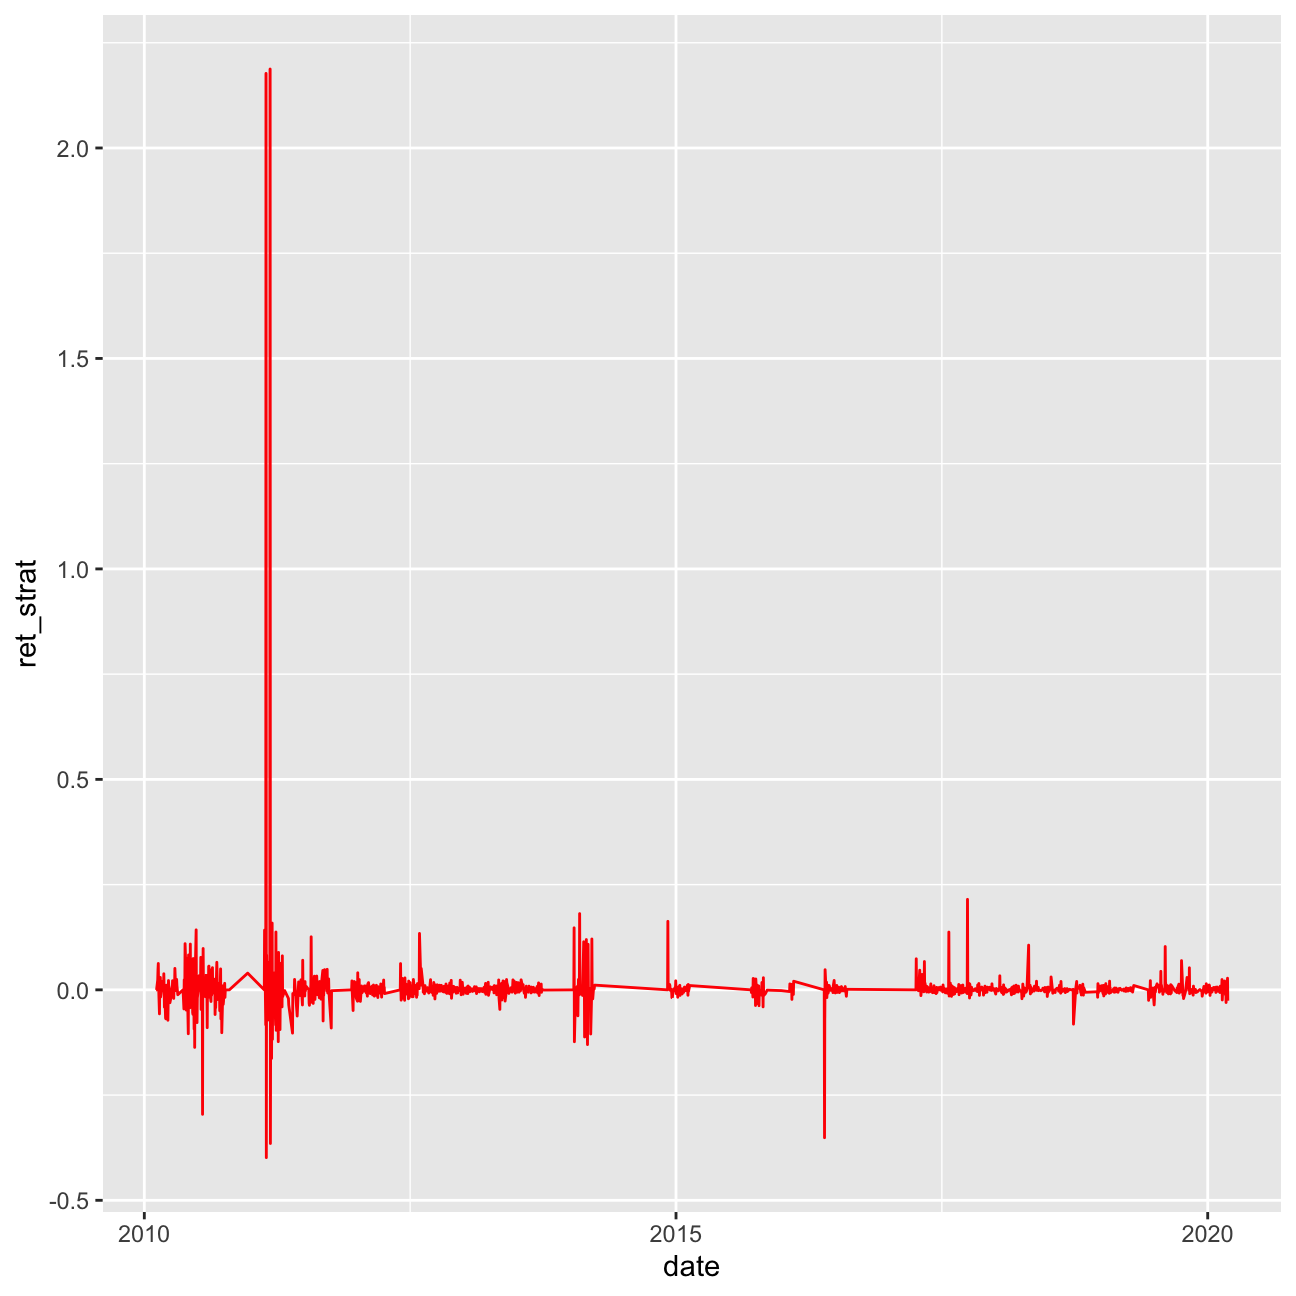
\includegraphics{DataAnalysisvF_files/figure-latex/unnamed-chunk-13-1} \end{center}

\begin{Shaded}
\begin{Highlighting}[]
\NormalTok{benchmark }\OperatorTok{\%\textgreater{}\%}
\StringTok{  }\KeywordTok{filter}\NormalTok{(description }\OperatorTok{==}\StringTok{ "SP\_500"}\NormalTok{) }\OperatorTok{\%\textgreater{}\%}
\StringTok{  }\KeywordTok{arrange}\NormalTok{(date) }\OperatorTok{\%\textgreater{}\%}
\StringTok{  }\KeywordTok{left\_join}\NormalTok{(SP\_initial, }\DataTypeTok{by =} \KeywordTok{c}\NormalTok{(}\StringTok{"description"}\NormalTok{, }\StringTok{"index"}\NormalTok{)) }\OperatorTok{\%\textgreater{}\%}
\StringTok{  }\KeywordTok{left\_join}\NormalTok{(acq\_tar2, }\DataTypeTok{by =} \StringTok{"date"}\NormalTok{) }\OperatorTok{\%\textgreater{}\%}
\StringTok{  }\KeywordTok{select}\NormalTok{(date, close, initial\_index, ret\_strat) }\OperatorTok{\%\textgreater{}\%}
\StringTok{  }\KeywordTok{mutate}\NormalTok{(}\DataTypeTok{index\_ret =}\NormalTok{ close}\OperatorTok{/}\KeywordTok{lag}\NormalTok{(close) }\OperatorTok{{-}}\StringTok{ }\DecValTok{1}\NormalTok{,}
         \DataTypeTok{cum\_index\_ret =}\NormalTok{ close}\OperatorTok{/}\NormalTok{initial\_index,}
         \DataTypeTok{ret\_strat\_adjusted =} \KeywordTok{ifelse}\NormalTok{(}\KeywordTok{is.na}\NormalTok{(ret\_strat), index\_ret, ret\_strat)) }\OperatorTok{\%\textgreater{}\%}
\StringTok{  }\KeywordTok{filter}\NormalTok{(date }\OperatorTok{\textgreater{}=}\StringTok{ "2015{-}01{-}01"}\NormalTok{) }\OperatorTok{\%\textgreater{}\%}
\StringTok{  }\KeywordTok{mutate}\NormalTok{(}\DataTypeTok{retplus1 =}\NormalTok{ ret\_strat\_adjusted }\OperatorTok{+}\StringTok{ }\DecValTok{1}\NormalTok{,}
    \DataTypeTok{cum\_ret\_strat =} \KeywordTok{cumprod}\NormalTok{(retplus1)) }\OperatorTok{\%\textgreater{}\%}
\StringTok{  }\KeywordTok{ggplot}\NormalTok{() }\OperatorTok{+}
\StringTok{  }\KeywordTok{geom\_line}\NormalTok{(}\KeywordTok{aes}\NormalTok{(}\DataTypeTok{x =}\NormalTok{ date, }\DataTypeTok{y =}\NormalTok{ cum\_index\_ret), }\DataTypeTok{colour =} \StringTok{"red"}\NormalTok{) }\OperatorTok{+}
\StringTok{  }\KeywordTok{geom\_line}\NormalTok{(}\KeywordTok{aes}\NormalTok{(}\DataTypeTok{x =}\NormalTok{ date, }\DataTypeTok{y =}\NormalTok{ cum\_ret\_strat), }\DataTypeTok{colour =} \StringTok{"green"}\NormalTok{) }\OperatorTok{+}
\StringTok{  }\KeywordTok{labs}\NormalTok{(}\DataTypeTok{subtitle =} \StringTok{"Cumulative Return Strategy vs Index"}\NormalTok{,}
       \DataTypeTok{title =} \StringTok{"Perfect Foresight Generates Above Market Returns"}\NormalTok{,}
       \DataTypeTok{y =} \StringTok{"Cumulative Return"}\NormalTok{,}
       \DataTypeTok{x =} \StringTok{"Day from initial investment"}\NormalTok{) }\OperatorTok{+}\StringTok{ }
\StringTok{  }\KeywordTok{theme\_economist\_white}\NormalTok{()}
\end{Highlighting}
\end{Shaded}

\begin{center}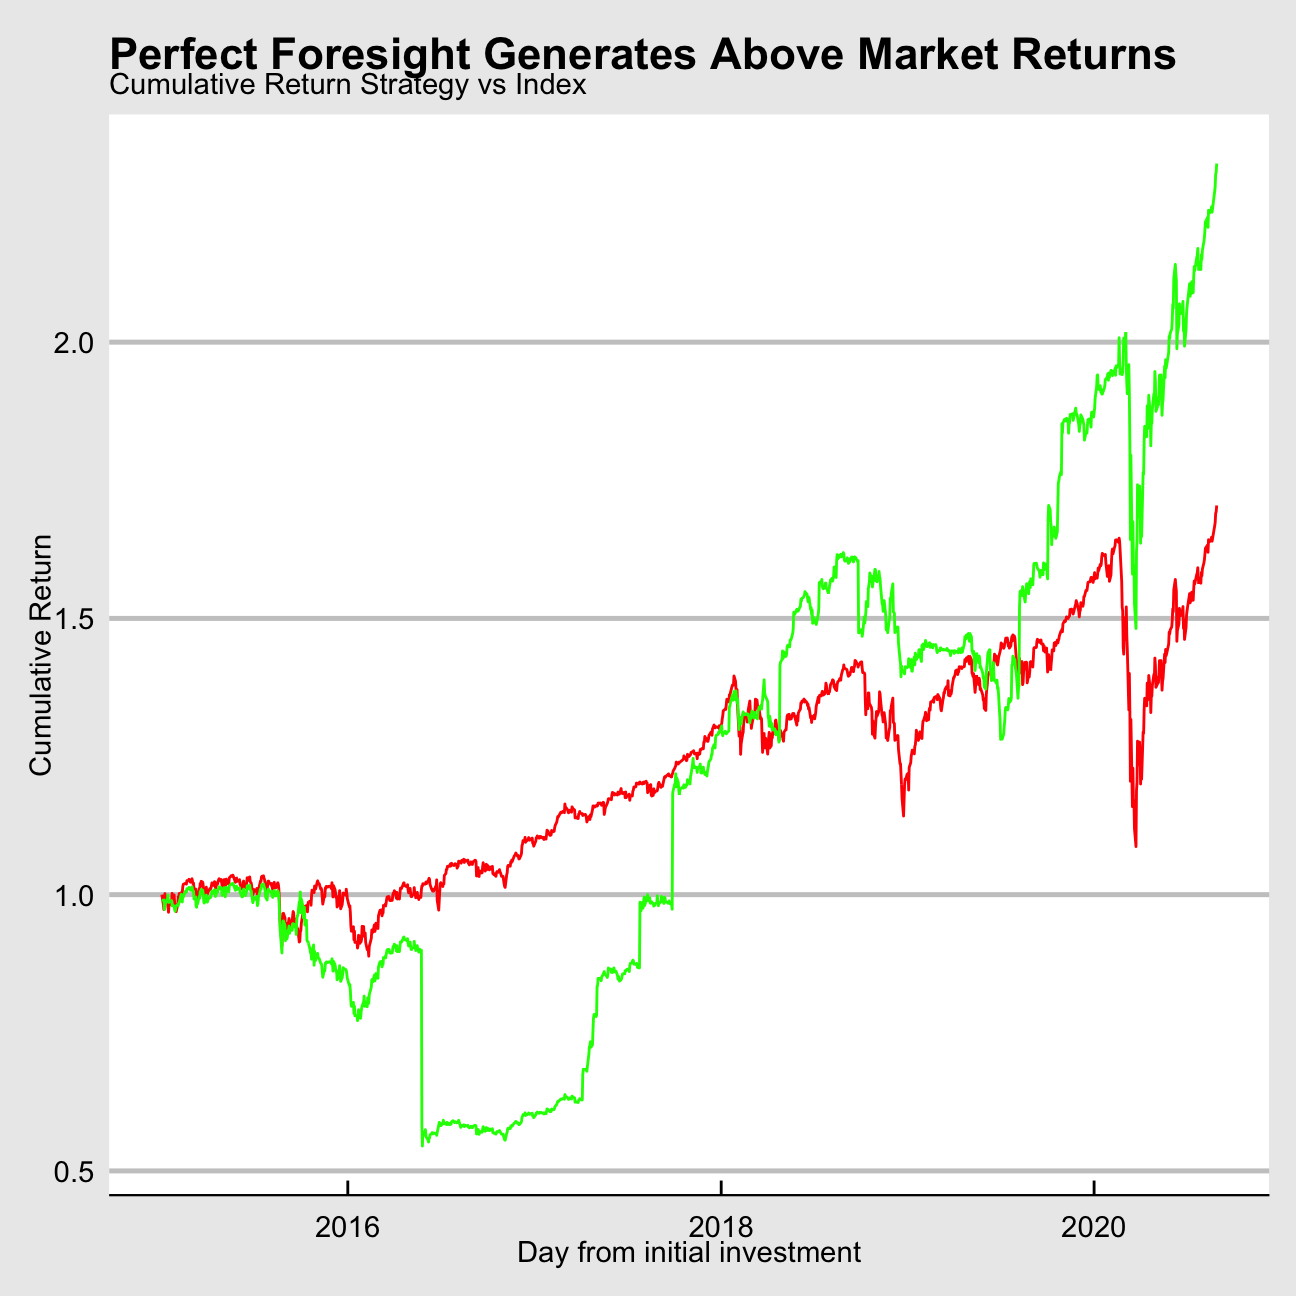
\includegraphics{DataAnalysisvF_files/figure-latex/unnamed-chunk-13-2} \end{center}

\begin{Shaded}
\begin{Highlighting}[]
\KeywordTok{ggsave}\NormalTok{(}\StringTok{"Cumulative Return Strategy vs Index.png"}\NormalTok{,}
       \DataTypeTok{plot =} \KeywordTok{last\_plot}\NormalTok{(),}
       \DataTypeTok{scale =} \DecValTok{1}\NormalTok{,}
       \DataTypeTok{width =} \DecValTok{20}\NormalTok{,}
       \DataTypeTok{height =} \DecValTok{15}\NormalTok{,}
       \DataTypeTok{units =} \StringTok{"cm"}\NormalTok{,}
       \DataTypeTok{dpi =} \DecValTok{300}\NormalTok{,}
       \DataTypeTok{limitsize =} \OtherTok{TRUE}\NormalTok{)}

\NormalTok{knitr}\OperatorTok{::}\KeywordTok{include\_graphics}\NormalTok{(here}\OperatorTok{::}\KeywordTok{here}\NormalTok{(}\StringTok{"Cumulative Return Strategy vs Index.png"}\NormalTok{), }\DataTypeTok{error =} \OtherTok{FALSE}\NormalTok{)}
\end{Highlighting}
\end{Shaded}

\begin{center}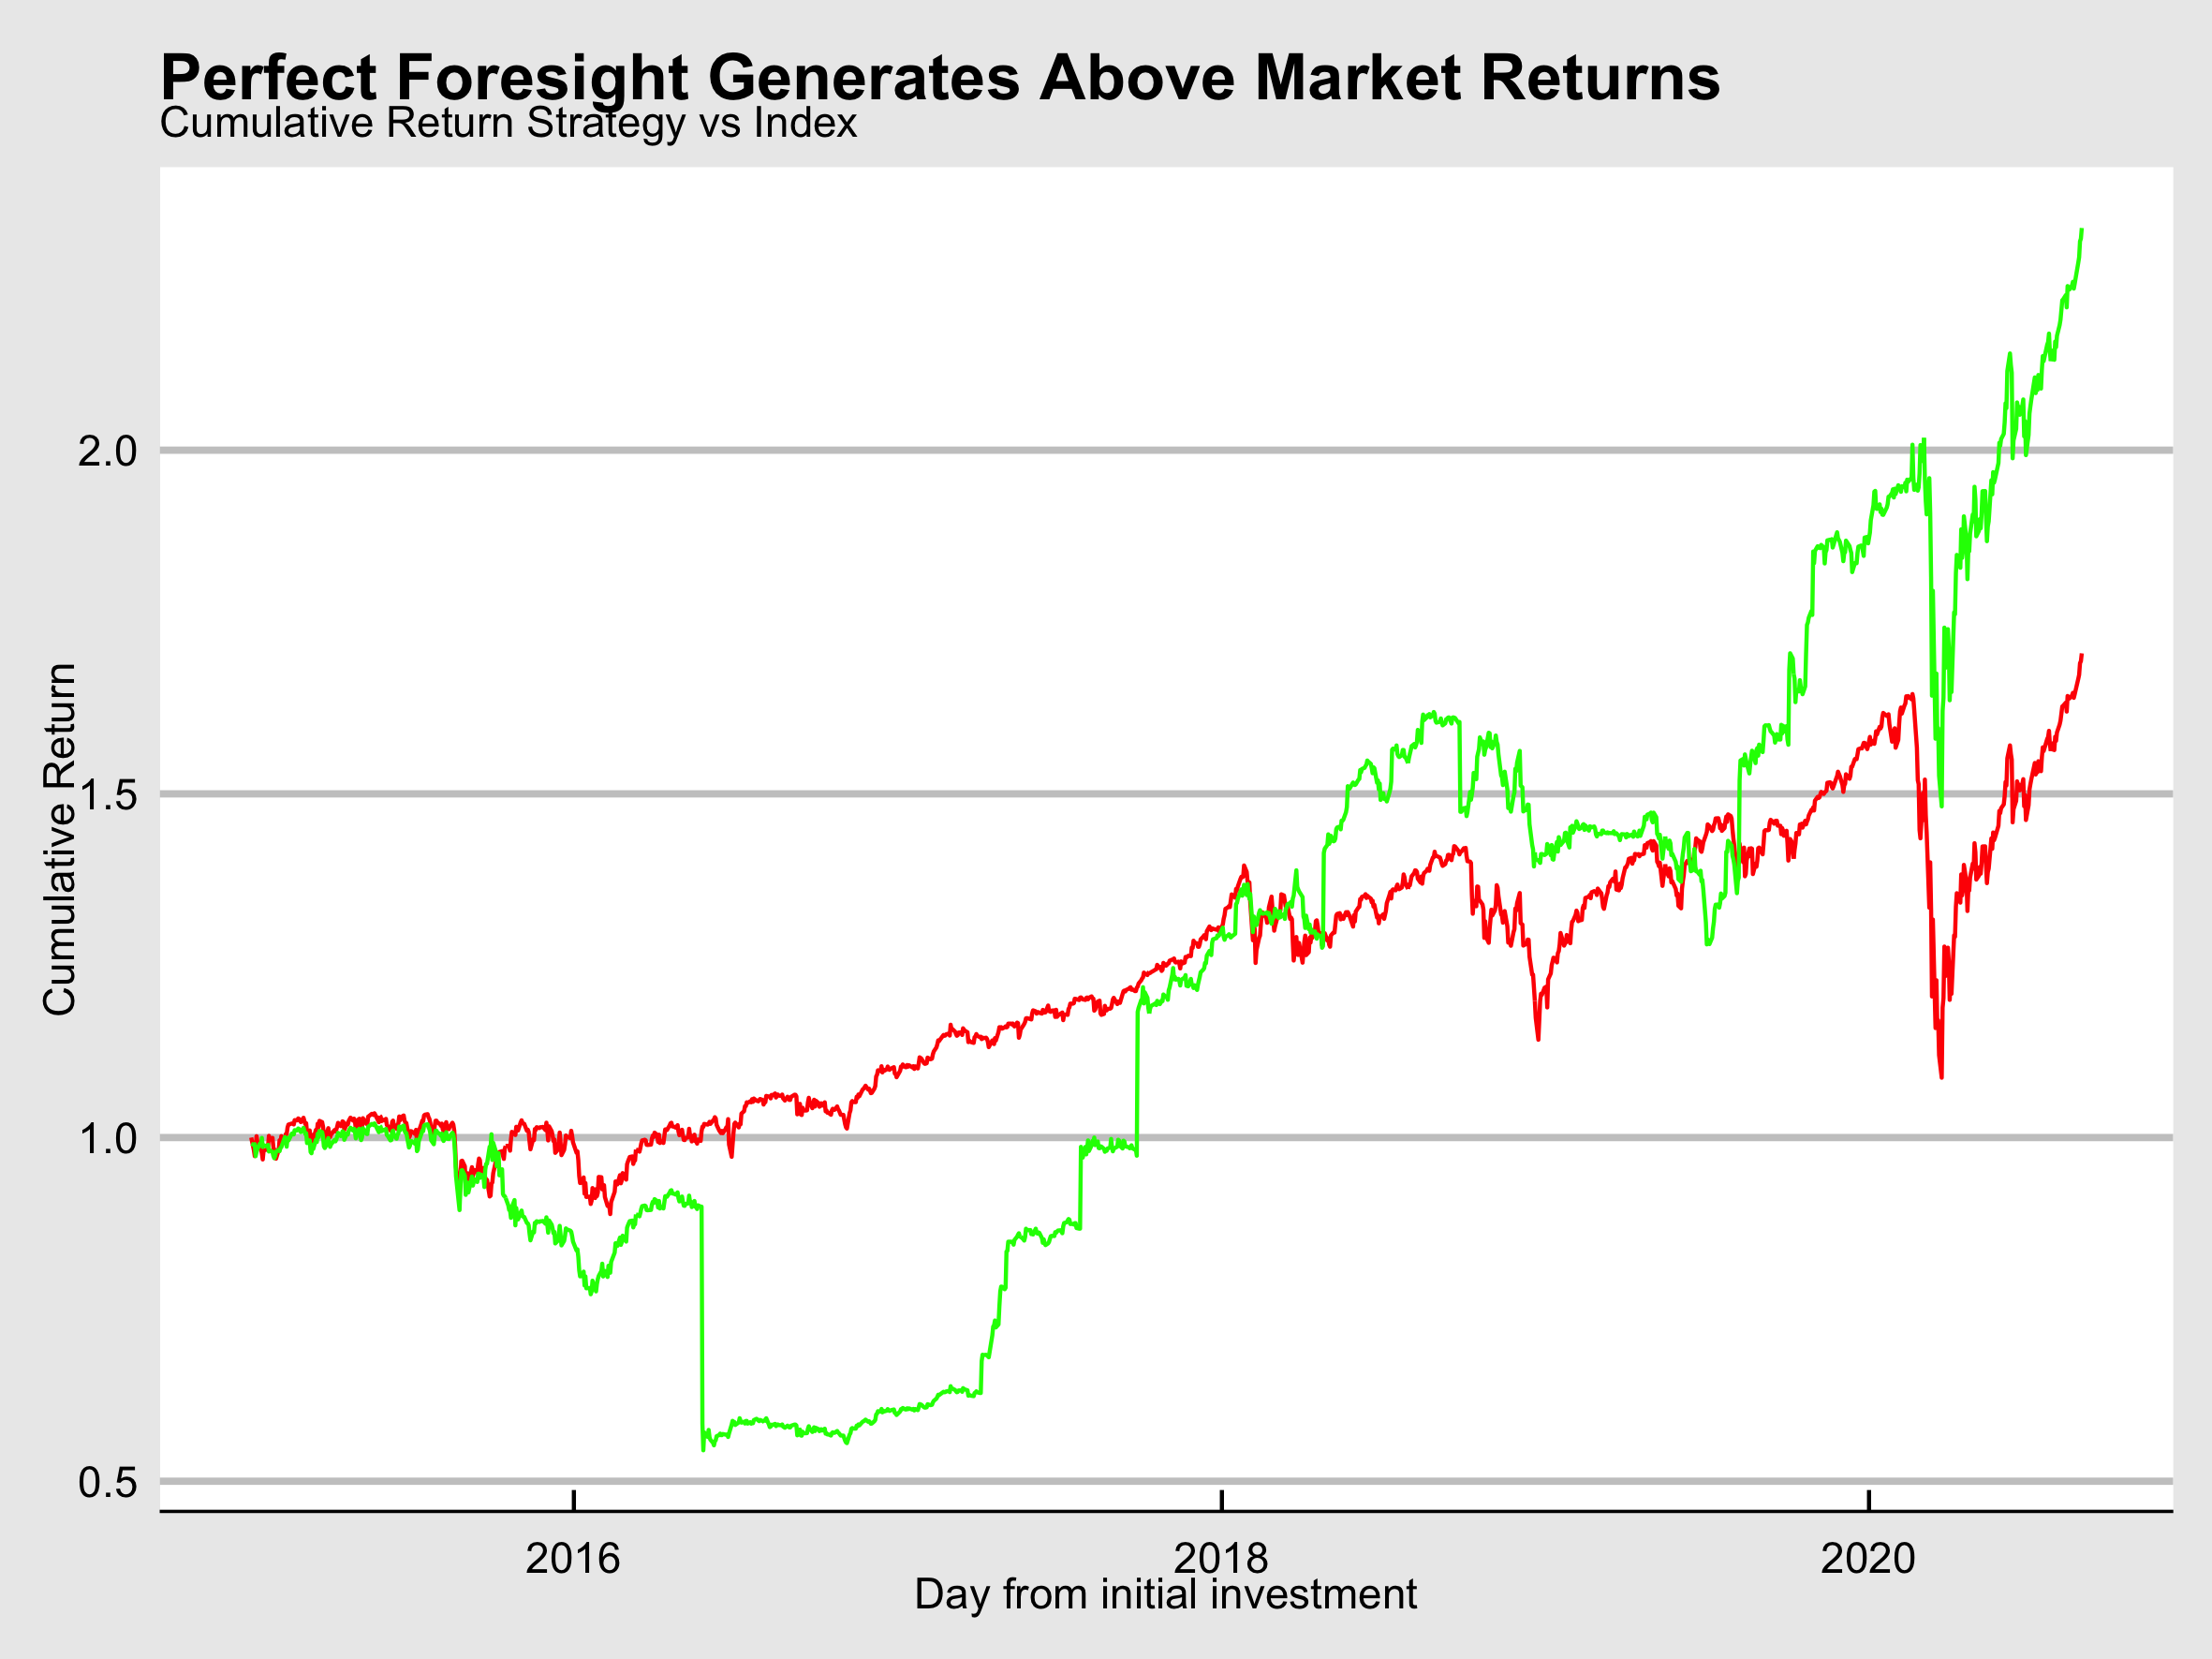
\includegraphics[width=32.81in]{/Users/leifbeckers/Desktop/LBS/Investment Fundamentals/Investment_Fundamentals/Cumulative Return Strategy vs Index} \end{center}

\hypertarget{risk-free-if-no-deal}{%
\subsubsection{Risk free if no deal}\label{risk-free-if-no-deal}}

\begin{Shaded}
\begin{Highlighting}[]
\NormalTok{benchmark }\OperatorTok{\%\textgreater{}\%}
\StringTok{  }\KeywordTok{filter}\NormalTok{(description }\OperatorTok{==}\StringTok{ "SP\_500"}\NormalTok{) }\OperatorTok{\%\textgreater{}\%}
\StringTok{  }\KeywordTok{arrange}\NormalTok{(date) }\OperatorTok{\%\textgreater{}\%}
\StringTok{  }\KeywordTok{left\_join}\NormalTok{(SP\_initial, }\DataTypeTok{by =} \KeywordTok{c}\NormalTok{(}\StringTok{"description"}\NormalTok{, }\StringTok{"index"}\NormalTok{)) }\OperatorTok{\%\textgreater{}\%}
\StringTok{  }\KeywordTok{left\_join}\NormalTok{(acq\_tar2, }\DataTypeTok{by =} \StringTok{"date"}\NormalTok{) }\OperatorTok{\%\textgreater{}\%}
\StringTok{  }\KeywordTok{left\_join}\NormalTok{(tbill, }\DataTypeTok{by =} \StringTok{"date"}\NormalTok{) }\OperatorTok{\%\textgreater{}\%}
\StringTok{  }\KeywordTok{select}\NormalTok{(date, close, initial\_index, ret\_strat, T\_bill\_d) }\OperatorTok{\%\textgreater{}\%}
\StringTok{  }\KeywordTok{mutate}\NormalTok{(}\DataTypeTok{index\_ret =}\NormalTok{ close}\OperatorTok{/}\KeywordTok{lag}\NormalTok{(close) }\OperatorTok{{-}}\StringTok{ }\DecValTok{1}\NormalTok{,}
         \DataTypeTok{cum\_index\_ret =}\NormalTok{ close}\OperatorTok{/}\NormalTok{initial\_index,}
         \DataTypeTok{ret\_strat\_adjusted =} \KeywordTok{ifelse}\NormalTok{(}\KeywordTok{is.na}\NormalTok{(ret\_strat), T\_bill\_d, ret\_strat)) }\OperatorTok{\%\textgreater{}\%}
\StringTok{  }\KeywordTok{filter}\NormalTok{(date }\OperatorTok{\textgreater{}=}\StringTok{ "2014{-}05{-}01"}\NormalTok{) }\OperatorTok{\%\textgreater{}\%}
\StringTok{  }\KeywordTok{mutate}\NormalTok{(}\DataTypeTok{retplus1 =}\NormalTok{ ret\_strat\_adjusted }\OperatorTok{+}\StringTok{ }\DecValTok{1}\NormalTok{,}
    \DataTypeTok{cum\_ret\_strat =} \KeywordTok{cumprod}\NormalTok{(retplus1)) }\OperatorTok{\%\textgreater{}\%}
\StringTok{  }\KeywordTok{ggplot}\NormalTok{() }\OperatorTok{+}
\StringTok{  }\KeywordTok{geom\_line}\NormalTok{(}\KeywordTok{aes}\NormalTok{(}\DataTypeTok{x =}\NormalTok{ date, }\DataTypeTok{y =}\NormalTok{ cum\_index\_ret), }\DataTypeTok{colour =} \StringTok{"red"}\NormalTok{) }\OperatorTok{+}
\StringTok{  }\KeywordTok{geom\_line}\NormalTok{(}\KeywordTok{aes}\NormalTok{(}\DataTypeTok{x =}\NormalTok{ date, }\DataTypeTok{y =}\NormalTok{ cum\_ret\_strat), }\DataTypeTok{colour =} \StringTok{"green"}\NormalTok{) }\OperatorTok{+}
\StringTok{  }\KeywordTok{labs}\NormalTok{(}\DataTypeTok{subtitle =} \StringTok{"Cumulative Return Strategy vs Index"}\NormalTok{,}
       \DataTypeTok{title =} \StringTok{"Perfect Foresight Generates Above Market Returns"}\NormalTok{,}
       \DataTypeTok{y =} \StringTok{"Cumulative Return"}\NormalTok{,}
       \DataTypeTok{x =} \StringTok{"Day from initial investment"}\NormalTok{) }\OperatorTok{+}\StringTok{ }
\StringTok{  }\KeywordTok{theme\_economist\_white}\NormalTok{()}
\end{Highlighting}
\end{Shaded}

\begin{center}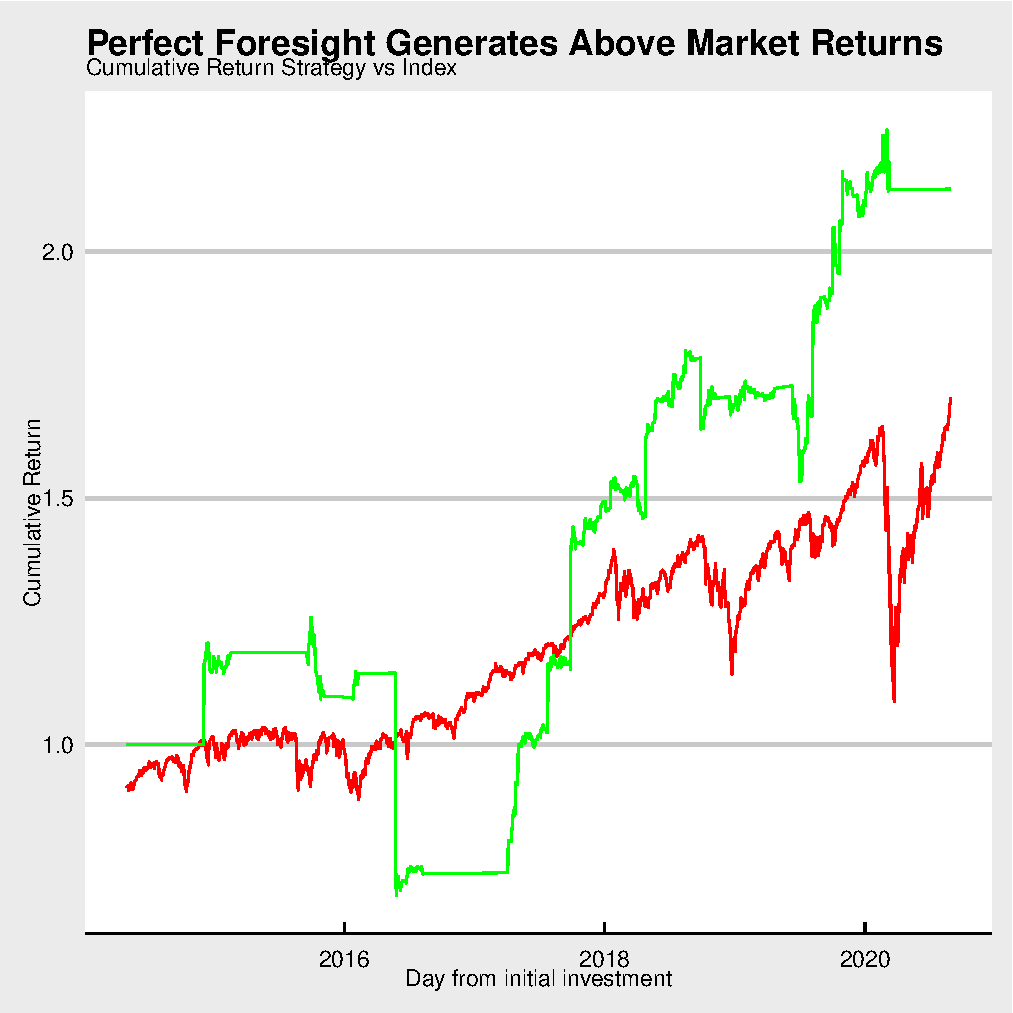
\includegraphics{DataAnalysisvF_files/figure-latex/unnamed-chunk-14-1} \end{center}

\hypertarget{capm}{%
\subsection{CAPM}\label{capm}}

\begin{Shaded}
\begin{Highlighting}[]
\NormalTok{benchmarkSP \textless{}{-}}\StringTok{ }\NormalTok{benchmark }\OperatorTok{\%\textgreater{}\%}
\StringTok{  }\KeywordTok{filter}\NormalTok{(description }\OperatorTok{==}\StringTok{ "SP\_500"}\NormalTok{) }\OperatorTok{\%\textgreater{}\%}
\StringTok{  }\KeywordTok{pivot\_wider}\NormalTok{(}\DataTypeTok{values\_from =}\NormalTok{ index\_return, }\DataTypeTok{names\_from =}\NormalTok{ description) }\OperatorTok{\%\textgreater{}\%}
\StringTok{  }\KeywordTok{select}\NormalTok{(date, SP\_}\DecValTok{500}\NormalTok{)}


\NormalTok{CAPM \textless{}{-}}\StringTok{ }\NormalTok{acq\_tar }\OperatorTok{\%\textgreater{}\%}
\StringTok{  }\KeywordTok{filter}\NormalTok{(period }\OperatorTok{\textless{}=}\StringTok{ }\DecValTok{20}\NormalTok{) }\OperatorTok{\%\textgreater{}\%}\StringTok{ }
\StringTok{  }\KeywordTok{left\_join}\NormalTok{(tbill, }\DataTypeTok{by =} \StringTok{"date"}\NormalTok{) }\OperatorTok{\%\textgreater{}\%}
\StringTok{  }\KeywordTok{left\_join}\NormalTok{(benchmarkSP, }\DataTypeTok{by =} \StringTok{"date"}\NormalTok{) }\OperatorTok{\%\textgreater{}\%}\StringTok{ }
\StringTok{  }\KeywordTok{filter}\NormalTok{(}\OperatorTok{!}\KeywordTok{is.na}\NormalTok{(ret\_combined)) }\OperatorTok{\%\textgreater{}\%}\StringTok{ }
\StringTok{  }\KeywordTok{mutate}\NormalTok{(}\DataTypeTok{Rm\_Rf =}\NormalTok{ SP\_}\DecValTok{500} \OperatorTok{{-}}\StringTok{ }\NormalTok{T\_bill\_d,}
         \DataTypeTok{Rs\_Rf =}\NormalTok{ ret\_combined }\OperatorTok{{-}}\StringTok{ }\NormalTok{T\_bill\_d) }\OperatorTok{\%\textgreater{}\%}\StringTok{  }\CommentTok{\# CAN MUTATE RET\_Strat = S\&P/TBill if return = NA, then use that to replace ret\_combined here}
\StringTok{  }\KeywordTok{drop\_na}\NormalTok{(Rm\_Rf, Rs\_Rf) }\OperatorTok{\%\textgreater{}\%}
\StringTok{  }\KeywordTok{filter}\NormalTok{(}\OperatorTok{!}\KeywordTok{is.infinite}\NormalTok{(Rs\_Rf))}

\KeywordTok{ggplot}\NormalTok{(CAPM, }\KeywordTok{aes}\NormalTok{(}\DataTypeTok{x =}\NormalTok{ Rm\_Rf, }\DataTypeTok{y =}\NormalTok{ Rs\_Rf, }\DataTypeTok{na.rm =} \OtherTok{TRUE}\NormalTok{)) }\OperatorTok{+}
\StringTok{  }\KeywordTok{geom\_point}\NormalTok{() }\OperatorTok{+}
\StringTok{  }\KeywordTok{geom\_smooth}\NormalTok{(}\DataTypeTok{method =}\NormalTok{ lm)  }\OperatorTok{+}
\StringTok{  }\KeywordTok{ylim}\NormalTok{(}\OperatorTok{{-}}\DecValTok{1}\NormalTok{,}\DecValTok{1}\NormalTok{) }\OperatorTok{+}
\StringTok{  }\KeywordTok{labs}\NormalTok{(}\DataTypeTok{subtitle =} \StringTok{"Excess Returns of Startegy vs Market Benchmark (scale ignoring 2 outliers)"}\NormalTok{,}
       \DataTypeTok{title =} \StringTok{"Regression shows minimal positive Alpha and Beta for daily returns"}\NormalTok{,}
       \DataTypeTok{y =} \StringTok{"Excess Return Strategy"}\NormalTok{,}
       \DataTypeTok{x =} \StringTok{"Excess Return Benchmark"}\NormalTok{) }\OperatorTok{+}\StringTok{ }
\StringTok{  }\KeywordTok{theme\_economist\_white}\NormalTok{()}
\end{Highlighting}
\end{Shaded}

\begin{center}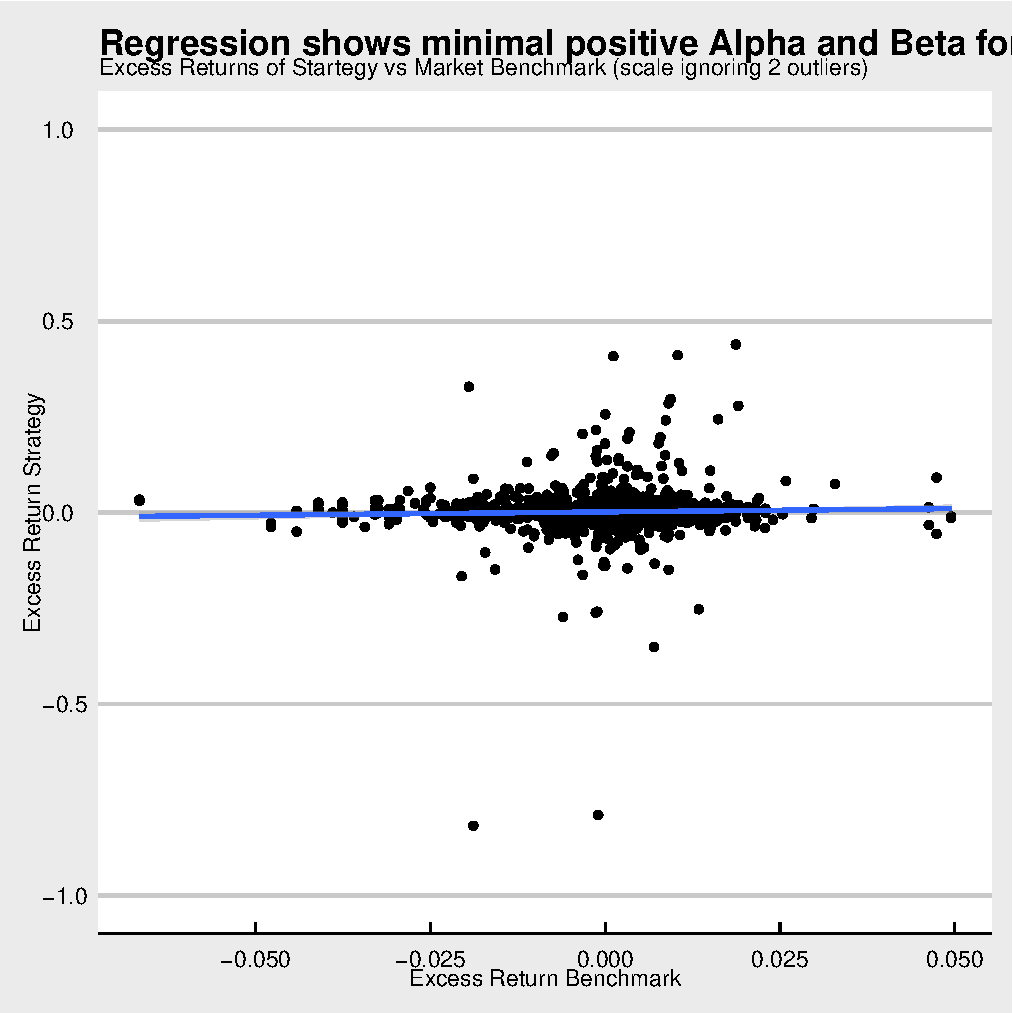
\includegraphics{DataAnalysisvF_files/figure-latex/unnamed-chunk-15-1} \end{center}

\begin{Shaded}
\begin{Highlighting}[]
\KeywordTok{ggsave}\NormalTok{(}\StringTok{"Excess Returns of Startegy vs Market Benchmark.png"}\NormalTok{,}
       \DataTypeTok{plot =} \KeywordTok{last\_plot}\NormalTok{(),}
       \DataTypeTok{scale =} \DecValTok{1}\NormalTok{,}
       \DataTypeTok{width =} \DecValTok{25}\NormalTok{,}
       \DataTypeTok{height =} \DecValTok{15}\NormalTok{,}
       \DataTypeTok{units =} \StringTok{"cm"}\NormalTok{,}
       \DataTypeTok{dpi =} \DecValTok{300}\NormalTok{,}
       \DataTypeTok{limitsize =} \OtherTok{TRUE}\NormalTok{)}

\NormalTok{knitr}\OperatorTok{::}\KeywordTok{include\_graphics}\NormalTok{(here}\OperatorTok{::}\KeywordTok{here}\NormalTok{(}\StringTok{"Excess Returns of Startegy vs Market Benchmark.png"}\NormalTok{), }\DataTypeTok{error =} \OtherTok{FALSE}\NormalTok{)}
\end{Highlighting}
\end{Shaded}

\begin{center}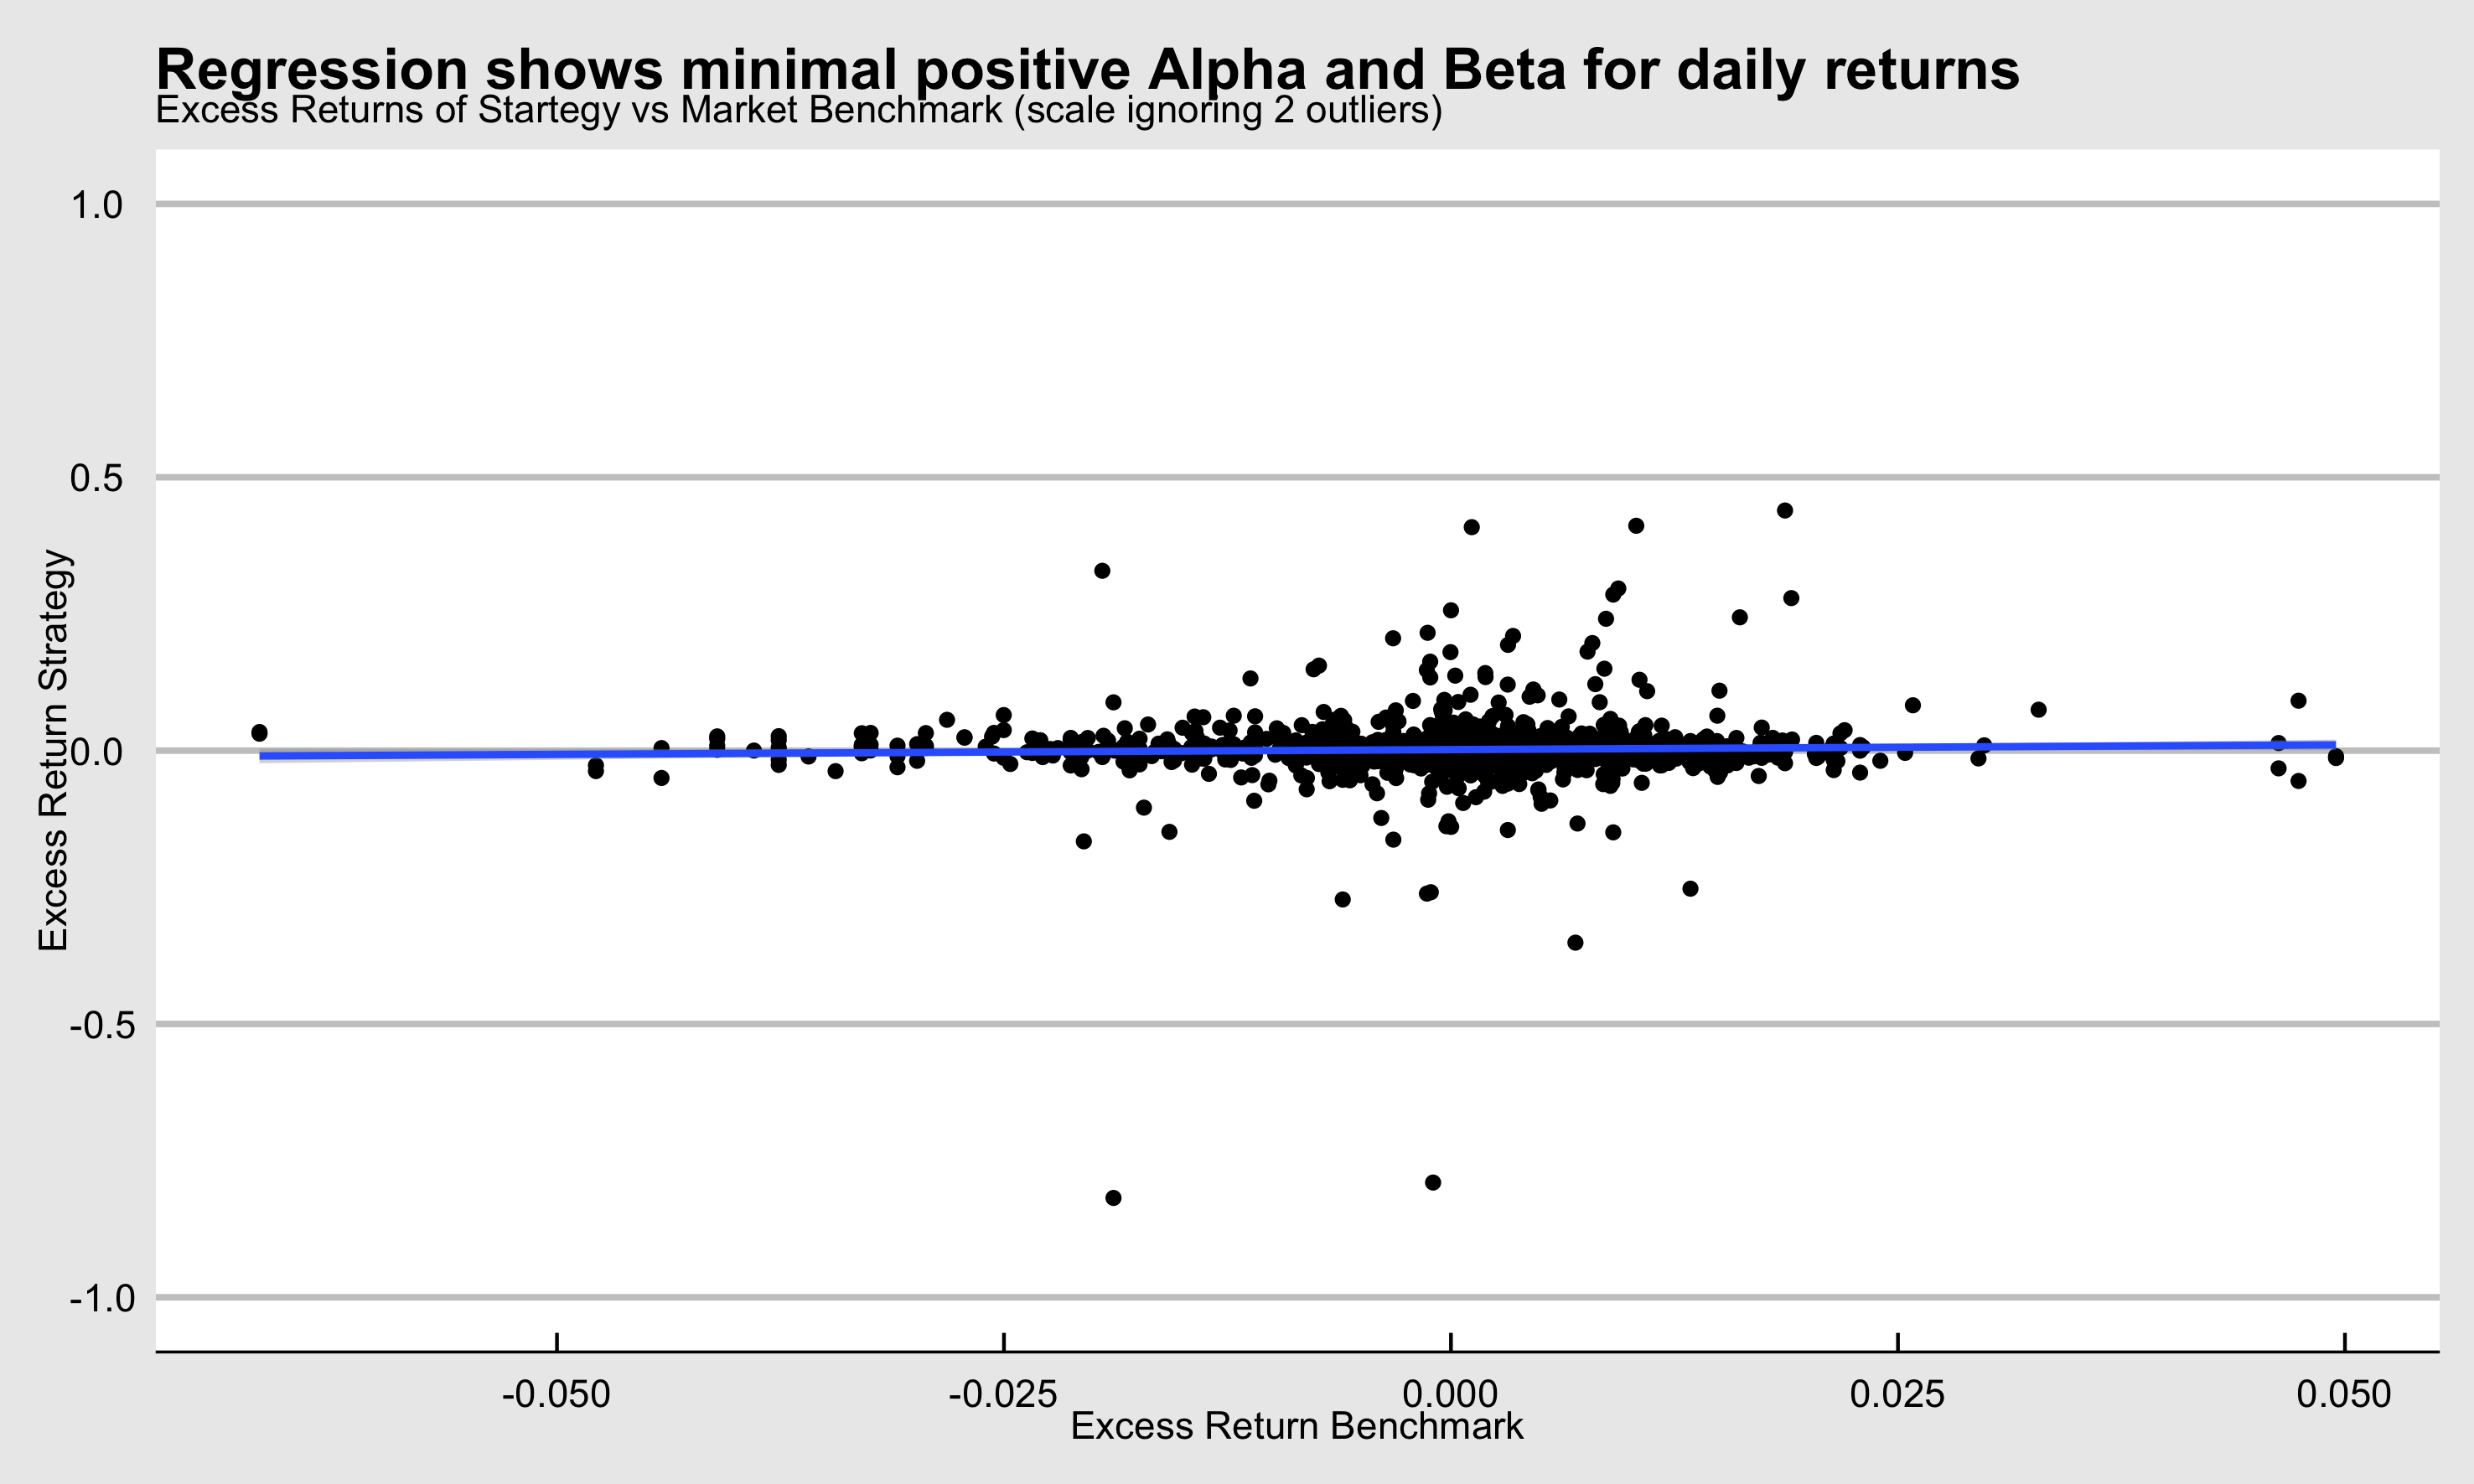
\includegraphics[width=41in]{/Users/leifbeckers/Desktop/LBS/Investment Fundamentals/Investment_Fundamentals/Excess Returns of Startegy vs Market Benchmark} \end{center}

\begin{Shaded}
\begin{Highlighting}[]
\NormalTok{CAPM\_regression \textless{}{-}}\StringTok{ }\KeywordTok{lm}\NormalTok{(Rs\_Rf }\OperatorTok{\textasciitilde{}}\StringTok{ }\NormalTok{Rm\_Rf, }\DataTypeTok{data =}\NormalTok{ CAPM, }\DataTypeTok{na.rm =}\OtherTok{TRUE}\NormalTok{)}

\NormalTok{CAPM\_regression}
\end{Highlighting}
\end{Shaded}

\begin{verbatim}
## 
## Call:
## lm(formula = Rs_Rf ~ Rm_Rf, data = CAPM, na.rm = TRUE)
## 
## Coefficients:
## (Intercept)        Rm_Rf  
##    0.005822     0.000526
\end{verbatim}

\begin{Shaded}
\begin{Highlighting}[]
\KeywordTok{huxreg}\NormalTok{(CAPM\_regression,}
       \DataTypeTok{statistics =} \KeywordTok{c}\NormalTok{(}\StringTok{\textquotesingle{}\#observations\textquotesingle{}}\NormalTok{ =}\StringTok{ \textquotesingle{}nobs\textquotesingle{}}\NormalTok{, }
                      \StringTok{\textquotesingle{}R squared\textquotesingle{}}\NormalTok{ =}\StringTok{ \textquotesingle{}r.squared\textquotesingle{}}\NormalTok{, }
                      \StringTok{\textquotesingle{}Adj. R Squared\textquotesingle{}}\NormalTok{ =}\StringTok{ \textquotesingle{}adj.r.squared\textquotesingle{}}\NormalTok{, }
                      \StringTok{\textquotesingle{}Residual SE\textquotesingle{}}\NormalTok{ =}\StringTok{ \textquotesingle{}sigma\textquotesingle{}}\NormalTok{), }
       \DataTypeTok{bold\_signif =} \FloatTok{0.05}\NormalTok{, }
       \DataTypeTok{stars =} \OtherTok{NULL}
\NormalTok{)}
\end{Highlighting}
\end{Shaded}

 
  \providecommand{\huxb}[2]{\arrayrulecolor[RGB]{#1}\global\arrayrulewidth=#2pt}
  \providecommand{\huxvb}[2]{\color[RGB]{#1}\vrule width #2pt}
  \providecommand{\huxtpad}[1]{\rule{0pt}{#1}}
  \providecommand{\huxbpad}[1]{\rule[-#1]{0pt}{#1}}

\begin{table}[ht]
\begin{centerbox}
\begin{threeparttable}
 \label{tab:unnamed-chunk-15}
\setlength{\tabcolsep}{0pt}
\begin{tabular}{l l}


\hhline{>{\huxb{0, 0, 0}{0.8}}->{\huxb{0, 0, 0}{0.8}}-}
\arrayrulecolor{black}

\multicolumn{1}{!{\huxvb{0, 0, 0}{0}}c!{\huxvb{0, 0, 0}{0}}}{\huxtpad{6pt + 1em}\centering \hspace{6pt}  \hspace{6pt}\huxbpad{6pt}} &
\multicolumn{1}{c!{\huxvb{0, 0, 0}{0}}}{\huxtpad{6pt + 1em}\centering \hspace{6pt} (1) \hspace{6pt}\huxbpad{6pt}} \tabularnewline[-0.5pt]


\hhline{>{\huxb{255, 255, 255}{0.4}}->{\huxb{0, 0, 0}{0.4}}-}
\arrayrulecolor{black}

\multicolumn{1}{!{\huxvb{0, 0, 0}{0}}l!{\huxvb{0, 0, 0}{0}}}{\huxtpad{6pt + 1em}\raggedright \hspace{6pt} (Intercept) \hspace{6pt}\huxbpad{6pt}} &
\multicolumn{1}{r!{\huxvb{0, 0, 0}{0}}}{\huxtpad{6pt + 1em}\raggedleft \hspace{6pt} \textbf{0.006~} \hspace{6pt}\huxbpad{6pt}} \tabularnewline[-0.5pt]


\hhline{}
\arrayrulecolor{black}

\multicolumn{1}{!{\huxvb{0, 0, 0}{0}}l!{\huxvb{0, 0, 0}{0}}}{\huxtpad{6pt + 1em}\raggedright \hspace{6pt}  \hspace{6pt}\huxbpad{6pt}} &
\multicolumn{1}{r!{\huxvb{0, 0, 0}{0}}}{\huxtpad{6pt + 1em}\raggedleft \hspace{6pt} \textbf{(0.003)} \hspace{6pt}\huxbpad{6pt}} \tabularnewline[-0.5pt]


\hhline{}
\arrayrulecolor{black}

\multicolumn{1}{!{\huxvb{0, 0, 0}{0}}l!{\huxvb{0, 0, 0}{0}}}{\huxtpad{6pt + 1em}\raggedright \hspace{6pt} Rm\_Rf \hspace{6pt}\huxbpad{6pt}} &
\multicolumn{1}{r!{\huxvb{0, 0, 0}{0}}}{\huxtpad{6pt + 1em}\raggedleft \hspace{6pt} 0.001~ \hspace{6pt}\huxbpad{6pt}} \tabularnewline[-0.5pt]


\hhline{}
\arrayrulecolor{black}

\multicolumn{1}{!{\huxvb{0, 0, 0}{0}}l!{\huxvb{0, 0, 0}{0}}}{\huxtpad{6pt + 1em}\raggedright \hspace{6pt}  \hspace{6pt}\huxbpad{6pt}} &
\multicolumn{1}{r!{\huxvb{0, 0, 0}{0}}}{\huxtpad{6pt + 1em}\raggedleft \hspace{6pt} (0.311) \hspace{6pt}\huxbpad{6pt}} \tabularnewline[-0.5pt]


\hhline{>{\huxb{255, 255, 255}{0.4}}->{\huxb{0, 0, 0}{0.4}}-}
\arrayrulecolor{black}

\multicolumn{1}{!{\huxvb{0, 0, 0}{0}}l!{\huxvb{0, 0, 0}{0}}}{\huxtpad{6pt + 1em}\raggedright \hspace{6pt} \#observations \hspace{6pt}\huxbpad{6pt}} &
\multicolumn{1}{r!{\huxvb{0, 0, 0}{0}}}{\huxtpad{6pt + 1em}\raggedleft \hspace{6pt} 2213~~~~~ \hspace{6pt}\huxbpad{6pt}} \tabularnewline[-0.5pt]


\hhline{}
\arrayrulecolor{black}

\multicolumn{1}{!{\huxvb{0, 0, 0}{0}}l!{\huxvb{0, 0, 0}{0}}}{\huxtpad{6pt + 1em}\raggedright \hspace{6pt} R squared \hspace{6pt}\huxbpad{6pt}} &
\multicolumn{1}{r!{\huxvb{0, 0, 0}{0}}}{\huxtpad{6pt + 1em}\raggedleft \hspace{6pt} 0.000~ \hspace{6pt}\huxbpad{6pt}} \tabularnewline[-0.5pt]


\hhline{}
\arrayrulecolor{black}

\multicolumn{1}{!{\huxvb{0, 0, 0}{0}}l!{\huxvb{0, 0, 0}{0}}}{\huxtpad{6pt + 1em}\raggedright \hspace{6pt} Adj. R Squared \hspace{6pt}\huxbpad{6pt}} &
\multicolumn{1}{r!{\huxvb{0, 0, 0}{0}}}{\huxtpad{6pt + 1em}\raggedleft \hspace{6pt} -0.000~ \hspace{6pt}\huxbpad{6pt}} \tabularnewline[-0.5pt]


\hhline{}
\arrayrulecolor{black}

\multicolumn{1}{!{\huxvb{0, 0, 0}{0}}l!{\huxvb{0, 0, 0}{0}}}{\huxtpad{6pt + 1em}\raggedright \hspace{6pt} Residual SE \hspace{6pt}\huxbpad{6pt}} &
\multicolumn{1}{r!{\huxvb{0, 0, 0}{0}}}{\huxtpad{6pt + 1em}\raggedleft \hspace{6pt} 0.139~ \hspace{6pt}\huxbpad{6pt}} \tabularnewline[-0.5pt]


\hhline{>{\huxb{0, 0, 0}{0.8}}->{\huxb{0, 0, 0}{0.8}}-}
\arrayrulecolor{black}
\end{tabular}
\end{threeparttable}\par\end{centerbox}

\end{table}
 

\begin{Shaded}
\begin{Highlighting}[]
\KeywordTok{msummary}\NormalTok{(CAPM\_regression)}
\end{Highlighting}
\end{Shaded}

\begin{verbatim}
##             Estimate Std. Error t value Pr(>|t|)  
## (Intercept) 0.005822   0.002950    1.97    0.049 *
## Rm_Rf       0.000526   0.311403    0.00    0.999  
## 
## Residual standard error: 0.139 on 2211 degrees of freedom
## Multiple R-squared:  1.29e-09,   Adjusted R-squared:  -0.000452 
## F-statistic: 2.85e-06 on 1 and 2211 DF,  p-value: 0.999
\end{verbatim}

----- END OF ANALYSIS USED IN PAPER --------

\hypertarget{unsused-calculations}{%
\subsubsection{Unsused Calculations}\label{unsused-calculations}}

The remainder of this document are conducted analyses that were chosen
not to report on in the project.

TRADE AFTER ANNOUNCEMENT DATE - SHOULD USE CLOSING PRICES HERE

\begin{Shaded}
\begin{Highlighting}[]
\CommentTok{\# Reformat acquirer data}
\NormalTok{stock\_data\_acquirer\_v2 \textless{}{-}}\StringTok{ }\NormalTok{acquirer\_raw }\OperatorTok{\%\textgreater{}\%}
\StringTok{  }\KeywordTok{group\_by}\NormalTok{(acquirer) }\OperatorTok{\%\textgreater{}\%}\StringTok{ }
\StringTok{  }\KeywordTok{mutate}\NormalTok{(}\DataTypeTok{close\_acquirer =} \KeywordTok{sprintf}\NormalTok{(}\StringTok{"\%.2f"}\NormalTok{, close, }\DataTypeTok{na.rm =} \OtherTok{TRUE}\NormalTok{)) }\OperatorTok{\%\textgreater{}\%}
\StringTok{  }\KeywordTok{select}\NormalTok{(acquirer, date, close\_acquirer)}
\end{Highlighting}
\end{Shaded}

\begin{Shaded}
\begin{Highlighting}[]
\CommentTok{\# Reformat target data}
\NormalTok{stock\_data\_target\_v2 \textless{}{-}}\StringTok{ }\NormalTok{target\_raw }\OperatorTok{\%\textgreater{}\%}
\StringTok{  }\KeywordTok{group\_by}\NormalTok{(target) }\OperatorTok{\%\textgreater{}\%}\StringTok{ }
\StringTok{  }\KeywordTok{mutate}\NormalTok{(}\DataTypeTok{close\_target =} \KeywordTok{sprintf}\NormalTok{(}\StringTok{"\%.2f"}\NormalTok{, close, }\DataTypeTok{na.rm =} \OtherTok{TRUE}\NormalTok{)) }\OperatorTok{\%\textgreater{}\%}
\StringTok{  }\KeywordTok{select}\NormalTok{(target, date, close\_target)}
\end{Highlighting}
\end{Shaded}

\begin{Shaded}
\begin{Highlighting}[]
\NormalTok{acq\_tar \textless{}{-}}\StringTok{ }\NormalTok{stocks2 }\OperatorTok{\%\textgreater{}\%}
\StringTok{  }
\StringTok{  }\CommentTok{\#Add acquirer data}
\StringTok{  }\KeywordTok{left\_join}\NormalTok{(stock\_data\_acquirer, }\DataTypeTok{by =} \KeywordTok{c}\NormalTok{(}\StringTok{"acquirer"}\NormalTok{)) }\OperatorTok{\%\textgreater{}\%}
\StringTok{  }\KeywordTok{distinct}\NormalTok{(DealID, date, }\DataTypeTok{.keep\_all =}\NormalTok{ T) }\OperatorTok{\%\textgreater{}\%}\StringTok{ }
\StringTok{  }\KeywordTok{mutate}\NormalTok{(}\DataTypeTok{announce\_date =} \KeywordTok{as.Date}\NormalTok{(announce\_date,}\StringTok{"\%Y{-}\%m{-}\%d"}\NormalTok{, }\DataTypeTok{tz =} \StringTok{"America/New\_York"}\NormalTok{),}
         \DataTypeTok{close\_date =} \KeywordTok{as.Date}\NormalTok{(close\_date,}\StringTok{"\%Y{-}\%m{-}\%d"}\NormalTok{, }\DataTypeTok{tz =} \StringTok{"America/New\_York"}\NormalTok{),}
         \DataTypeTok{standard\_date =}\NormalTok{ date }\OperatorTok{{-}}\StringTok{ }\NormalTok{announce\_date,}
         \DataTypeTok{standard\_date2 =} \KeywordTok{lead}\NormalTok{(standard\_date, }\DataTypeTok{n =}\NormalTok{ 2L)) }\OperatorTok{\%\textgreater{}\%}\StringTok{ }
\StringTok{  }\KeywordTok{group\_by}\NormalTok{(DealID) }\OperatorTok{\%\textgreater{}\%}\StringTok{ }
\StringTok{  }\KeywordTok{filter}\NormalTok{(standard\_date }\OperatorTok{\textgreater{}=}\StringTok{ }\DecValTok{{-}2}\NormalTok{,}
\NormalTok{         date }\OperatorTok{\textless{}=}\StringTok{ }\NormalTok{close\_date) }\OperatorTok{\%\textgreater{}\%}\StringTok{ }
\StringTok{  }\KeywordTok{mutate}\NormalTok{(}\DataTypeTok{period =} \KeywordTok{row\_number}\NormalTok{(),}
         \DataTypeTok{period =}\NormalTok{ period }\OperatorTok{+}\StringTok{ }\KeywordTok{as.numeric}\NormalTok{(}\KeywordTok{time\_length}\NormalTok{( }\KeywordTok{min}\NormalTok{(standard\_date), }\StringTok{"days"}\NormalTok{)) }\DecValTok{{-}1}\NormalTok{) }\OperatorTok{\%\textgreater{}\%}\StringTok{ }

\StringTok{  }\KeywordTok{left\_join}\NormalTok{(stock\_data\_target, }\DataTypeTok{by =} \KeywordTok{c}\NormalTok{(}\StringTok{"target"}\NormalTok{, }\StringTok{"date"}\NormalTok{)) }\OperatorTok{\%\textgreater{}\%}
\StringTok{  }\KeywordTok{drop\_na}\NormalTok{(close\_target) }\OperatorTok{\%\textgreater{}\%}

\StringTok{  }\KeywordTok{group\_by}\NormalTok{(DealID) }\OperatorTok{\%\textgreater{}\%}
\StringTok{  }\KeywordTok{mutate}\NormalTok{(}\DataTypeTok{close\_acquirer =} \KeywordTok{as.numeric}\NormalTok{(close\_acquirer, }\DataTypeTok{na.rm =} \OtherTok{TRUE}\NormalTok{),}
    \DataTypeTok{ret\_acq =} \KeywordTok{ifelse}\NormalTok{(period }\OperatorTok{\textless{}}\StringTok{ }\DecValTok{0}\NormalTok{, }\OtherTok{NA}\NormalTok{, }\KeywordTok{ifelse}\NormalTok{(period }\OperatorTok{\textgreater{}}\StringTok{ }\DecValTok{0}\NormalTok{, close\_acquirer}\OperatorTok{/}\KeywordTok{lag}\NormalTok{(close\_acquirer) }\OperatorTok{{-}}\StringTok{ }\DecValTok{1}\NormalTok{, }\DecValTok{0}\NormalTok{))) }\OperatorTok{\%\textgreater{}\%}
\StringTok{  }
\StringTok{  }\KeywordTok{group\_by}\NormalTok{(DealID) }\OperatorTok{\%\textgreater{}\%}
\StringTok{  }\KeywordTok{mutate}\NormalTok{(}\DataTypeTok{close\_target =} \KeywordTok{as.numeric}\NormalTok{(close\_target, }\DataTypeTok{na.rm =} \OtherTok{TRUE}\NormalTok{),}
    \DataTypeTok{ret\_tar =} \KeywordTok{ifelse}\NormalTok{(period }\OperatorTok{\textless{}}\StringTok{ }\DecValTok{0}\NormalTok{, }\OtherTok{NA}\NormalTok{, }\KeywordTok{ifelse}\NormalTok{(period }\OperatorTok{\textgreater{}}\StringTok{ }\DecValTok{0}\NormalTok{, close\_target}\OperatorTok{/}\KeywordTok{lag}\NormalTok{(close\_target) }\OperatorTok{{-}}\StringTok{ }\DecValTok{1}\NormalTok{, }\DecValTok{0}\NormalTok{))) }\OperatorTok{\%\textgreater{}\%}
\StringTok{  }
\StringTok{  }
\StringTok{  }\KeywordTok{mutate}\NormalTok{(}\DataTypeTok{ret\_combined =}\NormalTok{  ret\_tar }\OperatorTok{{-}}\StringTok{ }\NormalTok{ret\_acq) }\OperatorTok{\%\textgreater{}\%}\StringTok{ }

\StringTok{  }\KeywordTok{filter}\NormalTok{(}\OperatorTok{!}\KeywordTok{is.infinite}\NormalTok{(ret\_combined))}


\NormalTok{acq\_tar\_v2 \textless{}{-}}\StringTok{ }\NormalTok{stocks2 }\OperatorTok{\%\textgreater{}\%}
\StringTok{  }
\StringTok{  }\CommentTok{\#Add acquirer data}
\StringTok{  }\KeywordTok{left\_join}\NormalTok{(stock\_data\_acquirer\_v2, }\DataTypeTok{by =} \KeywordTok{c}\NormalTok{(}\StringTok{"acquirer"}\NormalTok{)) }\OperatorTok{\%\textgreater{}\%}
\StringTok{  }\KeywordTok{distinct}\NormalTok{(DealID, date, }\DataTypeTok{.keep\_all =}\NormalTok{ T) }\OperatorTok{\%\textgreater{}\%}\StringTok{ }
\StringTok{  }\KeywordTok{mutate}\NormalTok{(}\DataTypeTok{announce\_date =} \KeywordTok{as.Date}\NormalTok{(announce\_date,}\StringTok{"\%Y{-}\%m{-}\%d"}\NormalTok{, }\DataTypeTok{tz =} \StringTok{"America/New\_York"}\NormalTok{),}
         \DataTypeTok{close\_date =} \KeywordTok{as.Date}\NormalTok{(close\_date,}\StringTok{"\%Y{-}\%m{-}\%d"}\NormalTok{, }\DataTypeTok{tz =} \StringTok{"America/New\_York"}\NormalTok{),}
         \DataTypeTok{standard\_date =}\NormalTok{ date }\OperatorTok{{-}}\StringTok{ }\NormalTok{announce\_date,}
         \DataTypeTok{standard\_date2 =} \KeywordTok{lead}\NormalTok{(standard\_date, }\DataTypeTok{n =}\NormalTok{ 2L)) }\OperatorTok{\%\textgreater{}\%}\StringTok{ }
\StringTok{  }\KeywordTok{group\_by}\NormalTok{(DealID) }\OperatorTok{\%\textgreater{}\%}\StringTok{ }
\StringTok{  }\KeywordTok{filter}\NormalTok{(standard\_date2 }\OperatorTok{\textgreater{}=}\StringTok{ }\DecValTok{{-}2}\NormalTok{,}
\NormalTok{         date }\OperatorTok{\textless{}=}\StringTok{ }\NormalTok{close\_date) }\OperatorTok{\%\textgreater{}\%}
\StringTok{  }\CommentTok{\# Add period number (by trading days)}
\StringTok{  }\KeywordTok{mutate}\NormalTok{(}\DataTypeTok{period =} \KeywordTok{row\_number}\NormalTok{(),}
         \DataTypeTok{period =}\NormalTok{ period }\OperatorTok{+}\StringTok{ }\KeywordTok{as.numeric}\NormalTok{(}\KeywordTok{time\_length}\NormalTok{( }\KeywordTok{min}\NormalTok{(standard\_date), }\StringTok{"days"}\NormalTok{)) }\DecValTok{{-}1}\NormalTok{) }\OperatorTok{\%\textgreater{}\%}\StringTok{ }
\StringTok{  }
\StringTok{  }\CommentTok{\# Add target data}
\StringTok{  }\KeywordTok{left\_join}\NormalTok{(stock\_data\_target\_v2, }\DataTypeTok{by =} \KeywordTok{c}\NormalTok{(}\StringTok{"target"}\NormalTok{, }\StringTok{"date"}\NormalTok{)) }\OperatorTok{\%\textgreater{}\%}
\StringTok{  }\KeywordTok{drop\_na}\NormalTok{(close\_target) }\OperatorTok{\%\textgreater{}\%}
\StringTok{  }
\StringTok{  }\CommentTok{\# Add Acquirer Returns}
\StringTok{  }\KeywordTok{group\_by}\NormalTok{(DealID) }\OperatorTok{\%\textgreater{}\%}
\StringTok{  }\KeywordTok{mutate}\NormalTok{(}\DataTypeTok{close\_acquirer =} \KeywordTok{as.numeric}\NormalTok{(close\_acquirer, }\DataTypeTok{na.rm =} \OtherTok{TRUE}\NormalTok{),}
    \DataTypeTok{ret\_acq =} \KeywordTok{ifelse}\NormalTok{(period }\OperatorTok{\textless{}}\StringTok{ }\DecValTok{0}\NormalTok{, }\OtherTok{NA}\NormalTok{, }\KeywordTok{ifelse}\NormalTok{(period }\OperatorTok{\textgreater{}}\StringTok{ }\DecValTok{0}\NormalTok{, close\_acquirer}\OperatorTok{/}\KeywordTok{lag}\NormalTok{(close\_acquirer) }\OperatorTok{{-}}\StringTok{ }\DecValTok{1}\NormalTok{, }\DecValTok{0}\NormalTok{))) }\OperatorTok{\%\textgreater{}\%}
\StringTok{  }
\StringTok{  }\CommentTok{\# Add target Returns}
\StringTok{  }\KeywordTok{group\_by}\NormalTok{(DealID) }\OperatorTok{\%\textgreater{}\%}
\StringTok{  }\KeywordTok{mutate}\NormalTok{(}\DataTypeTok{close\_target =} \KeywordTok{as.numeric}\NormalTok{(close\_target, }\DataTypeTok{na.rm =} \OtherTok{TRUE}\NormalTok{),}
    \DataTypeTok{ret\_tar =} \KeywordTok{ifelse}\NormalTok{(period }\OperatorTok{\textless{}}\StringTok{ }\DecValTok{0}\NormalTok{, }\OtherTok{NA}\NormalTok{, }\KeywordTok{ifelse}\NormalTok{(period }\OperatorTok{\textgreater{}}\StringTok{ }\DecValTok{0}\NormalTok{, close\_target}\OperatorTok{/}\KeywordTok{lag}\NormalTok{(close\_target) }\OperatorTok{{-}}\StringTok{ }\DecValTok{1}\NormalTok{, }\DecValTok{0}\NormalTok{))) }\OperatorTok{\%\textgreater{}\%}
\StringTok{  }
\StringTok{  }\CommentTok{\# Add combined returns}
\StringTok{  }\KeywordTok{mutate}\NormalTok{(}\DataTypeTok{ret\_combined =}\NormalTok{  ret\_tar }\OperatorTok{{-}}\StringTok{ }\NormalTok{ret\_acq) }\OperatorTok{\%\textgreater{}\%}\StringTok{ }\CommentTok{\# If predict deal succeeds vs predict deal fails, assuming 100\% predictive capabilities {-} CAN CHANGE}
\StringTok{  }
\StringTok{  }\KeywordTok{filter}\NormalTok{(}\OperatorTok{!}\KeywordTok{is.infinite}\NormalTok{(ret\_combined))}

\CommentTok{\# acq\_tar\_v2 \%\textgreater{}\% filter(period == 0) \%\textgreater{}\% }
\CommentTok{\#   mutate(match = announce\_date {-} date) \%\textgreater{}\% }
\CommentTok{\#   summarise(sum(match))}
\end{Highlighting}
\end{Shaded}

Daily Return

\begin{Shaded}
\begin{Highlighting}[]
\NormalTok{acq\_tar\_v2 }\OperatorTok{\%\textgreater{}\%}
\StringTok{  }\KeywordTok{group\_by}\NormalTok{(period) }\OperatorTok{\%\textgreater{}\%}
\StringTok{  }\CommentTok{\# Summarise means per period whilst removing all NAs. Bad data quality forces us to do this}
\StringTok{  }\KeywordTok{summarise}\NormalTok{(}\DataTypeTok{mean\_acq =} \KeywordTok{mean}\NormalTok{(ret\_acq, }\DataTypeTok{na.rm =} \OtherTok{TRUE}\NormalTok{),}
            \DataTypeTok{mean\_tar =} \KeywordTok{mean}\NormalTok{(ret\_tar, }\DataTypeTok{na.rm =} \OtherTok{TRUE}\NormalTok{),}
            \DataTypeTok{mean\_strat =} \KeywordTok{mean}\NormalTok{(ret\_combined, }\DataTypeTok{na.rm =} \OtherTok{TRUE}\NormalTok{)) }\OperatorTok{\%\textgreater{}\%}
\StringTok{  }\KeywordTok{filter}\NormalTok{(period }\OperatorTok{\textless{}=}\StringTok{ }\DecValTok{50}\NormalTok{) }\OperatorTok{\%\textgreater{}\%}
\StringTok{  }\KeywordTok{ggplot}\NormalTok{() }\OperatorTok{+}
\StringTok{  }\KeywordTok{theme\_bw}\NormalTok{() }\OperatorTok{+}
\StringTok{  }\KeywordTok{geom\_line}\NormalTok{(}\KeywordTok{aes}\NormalTok{(}\DataTypeTok{x =}\NormalTok{ period, }\DataTypeTok{y =}\NormalTok{ mean\_acq), }\DataTypeTok{colour =} \StringTok{"red"}\NormalTok{) }\OperatorTok{+}\StringTok{ }\CommentTok{\# Acquirer return}
\StringTok{  }\KeywordTok{geom\_line}\NormalTok{(}\KeywordTok{aes}\NormalTok{(}\DataTypeTok{x =}\NormalTok{ period, }\DataTypeTok{y =}\NormalTok{ mean\_tar), }\DataTypeTok{colour =} \StringTok{"blue"}\NormalTok{) }\OperatorTok{+}\StringTok{ }\CommentTok{\# Target return}
\StringTok{  }\KeywordTok{geom\_line}\NormalTok{(}\KeywordTok{aes}\NormalTok{(}\DataTypeTok{x =}\NormalTok{ period, }\DataTypeTok{y =}\NormalTok{ mean\_strat), }\DataTypeTok{colour =} \StringTok{"green"}\NormalTok{) }\OperatorTok{+}\StringTok{ }\CommentTok{\# Portfolio }
\StringTok{  }\KeywordTok{labs}\NormalTok{(}\DataTypeTok{title =} \StringTok{"Return spread between Target and Acquirer narrows quickly"}\NormalTok{,}
       \DataTypeTok{subtitle =} \StringTok{"Mean Daily Returns of Targets, Acquirers and Strategy per Day from Announcement"}\NormalTok{,}
       \DataTypeTok{y =} \StringTok{"Daily Returns"}\NormalTok{,}
       \DataTypeTok{x =} \StringTok{"Day from initial investment"}\NormalTok{) }\OperatorTok{+}\StringTok{ }
\StringTok{  }\KeywordTok{theme\_economist\_white}\NormalTok{()}
\end{Highlighting}
\end{Shaded}

\begin{center}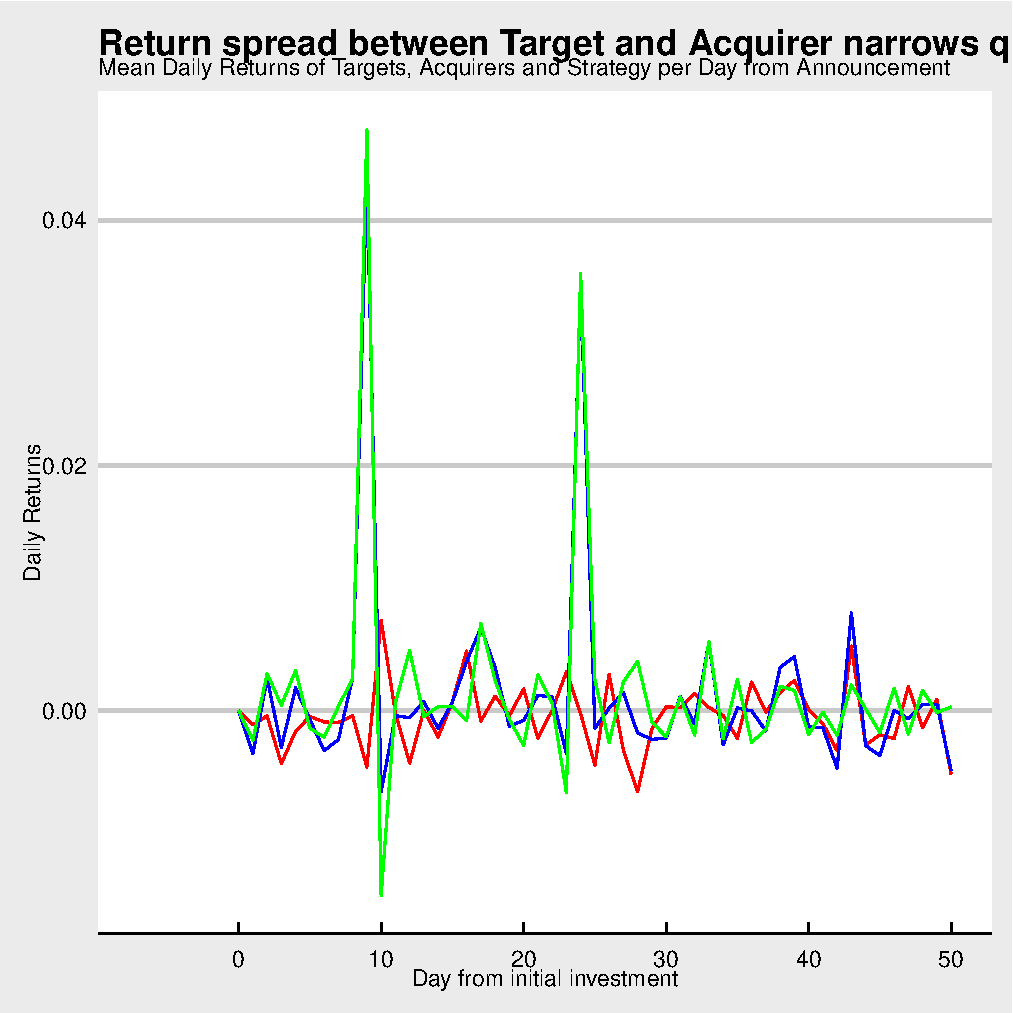
\includegraphics{DataAnalysisvF_files/figure-latex/unnamed-chunk-19-1} \end{center}

Cumulative Return

\begin{Shaded}
\begin{Highlighting}[]
\CommentTok{\# Cumulative return for acquirer}
\NormalTok{initial\_acq\_v2 \textless{}{-}}\StringTok{ }\NormalTok{acq\_tar\_v2 }\OperatorTok{\%\textgreater{}\%}
\StringTok{  }\KeywordTok{filter}\NormalTok{(period }\OperatorTok{==}\StringTok{ }\DecValTok{0}\NormalTok{) }\OperatorTok{\%\textgreater{}\%}
\StringTok{  }\KeywordTok{rename}\NormalTok{(}\DataTypeTok{initial\_acq =}\NormalTok{ close\_acquirer) }\OperatorTok{\%\textgreater{}\%}
\StringTok{  }\KeywordTok{select}\NormalTok{(acquirer, target, initial\_acq) }\OperatorTok{\%\textgreater{}\%}
\StringTok{  }\KeywordTok{distinct}\NormalTok{()}

\NormalTok{cum\_acq\_v2 \textless{}{-}}\StringTok{ }\KeywordTok{left\_join}\NormalTok{(acq\_tar\_v2, initial\_acq\_v2, }\DataTypeTok{by =} \KeywordTok{c}\NormalTok{(}\StringTok{"acquirer"}\NormalTok{, }\StringTok{"target"}\NormalTok{)) }\OperatorTok{\%\textgreater{}\%}
\StringTok{  }\KeywordTok{mutate}\NormalTok{(}\DataTypeTok{cum\_ret\_acq =} \KeywordTok{ifelse}\NormalTok{(period }\OperatorTok{\textgreater{}}\StringTok{ }\DecValTok{0}\NormalTok{, close\_acquirer}\OperatorTok{/}\NormalTok{initial\_acq }\OperatorTok{{-}}\StringTok{ }\DecValTok{1}\NormalTok{, }\OtherTok{NA}\NormalTok{)) }\OperatorTok{\%\textgreater{}\%}
\StringTok{  }\KeywordTok{group\_by}\NormalTok{(period) }\OperatorTok{\%\textgreater{}\%}
\StringTok{  }\KeywordTok{summarise}\NormalTok{(}\DataTypeTok{mean\_cum\_ret\_acq =} \KeywordTok{mean}\NormalTok{(cum\_ret\_acq, }\DataTypeTok{na.rm =}\OtherTok{TRUE}\NormalTok{)) }\OperatorTok{\%\textgreater{}\%}
\StringTok{  }\KeywordTok{filter}\NormalTok{(period }\OperatorTok{\textless{}=}\StringTok{ }\DecValTok{50}\NormalTok{)}
\end{Highlighting}
\end{Shaded}

\begin{Shaded}
\begin{Highlighting}[]
\CommentTok{\# Cumulative return for target}
\NormalTok{initial\_tar\_v2 \textless{}{-}}\StringTok{ }\NormalTok{acq\_tar\_v2 }\OperatorTok{\%\textgreater{}\%}
\StringTok{  }\KeywordTok{filter}\NormalTok{(period }\OperatorTok{==}\StringTok{ }\DecValTok{0}\NormalTok{) }\OperatorTok{\%\textgreater{}\%}
\StringTok{  }\KeywordTok{rename}\NormalTok{(}\DataTypeTok{initial\_tar =}\NormalTok{ close\_target) }\OperatorTok{\%\textgreater{}\%}
\StringTok{  }\KeywordTok{select}\NormalTok{(acquirer, target, initial\_tar)}

\NormalTok{cum\_tar\_v2 \textless{}{-}}\StringTok{ }\KeywordTok{left\_join}\NormalTok{(acq\_tar\_v2, initial\_tar\_v2, }\DataTypeTok{by =} \KeywordTok{c}\NormalTok{(}\StringTok{"acquirer"}\NormalTok{, }\StringTok{"target"}\NormalTok{)) }\OperatorTok{\%\textgreater{}\%}
\StringTok{  }\KeywordTok{mutate}\NormalTok{(}\DataTypeTok{cum\_ret\_tar =} \KeywordTok{ifelse}\NormalTok{(period }\OperatorTok{\textgreater{}}\StringTok{ }\DecValTok{0}\NormalTok{, close\_target}\OperatorTok{/}\NormalTok{initial\_tar }\OperatorTok{{-}}\StringTok{ }\DecValTok{1}\NormalTok{, }\OtherTok{NA}\NormalTok{)) }\OperatorTok{\%\textgreater{}\%}
\StringTok{  }\KeywordTok{group\_by}\NormalTok{(period) }\OperatorTok{\%\textgreater{}\%}
\StringTok{  }\KeywordTok{summarise}\NormalTok{(}\DataTypeTok{mean\_cum\_ret\_tar =} \KeywordTok{mean}\NormalTok{(cum\_ret\_tar, }\DataTypeTok{na.rm =}\OtherTok{TRUE}\NormalTok{)) }\OperatorTok{\%\textgreater{}\%}
\StringTok{  }\KeywordTok{filter}\NormalTok{(period }\OperatorTok{\textless{}=}\StringTok{ }\DecValTok{50}\NormalTok{)}
\end{Highlighting}
\end{Shaded}

\begin{Shaded}
\begin{Highlighting}[]
\CommentTok{\# Combine all}
\NormalTok{cum\_all\_v2 \textless{}{-}}\StringTok{ }\KeywordTok{left\_join}\NormalTok{(cum\_acq\_v2, cum\_tar\_v2, }\DataTypeTok{by =} \StringTok{"period"}\NormalTok{)}
  

\KeywordTok{ggplot}\NormalTok{(cum\_all\_v2) }\OperatorTok{+}
\StringTok{  }
\StringTok{  }\KeywordTok{geom\_line}\NormalTok{(}\KeywordTok{aes}\NormalTok{(}\DataTypeTok{x =}\NormalTok{ period, }\DataTypeTok{y =}\NormalTok{ mean\_cum\_ret\_tar), }\DataTypeTok{colour =} \StringTok{"blue"}\NormalTok{) }\OperatorTok{+}
\StringTok{  }\KeywordTok{geom\_line}\NormalTok{(}\KeywordTok{aes}\NormalTok{(}\DataTypeTok{x =}\NormalTok{ period, }\DataTypeTok{y =}\NormalTok{ mean\_cum\_ret\_acq), }\DataTypeTok{colour =} \StringTok{"red"}\NormalTok{) }\OperatorTok{+}
\StringTok{  }\KeywordTok{theme\_bw}\NormalTok{() }\OperatorTok{+}
\StringTok{  }\KeywordTok{labs}\NormalTok{(}\DataTypeTok{title =} \StringTok{"Mean Cumulative Return"}\NormalTok{,}
       \DataTypeTok{subtitle =} \StringTok{"Investments start 1 day after announcement of potential M\&A deal"}\NormalTok{,}
       \DataTypeTok{y =} \StringTok{"Cumulative Return"}\NormalTok{,}
       \DataTypeTok{x =} \StringTok{"Day from initial investment"}\NormalTok{)}
\end{Highlighting}
\end{Shaded}

\begin{center}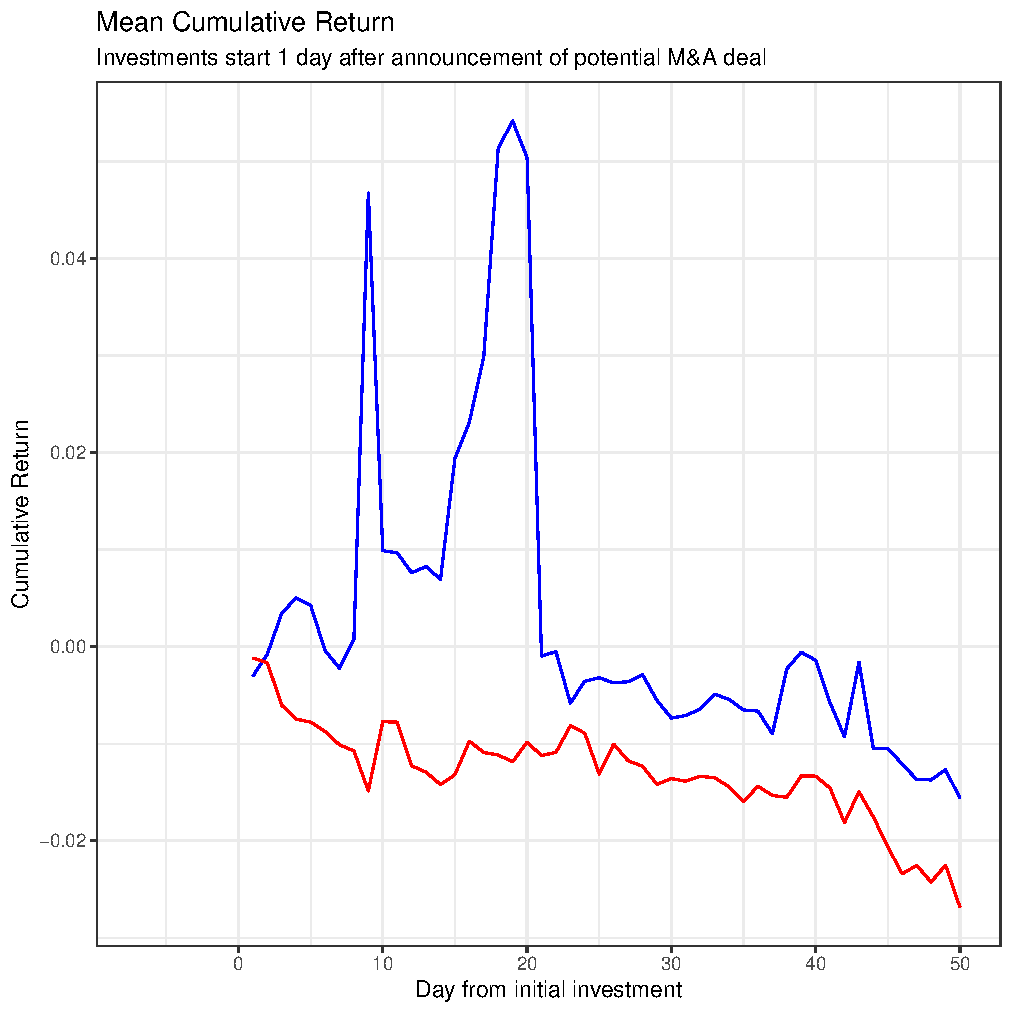
\includegraphics{DataAnalysisvF_files/figure-latex/unnamed-chunk-22-1} \end{center}

Correlation between return and deal completion

Correlation between acquirer return and deal completion

\begin{Shaded}
\begin{Highlighting}[]
\NormalTok{end\_acq\_v2 \textless{}{-}}\StringTok{ }\NormalTok{acq\_tar\_v2 }\OperatorTok{\%\textgreater{}\%}
\StringTok{  }\KeywordTok{mutate}\NormalTok{(}\DataTypeTok{diff =}\NormalTok{ close\_date }\OperatorTok{{-}}\StringTok{ }\NormalTok{date) }\OperatorTok{\%\textgreater{}\%}
\StringTok{  }\KeywordTok{filter}\NormalTok{(diff }\OperatorTok{==}\StringTok{ }\DecValTok{0}\NormalTok{) }\OperatorTok{\%\textgreater{}\%}
\StringTok{  }\KeywordTok{rename}\NormalTok{(}\DataTypeTok{end\_acq =}\NormalTok{ close\_acquirer) }\OperatorTok{\%\textgreater{}\%}
\StringTok{  }\KeywordTok{select}\NormalTok{(acquirer, period, target, end\_acq, DealStatus) }\OperatorTok{\%\textgreater{}\%}
\StringTok{  }\KeywordTok{distinct}\NormalTok{()}


\NormalTok{deal\_ret\_acq\_v2 \textless{}{-}}\StringTok{ }\KeywordTok{left\_join}\NormalTok{(end\_acq, initial\_acq, }\DataTypeTok{by =} \KeywordTok{c}\NormalTok{(}\StringTok{"acquirer"}\NormalTok{, }\StringTok{"target"}\NormalTok{)) }\OperatorTok{\%\textgreater{}\%}
\StringTok{  }\KeywordTok{filter}\NormalTok{(acquirer }\OperatorTok{!=}\StringTok{ "RTX"}\NormalTok{) }\OperatorTok{\%\textgreater{}\%}
\StringTok{  }\KeywordTok{mutate}\NormalTok{(}\DataTypeTok{annualised\_ret =}\NormalTok{ (end\_acq}\OperatorTok{/}\NormalTok{initial\_acq)}\OperatorTok{\^{}}\NormalTok{(}\DecValTok{252}\OperatorTok{/}\NormalTok{period) }\OperatorTok{{-}}\StringTok{ }\DecValTok{1}\NormalTok{) }\OperatorTok{\%\textgreater{}\%}
\StringTok{  }\KeywordTok{group\_by}\NormalTok{(DealStatus) }\OperatorTok{\%\textgreater{}\%}
\StringTok{  }\KeywordTok{summarise}\NormalTok{(}\DataTypeTok{mean\_annualised\_acq\_ret =} \KeywordTok{mean}\NormalTok{(annualised\_ret, }\DataTypeTok{na.rm =} \OtherTok{TRUE}\NormalTok{))}

\NormalTok{deal\_ret\_acq\_v2}
\end{Highlighting}
\end{Shaded}

 
  \providecommand{\huxb}[2]{\arrayrulecolor[RGB]{#1}\global\arrayrulewidth=#2pt}
  \providecommand{\huxvb}[2]{\color[RGB]{#1}\vrule width #2pt}
  \providecommand{\huxtpad}[1]{\rule{0pt}{#1}}
  \providecommand{\huxbpad}[1]{\rule[-#1]{0pt}{#1}}

\begin{table}[ht]
\begin{centerbox}
\begin{threeparttable}
 \label{tab:unnamed-chunk-23}
\setlength{\tabcolsep}{0pt}
\begin{tabular}{l l}


\hhline{>{\huxb{0, 0, 0}{0.4}}->{\huxb{0, 0, 0}{0.4}}-}
\arrayrulecolor{black}

\multicolumn{1}{!{\huxvb{0, 0, 0}{0.4}}l!{\huxvb{0, 0, 0}{0}}}{\huxtpad{6pt + 1em}\raggedright \hspace{6pt} \textbf{DealStatus} \hspace{6pt}\huxbpad{6pt}} &
\multicolumn{1}{r!{\huxvb{0, 0, 0}{0.4}}}{\huxtpad{6pt + 1em}\raggedleft \hspace{6pt} \textbf{mean\_annualised\_acq\_ret} \hspace{6pt}\huxbpad{6pt}} \tabularnewline[-0.5pt]


\hhline{>{\huxb{0, 0, 0}{0.4}}->{\huxb{0, 0, 0}{0.4}}-}
\arrayrulecolor{black}

\multicolumn{1}{!{\huxvb{0, 0, 0}{0.4}}l!{\huxvb{0, 0, 0}{0}}}{\cellcolor[RGB]{242, 242, 242}\huxtpad{6pt + 1em}\raggedright \hspace{6pt} Completed \hspace{6pt}\huxbpad{6pt}} &
\multicolumn{1}{r!{\huxvb{0, 0, 0}{0.4}}}{\cellcolor[RGB]{242, 242, 242}\huxtpad{6pt + 1em}\raggedleft \hspace{6pt} 0.0782 \hspace{6pt}\huxbpad{6pt}} \tabularnewline[-0.5pt]


\hhline{>{\huxb{0, 0, 0}{0.4}}|>{\huxb{0, 0, 0}{0.4}}|}
\arrayrulecolor{black}

\multicolumn{1}{!{\huxvb{0, 0, 0}{0.4}}l!{\huxvb{0, 0, 0}{0}}}{\huxtpad{6pt + 1em}\raggedright \hspace{6pt} Failed \hspace{6pt}\huxbpad{6pt}} &
\multicolumn{1}{r!{\huxvb{0, 0, 0}{0.4}}}{\huxtpad{6pt + 1em}\raggedleft \hspace{6pt} -0.407~ \hspace{6pt}\huxbpad{6pt}} \tabularnewline[-0.5pt]


\hhline{>{\huxb{0, 0, 0}{0.4}}->{\huxb{0, 0, 0}{0.4}}-}
\arrayrulecolor{black}
\end{tabular}
\end{threeparttable}\par\end{centerbox}

\end{table}
 

Correlation between target return and deal completion

\begin{Shaded}
\begin{Highlighting}[]
\NormalTok{end\_tar\_v2 \textless{}{-}}\StringTok{ }\NormalTok{acq\_tar\_v2 }\OperatorTok{\%\textgreater{}\%}
\StringTok{  }\KeywordTok{mutate}\NormalTok{(}\DataTypeTok{diff =}\NormalTok{ close\_date }\OperatorTok{{-}}\StringTok{ }\NormalTok{date) }\OperatorTok{\%\textgreater{}\%}
\StringTok{  }\KeywordTok{filter}\NormalTok{(diff }\OperatorTok{==}\StringTok{ }\DecValTok{0}\NormalTok{) }\OperatorTok{\%\textgreater{}\%}
\StringTok{  }\KeywordTok{rename}\NormalTok{(}\DataTypeTok{end\_tar =}\NormalTok{ close\_target) }\OperatorTok{\%\textgreater{}\%}
\StringTok{  }\KeywordTok{select}\NormalTok{(acquirer, period, target, end\_tar, DealStatus) }\OperatorTok{\%\textgreater{}\%}
\StringTok{  }\KeywordTok{distinct}\NormalTok{()}


\NormalTok{deal\_ret\_tar\_v2 \textless{}{-}}\StringTok{ }\KeywordTok{left\_join}\NormalTok{(end\_tar\_v2, initial\_tar\_v2, }\DataTypeTok{by =} \KeywordTok{c}\NormalTok{(}\StringTok{"acquirer"}\NormalTok{, }\StringTok{"target"}\NormalTok{)) }\OperatorTok{\%\textgreater{}\%}
\StringTok{  }\KeywordTok{filter}\NormalTok{(acquirer }\OperatorTok{!=}\StringTok{ "RTX"}\NormalTok{) }\OperatorTok{\%\textgreater{}\%}
\StringTok{  }\KeywordTok{mutate}\NormalTok{(}\DataTypeTok{annualised\_ret =}\NormalTok{ (end\_tar}\OperatorTok{/}\NormalTok{initial\_tar)}\OperatorTok{\^{}}\NormalTok{(}\DecValTok{252}\OperatorTok{/}\NormalTok{period) }\OperatorTok{{-}}\StringTok{ }\DecValTok{1}\NormalTok{) }\OperatorTok{\%\textgreater{}\%}
\StringTok{  }\KeywordTok{group\_by}\NormalTok{(DealStatus) }\OperatorTok{\%\textgreater{}\%}
\StringTok{  }\KeywordTok{summarise}\NormalTok{(}\DataTypeTok{mean\_annualised\_tar\_ret =} \KeywordTok{mean}\NormalTok{(annualised\_ret, }\DataTypeTok{na.rm =} \OtherTok{TRUE}\NormalTok{))}

\NormalTok{deal\_ret\_tar}
\end{Highlighting}
\end{Shaded}

 
  \providecommand{\huxb}[2]{\arrayrulecolor[RGB]{#1}\global\arrayrulewidth=#2pt}
  \providecommand{\huxvb}[2]{\color[RGB]{#1}\vrule width #2pt}
  \providecommand{\huxtpad}[1]{\rule{0pt}{#1}}
  \providecommand{\huxbpad}[1]{\rule[-#1]{0pt}{#1}}

\begin{table}[ht]
\begin{centerbox}
\begin{threeparttable}
 \label{tab:unnamed-chunk-24}
\setlength{\tabcolsep}{0pt}
\begin{tabular}{l l}


\hhline{>{\huxb{0, 0, 0}{0.4}}->{\huxb{0, 0, 0}{0.4}}-}
\arrayrulecolor{black}

\multicolumn{1}{!{\huxvb{0, 0, 0}{0.4}}l!{\huxvb{0, 0, 0}{0}}}{\huxtpad{6pt + 1em}\raggedright \hspace{6pt} \textbf{DealStatus} \hspace{6pt}\huxbpad{6pt}} &
\multicolumn{1}{l!{\huxvb{0, 0, 0}{0.4}}}{\huxtpad{6pt + 1em}\raggedright \hspace{6pt} \textbf{mean\_annualised\_tar\_ret} \hspace{6pt}\huxbpad{6pt}} \tabularnewline[-0.5pt]


\hhline{>{\huxb{0, 0, 0}{0.4}}->{\huxb{0, 0, 0}{0.4}}-}
\arrayrulecolor{black}

\multicolumn{1}{!{\huxvb{0, 0, 0}{0.4}}l!{\huxvb{0, 0, 0}{0}}}{\cellcolor[RGB]{242, 242, 242}\huxtpad{6pt + 1em}\raggedright \hspace{6pt} Completed \hspace{6pt}\huxbpad{6pt}} &
\multicolumn{1}{l!{\huxvb{0, 0, 0}{0.4}}}{\cellcolor[RGB]{242, 242, 242}\huxtpad{6pt + 1em}\raggedright \hspace{6pt} 0.09 \hspace{6pt}\huxbpad{6pt}} \tabularnewline[-0.5pt]


\hhline{>{\huxb{0, 0, 0}{0.4}}|>{\huxb{0, 0, 0}{0.4}}|}
\arrayrulecolor{black}

\multicolumn{1}{!{\huxvb{0, 0, 0}{0.4}}l!{\huxvb{0, 0, 0}{0}}}{\huxtpad{6pt + 1em}\raggedright \hspace{6pt} Failed \hspace{6pt}\huxbpad{6pt}} &
\multicolumn{1}{l!{\huxvb{0, 0, 0}{0.4}}}{\huxtpad{6pt + 1em}\raggedright \hspace{6pt} -0.17 \hspace{6pt}\huxbpad{6pt}} \tabularnewline[-0.5pt]


\hhline{>{\huxb{0, 0, 0}{0.4}}->{\huxb{0, 0, 0}{0.4}}-}
\arrayrulecolor{black}
\end{tabular}
\end{threeparttable}\par\end{centerbox}

\end{table}
 

Returns of strategy over timeline

Using S\&P 500 index if there is no deal

\begin{Shaded}
\begin{Highlighting}[]
\NormalTok{acq\_tar2\_v2 \textless{}{-}}\StringTok{ }\NormalTok{acq\_tar\_v2 }\OperatorTok{\%\textgreater{}\%}
\StringTok{  }\KeywordTok{group\_by}\NormalTok{(date) }\OperatorTok{\%\textgreater{}\%}
\StringTok{  }\KeywordTok{summarise}\NormalTok{(}\DataTypeTok{ret\_strat =} \KeywordTok{mean}\NormalTok{(ret\_combined))}

\NormalTok{SP\_initial\_v2 \textless{}{-}}\StringTok{ }\NormalTok{benchmark }\OperatorTok{\%\textgreater{}\%}
\StringTok{  }\KeywordTok{filter}\NormalTok{(description }\OperatorTok{==}\StringTok{ "SP\_500"}\NormalTok{) }\OperatorTok{\%\textgreater{}\%}
\StringTok{  }\KeywordTok{filter}\NormalTok{(date }\OperatorTok{\textgreater{}=}\StringTok{ "2014{-}05{-}01"}\NormalTok{) }\OperatorTok{\%\textgreater{}\%}
\StringTok{  }\KeywordTok{arrange}\NormalTok{(date) }\OperatorTok{\%\textgreater{}\%}
\StringTok{  }\KeywordTok{head}\NormalTok{(}\DataTypeTok{n =} \DecValTok{1}\NormalTok{) }\OperatorTok{\%\textgreater{}\%}
\StringTok{  }\KeywordTok{rename}\NormalTok{(}\DataTypeTok{initial\_index =}\NormalTok{ close) }\OperatorTok{\%\textgreater{}\%}
\StringTok{  }\KeywordTok{select}\NormalTok{(}\OperatorTok{{-}}\StringTok{ }\NormalTok{date, }\OperatorTok{{-}}\StringTok{ }\NormalTok{index\_return)}

\NormalTok{benchmark }\OperatorTok{\%\textgreater{}\%}
\StringTok{  }\KeywordTok{filter}\NormalTok{(description }\OperatorTok{==}\StringTok{ "SP\_500"}\NormalTok{) }\OperatorTok{\%\textgreater{}\%}
\StringTok{  }\KeywordTok{arrange}\NormalTok{(date) }\OperatorTok{\%\textgreater{}\%}
\StringTok{  }\KeywordTok{left\_join}\NormalTok{(SP\_initial\_v2, }\DataTypeTok{by =} \KeywordTok{c}\NormalTok{(}\StringTok{"description"}\NormalTok{, }\StringTok{"index"}\NormalTok{)) }\OperatorTok{\%\textgreater{}\%}
\StringTok{  }\KeywordTok{left\_join}\NormalTok{(acq\_tar2\_v2, }\DataTypeTok{by =} \StringTok{"date"}\NormalTok{) }\OperatorTok{\%\textgreater{}\%}
\StringTok{  }\KeywordTok{select}\NormalTok{(date, close, initial\_index, ret\_strat) }\OperatorTok{\%\textgreater{}\%}
\StringTok{  }\KeywordTok{mutate}\NormalTok{(}\DataTypeTok{index\_ret =}\NormalTok{ close}\OperatorTok{/}\KeywordTok{lag}\NormalTok{(close) }\OperatorTok{{-}}\StringTok{ }\DecValTok{1}\NormalTok{,}
         \DataTypeTok{cum\_index\_ret =}\NormalTok{ close}\OperatorTok{/}\NormalTok{initial\_index,}
         \DataTypeTok{ret\_strat\_adjusted =} \KeywordTok{ifelse}\NormalTok{(}\KeywordTok{is.na}\NormalTok{(ret\_strat), index\_ret, ret\_strat)) }\OperatorTok{\%\textgreater{}\%}
\StringTok{  }\KeywordTok{filter}\NormalTok{(date }\OperatorTok{\textgreater{}=}\StringTok{ "2014{-}05{-}01"}\NormalTok{) }\OperatorTok{\%\textgreater{}\%}
\StringTok{  }\KeywordTok{mutate}\NormalTok{(}\DataTypeTok{retplus1 =}\NormalTok{ ret\_strat\_adjusted }\OperatorTok{+}\StringTok{ }\DecValTok{1}\NormalTok{,}
    \DataTypeTok{cum\_ret\_strat =} \KeywordTok{cumprod}\NormalTok{(retplus1)) }\OperatorTok{\%\textgreater{}\%}
\StringTok{  }\KeywordTok{ggplot}\NormalTok{() }\OperatorTok{+}
\StringTok{  }\KeywordTok{geom\_line}\NormalTok{(}\KeywordTok{aes}\NormalTok{(}\DataTypeTok{x =}\NormalTok{ date, }\DataTypeTok{y =}\NormalTok{ cum\_index\_ret), }\DataTypeTok{colour =} \StringTok{"red"}\NormalTok{) }\OperatorTok{+}
\StringTok{  }\KeywordTok{geom\_line}\NormalTok{(}\KeywordTok{aes}\NormalTok{(}\DataTypeTok{x =}\NormalTok{ date, }\DataTypeTok{y =}\NormalTok{ cum\_ret\_strat), }\DataTypeTok{colour =} \StringTok{"green"}\NormalTok{) }\CommentTok{\#\#\#?????}\AlertTok{\#\#\#}\CommentTok{ }
\end{Highlighting}
\end{Shaded}

\begin{center}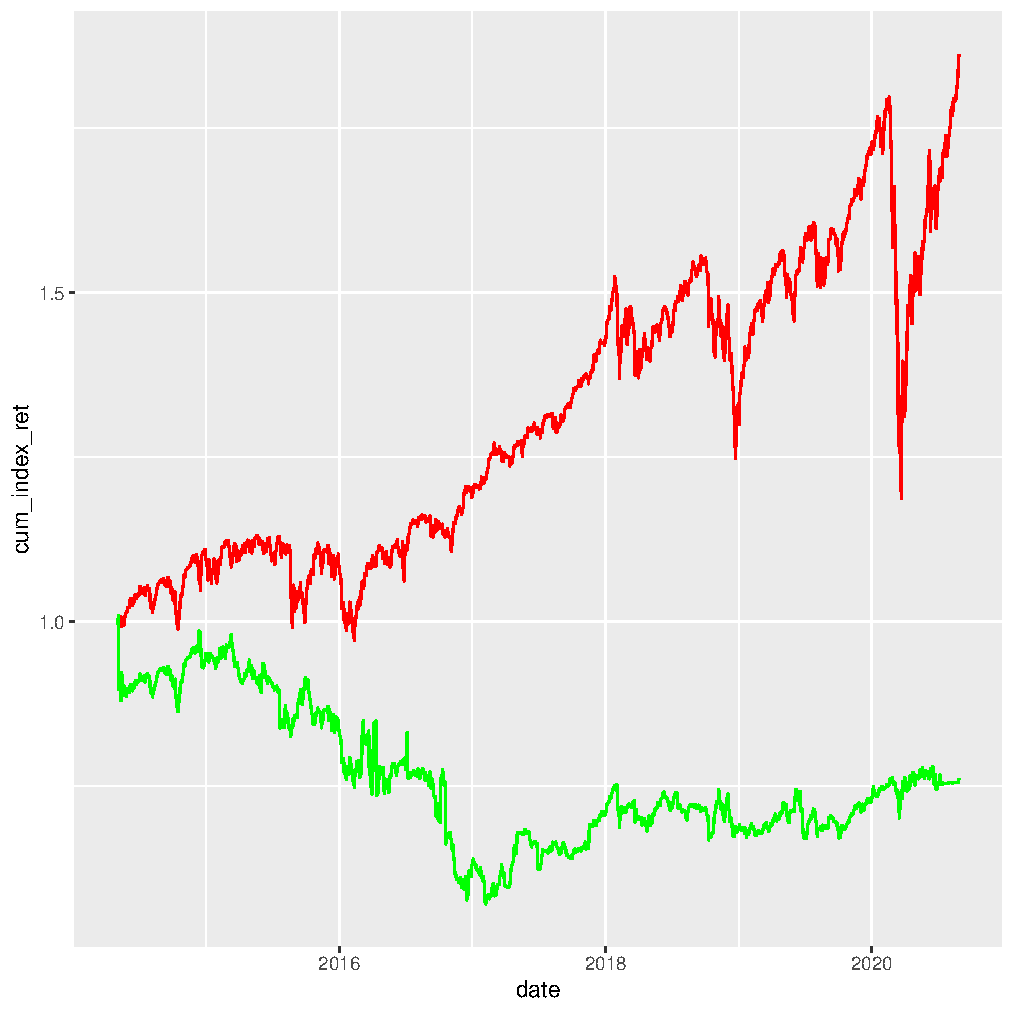
\includegraphics{DataAnalysisvF_files/figure-latex/unnamed-chunk-25-1} \end{center}

Using risk-free rate if there is no deal

\begin{Shaded}
\begin{Highlighting}[]
\NormalTok{benchmark }\OperatorTok{\%\textgreater{}\%}
\StringTok{  }\KeywordTok{filter}\NormalTok{(description }\OperatorTok{==}\StringTok{ "SP\_500"}\NormalTok{) }\OperatorTok{\%\textgreater{}\%}
\StringTok{  }\KeywordTok{arrange}\NormalTok{(date) }\OperatorTok{\%\textgreater{}\%}
\StringTok{  }\KeywordTok{left\_join}\NormalTok{(SP\_initial\_v2, }\DataTypeTok{by =} \KeywordTok{c}\NormalTok{(}\StringTok{"description"}\NormalTok{, }\StringTok{"index"}\NormalTok{)) }\OperatorTok{\%\textgreater{}\%}
\StringTok{  }\KeywordTok{left\_join}\NormalTok{(acq\_tar2\_v2, }\DataTypeTok{by =} \StringTok{"date"}\NormalTok{) }\OperatorTok{\%\textgreater{}\%}
\StringTok{  }\KeywordTok{left\_join}\NormalTok{(tbill, }\DataTypeTok{by =} \StringTok{"date"}\NormalTok{) }\OperatorTok{\%\textgreater{}\%}
\StringTok{  }\KeywordTok{select}\NormalTok{(date, close, initial\_index, ret\_strat, T\_bill\_d) }\OperatorTok{\%\textgreater{}\%}
\StringTok{  }\KeywordTok{mutate}\NormalTok{(}\DataTypeTok{index\_ret =}\NormalTok{ close}\OperatorTok{/}\KeywordTok{lag}\NormalTok{(close) }\OperatorTok{{-}}\StringTok{ }\DecValTok{1}\NormalTok{,}
         \DataTypeTok{cum\_index\_ret =}\NormalTok{ close}\OperatorTok{/}\NormalTok{initial\_index,}
         \DataTypeTok{ret\_strat\_adjusted =} \KeywordTok{ifelse}\NormalTok{(}\KeywordTok{is.na}\NormalTok{(ret\_strat), T\_bill\_d, ret\_strat)) }\OperatorTok{\%\textgreater{}\%}
\StringTok{  }\KeywordTok{filter}\NormalTok{(date }\OperatorTok{\textgreater{}=}\StringTok{ "2014{-}05{-}01"}\NormalTok{) }\OperatorTok{\%\textgreater{}\%}
\StringTok{  }\KeywordTok{mutate}\NormalTok{(}\DataTypeTok{retplus1 =}\NormalTok{ ret\_strat\_adjusted }\OperatorTok{+}\StringTok{ }\DecValTok{1}\NormalTok{,}
    \DataTypeTok{cum\_ret\_strat =} \KeywordTok{cumprod}\NormalTok{(retplus1)) }\OperatorTok{\%\textgreater{}\%}
\StringTok{  }\KeywordTok{ggplot}\NormalTok{() }\OperatorTok{+}
\StringTok{  }\KeywordTok{geom\_line}\NormalTok{(}\KeywordTok{aes}\NormalTok{(}\DataTypeTok{x =}\NormalTok{ date, }\DataTypeTok{y =}\NormalTok{ cum\_index\_ret), }\DataTypeTok{colour =} \StringTok{"red"}\NormalTok{) }\OperatorTok{+}
\StringTok{  }\KeywordTok{geom\_line}\NormalTok{(}\KeywordTok{aes}\NormalTok{(}\DataTypeTok{x =}\NormalTok{ date, }\DataTypeTok{y =}\NormalTok{ cum\_ret\_strat), }\DataTypeTok{colour =} \StringTok{"green"}\NormalTok{) }\CommentTok{\#\#\#?????}\AlertTok{\#\#\#}\CommentTok{ }
\end{Highlighting}
\end{Shaded}

\begin{center}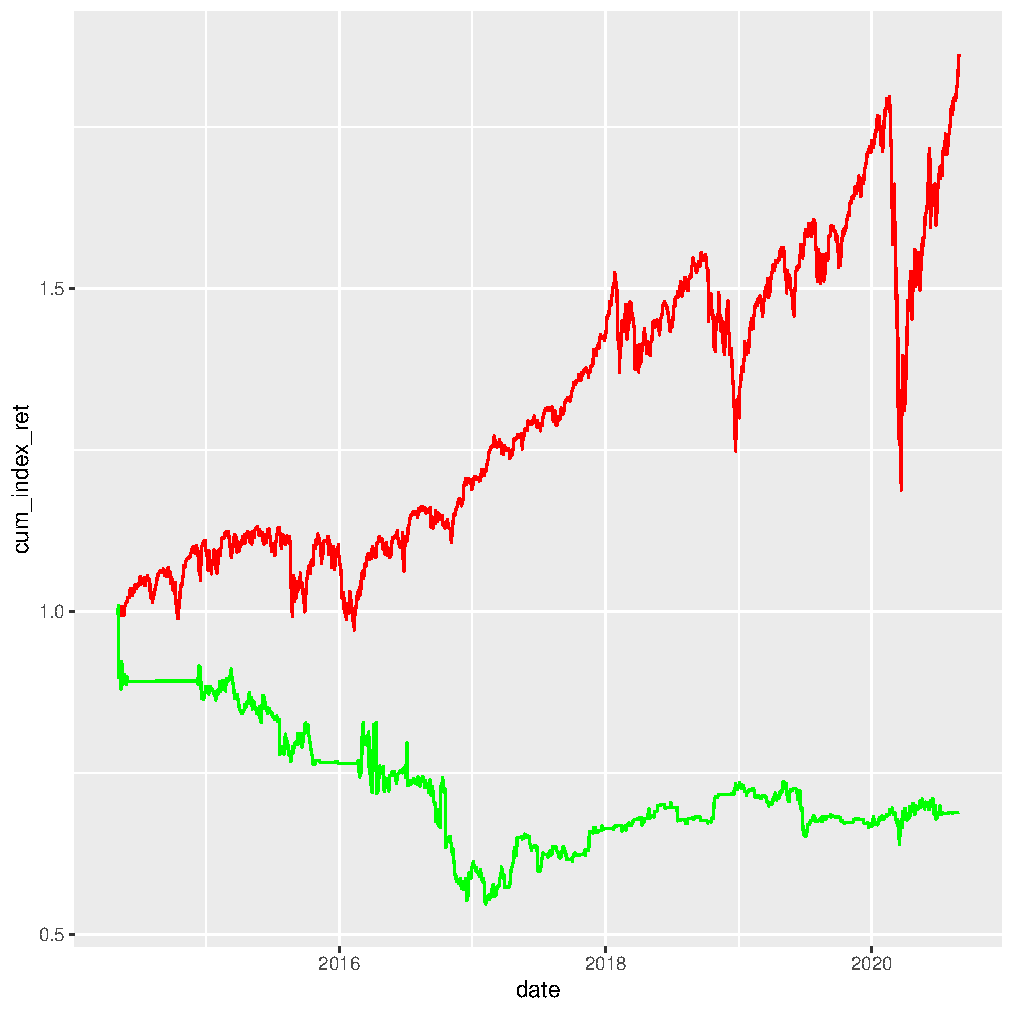
\includegraphics{DataAnalysisvF_files/figure-latex/unnamed-chunk-26-1} \end{center}

CAPM

\begin{Shaded}
\begin{Highlighting}[]
\NormalTok{CAPM\_v2 \textless{}{-}}\StringTok{ }\NormalTok{acq\_tar\_v2 }\OperatorTok{\%\textgreater{}\%}
\StringTok{  }\KeywordTok{left\_join}\NormalTok{(tbill, }\DataTypeTok{by =} \StringTok{"date"}\NormalTok{) }\OperatorTok{\%\textgreater{}\%}
\StringTok{  }\KeywordTok{left\_join}\NormalTok{(benchmarkSP, }\DataTypeTok{by =} \StringTok{"date"}\NormalTok{) }\OperatorTok{\%\textgreater{}\%}
\StringTok{  }\KeywordTok{mutate}\NormalTok{(}\DataTypeTok{Rm\_Rf =}\NormalTok{ SP\_}\DecValTok{500} \OperatorTok{{-}}\StringTok{ }\NormalTok{T\_bill\_d,}
         \DataTypeTok{Rs\_Rf =}\NormalTok{ ret\_combined }\OperatorTok{{-}}\StringTok{ }\NormalTok{T\_bill\_d) }\OperatorTok{\%\textgreater{}\%}
\StringTok{  }\KeywordTok{drop\_na}\NormalTok{(Rm\_Rf, Rs\_Rf) }\OperatorTok{\%\textgreater{}\%}
\StringTok{  }\KeywordTok{filter}\NormalTok{(}\OperatorTok{!}\KeywordTok{is.infinite}\NormalTok{(Rs\_Rf))}

\KeywordTok{ggplot}\NormalTok{(CAPM\_v2, }\KeywordTok{aes}\NormalTok{(}\DataTypeTok{x =}\NormalTok{ Rm\_Rf, }\DataTypeTok{y =}\NormalTok{ Rs\_Rf, }\DataTypeTok{na.rm =} \OtherTok{TRUE}\NormalTok{)) }\OperatorTok{+}
\StringTok{  }\KeywordTok{geom\_point}\NormalTok{() }
\end{Highlighting}
\end{Shaded}

\begin{center}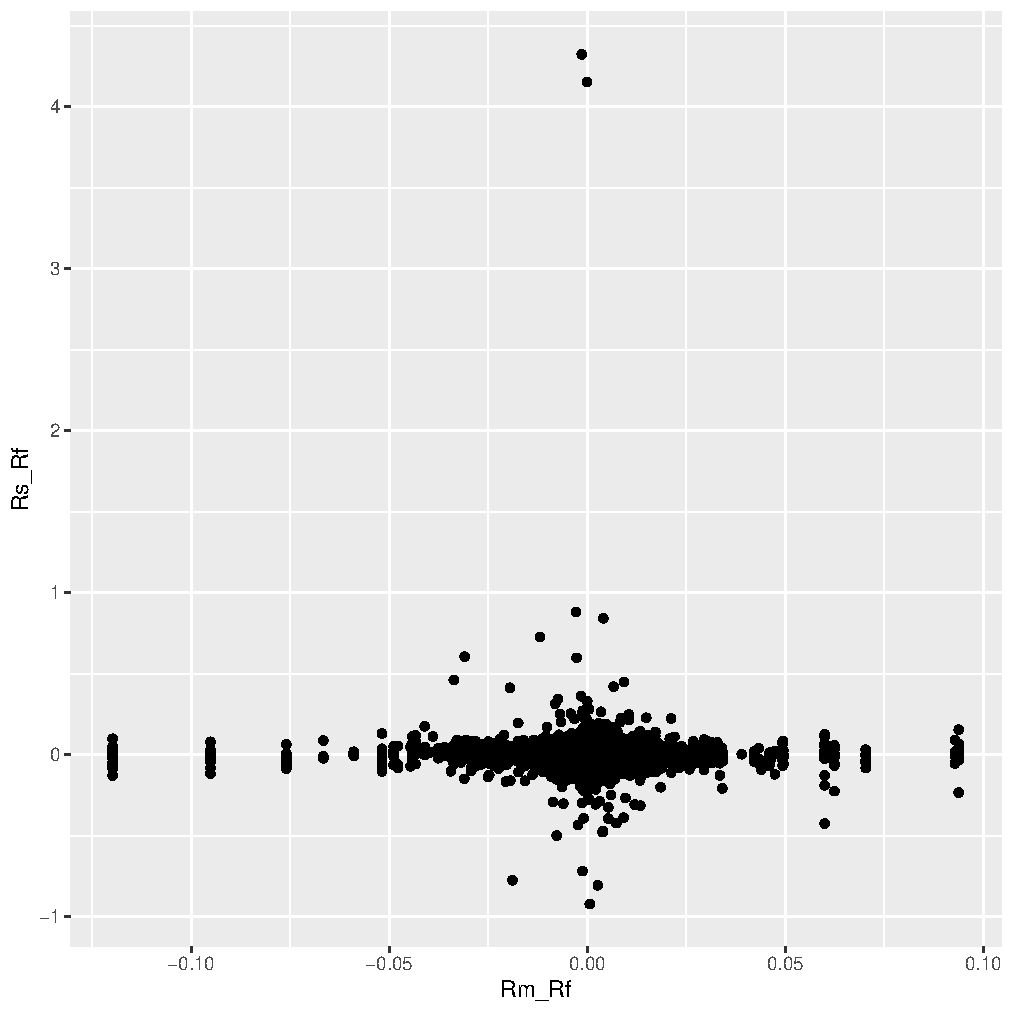
\includegraphics{DataAnalysisvF_files/figure-latex/unnamed-chunk-27-1} \end{center}

\begin{Shaded}
\begin{Highlighting}[]
\NormalTok{CAPM\_regression\_v2 \textless{}{-}}\StringTok{ }\KeywordTok{lm}\NormalTok{(Rs\_Rf }\OperatorTok{\textasciitilde{}}\StringTok{ }\NormalTok{Rm\_Rf, }\DataTypeTok{data =}\NormalTok{ CAPM, }\DataTypeTok{na.rm =}\OtherTok{TRUE}\NormalTok{)}

\NormalTok{CAPM\_regression\_v2}
\end{Highlighting}
\end{Shaded}

\begin{verbatim}
## 
## Call:
## lm(formula = Rs_Rf ~ Rm_Rf, data = CAPM, na.rm = TRUE)
## 
## Coefficients:
## (Intercept)        Rm_Rf  
##    0.005822     0.000526
\end{verbatim}

\begin{Shaded}
\begin{Highlighting}[]
\KeywordTok{huxreg}\NormalTok{(CAPM\_regression\_v2,}
       \DataTypeTok{statistics =} \KeywordTok{c}\NormalTok{(}\StringTok{\textquotesingle{}\#observations\textquotesingle{}}\NormalTok{ =}\StringTok{ \textquotesingle{}nobs\textquotesingle{}}\NormalTok{, }
                      \StringTok{\textquotesingle{}R squared\textquotesingle{}}\NormalTok{ =}\StringTok{ \textquotesingle{}r.squared\textquotesingle{}}\NormalTok{, }
                      \StringTok{\textquotesingle{}Adj. R Squared\textquotesingle{}}\NormalTok{ =}\StringTok{ \textquotesingle{}adj.r.squared\textquotesingle{}}\NormalTok{, }
                      \StringTok{\textquotesingle{}Residual SE\textquotesingle{}}\NormalTok{ =}\StringTok{ \textquotesingle{}sigma\textquotesingle{}}\NormalTok{), }
       \DataTypeTok{bold\_signif =} \FloatTok{0.05}\NormalTok{, }
       \DataTypeTok{stars =} \OtherTok{NULL}
\NormalTok{)}
\end{Highlighting}
\end{Shaded}

 
  \providecommand{\huxb}[2]{\arrayrulecolor[RGB]{#1}\global\arrayrulewidth=#2pt}
  \providecommand{\huxvb}[2]{\color[RGB]{#1}\vrule width #2pt}
  \providecommand{\huxtpad}[1]{\rule{0pt}{#1}}
  \providecommand{\huxbpad}[1]{\rule[-#1]{0pt}{#1}}

\begin{table}[ht]
\begin{centerbox}
\begin{threeparttable}
 \label{tab:unnamed-chunk-27}
\setlength{\tabcolsep}{0pt}
\begin{tabular}{l l}


\hhline{>{\huxb{0, 0, 0}{0.8}}->{\huxb{0, 0, 0}{0.8}}-}
\arrayrulecolor{black}

\multicolumn{1}{!{\huxvb{0, 0, 0}{0}}c!{\huxvb{0, 0, 0}{0}}}{\huxtpad{6pt + 1em}\centering \hspace{6pt}  \hspace{6pt}\huxbpad{6pt}} &
\multicolumn{1}{c!{\huxvb{0, 0, 0}{0}}}{\huxtpad{6pt + 1em}\centering \hspace{6pt} (1) \hspace{6pt}\huxbpad{6pt}} \tabularnewline[-0.5pt]


\hhline{>{\huxb{255, 255, 255}{0.4}}->{\huxb{0, 0, 0}{0.4}}-}
\arrayrulecolor{black}

\multicolumn{1}{!{\huxvb{0, 0, 0}{0}}l!{\huxvb{0, 0, 0}{0}}}{\huxtpad{6pt + 1em}\raggedright \hspace{6pt} (Intercept) \hspace{6pt}\huxbpad{6pt}} &
\multicolumn{1}{r!{\huxvb{0, 0, 0}{0}}}{\huxtpad{6pt + 1em}\raggedleft \hspace{6pt} \textbf{0.006~} \hspace{6pt}\huxbpad{6pt}} \tabularnewline[-0.5pt]


\hhline{}
\arrayrulecolor{black}

\multicolumn{1}{!{\huxvb{0, 0, 0}{0}}l!{\huxvb{0, 0, 0}{0}}}{\huxtpad{6pt + 1em}\raggedright \hspace{6pt}  \hspace{6pt}\huxbpad{6pt}} &
\multicolumn{1}{r!{\huxvb{0, 0, 0}{0}}}{\huxtpad{6pt + 1em}\raggedleft \hspace{6pt} \textbf{(0.003)} \hspace{6pt}\huxbpad{6pt}} \tabularnewline[-0.5pt]


\hhline{}
\arrayrulecolor{black}

\multicolumn{1}{!{\huxvb{0, 0, 0}{0}}l!{\huxvb{0, 0, 0}{0}}}{\huxtpad{6pt + 1em}\raggedright \hspace{6pt} Rm\_Rf \hspace{6pt}\huxbpad{6pt}} &
\multicolumn{1}{r!{\huxvb{0, 0, 0}{0}}}{\huxtpad{6pt + 1em}\raggedleft \hspace{6pt} 0.001~ \hspace{6pt}\huxbpad{6pt}} \tabularnewline[-0.5pt]


\hhline{}
\arrayrulecolor{black}

\multicolumn{1}{!{\huxvb{0, 0, 0}{0}}l!{\huxvb{0, 0, 0}{0}}}{\huxtpad{6pt + 1em}\raggedright \hspace{6pt}  \hspace{6pt}\huxbpad{6pt}} &
\multicolumn{1}{r!{\huxvb{0, 0, 0}{0}}}{\huxtpad{6pt + 1em}\raggedleft \hspace{6pt} (0.311) \hspace{6pt}\huxbpad{6pt}} \tabularnewline[-0.5pt]


\hhline{>{\huxb{255, 255, 255}{0.4}}->{\huxb{0, 0, 0}{0.4}}-}
\arrayrulecolor{black}

\multicolumn{1}{!{\huxvb{0, 0, 0}{0}}l!{\huxvb{0, 0, 0}{0}}}{\huxtpad{6pt + 1em}\raggedright \hspace{6pt} \#observations \hspace{6pt}\huxbpad{6pt}} &
\multicolumn{1}{r!{\huxvb{0, 0, 0}{0}}}{\huxtpad{6pt + 1em}\raggedleft \hspace{6pt} 2213~~~~~ \hspace{6pt}\huxbpad{6pt}} \tabularnewline[-0.5pt]


\hhline{}
\arrayrulecolor{black}

\multicolumn{1}{!{\huxvb{0, 0, 0}{0}}l!{\huxvb{0, 0, 0}{0}}}{\huxtpad{6pt + 1em}\raggedright \hspace{6pt} R squared \hspace{6pt}\huxbpad{6pt}} &
\multicolumn{1}{r!{\huxvb{0, 0, 0}{0}}}{\huxtpad{6pt + 1em}\raggedleft \hspace{6pt} 0.000~ \hspace{6pt}\huxbpad{6pt}} \tabularnewline[-0.5pt]


\hhline{}
\arrayrulecolor{black}

\multicolumn{1}{!{\huxvb{0, 0, 0}{0}}l!{\huxvb{0, 0, 0}{0}}}{\huxtpad{6pt + 1em}\raggedright \hspace{6pt} Adj. R Squared \hspace{6pt}\huxbpad{6pt}} &
\multicolumn{1}{r!{\huxvb{0, 0, 0}{0}}}{\huxtpad{6pt + 1em}\raggedleft \hspace{6pt} -0.000~ \hspace{6pt}\huxbpad{6pt}} \tabularnewline[-0.5pt]


\hhline{}
\arrayrulecolor{black}

\multicolumn{1}{!{\huxvb{0, 0, 0}{0}}l!{\huxvb{0, 0, 0}{0}}}{\huxtpad{6pt + 1em}\raggedright \hspace{6pt} Residual SE \hspace{6pt}\huxbpad{6pt}} &
\multicolumn{1}{r!{\huxvb{0, 0, 0}{0}}}{\huxtpad{6pt + 1em}\raggedleft \hspace{6pt} 0.139~ \hspace{6pt}\huxbpad{6pt}} \tabularnewline[-0.5pt]


\hhline{>{\huxb{0, 0, 0}{0.8}}->{\huxb{0, 0, 0}{0.8}}-}
\arrayrulecolor{black}
\end{tabular}
\end{threeparttable}\par\end{centerbox}

\end{table}
 

\end{document}
